\documentclass[a4paper]{llncs}

%\documentclass{llncs}
%
\usepackage[T1]{fontenc}
\usepackage{lmodern}
\usepackage[utf8]{inputenc}
\usepackage{amsfonts}
\usepackage{eurosym}
\usepackage{amsmath}
\usepackage{amssymb}
\usepackage{booktabs}
\usepackage{makeidx}  % allows for indexgeneration
\usepackage{epsfig} 
\usepackage{cite}
\usepackage{color}
\usepackage{multirow}
\usepackage{mathtools}
\usepackage{subfig}
\usepackage{hyperref}
\usepackage[para]{footmisc}
\hypersetup{
    colorlinks=true,
    %linkcolor=blue,
%    filecolor=magenta,      
    urlcolor=blue,
    citecolor=blue,
    linkcolor=blue,
}

\usepackage[inline]{enumitem}


\usepackage{llncs-space}

\newcommand{\G}{\ensuremath{\mathcal{G}}\xspace}
\newcommand{\X}{\ensuremath{\mathcal{X}}\xspace}
\newcommand{\C}{\ensuremath{\mathcal{C}}\xspace}
\newcommand{\R}{\ensuremath{\mathcal{R}}\xspace}
\newcommand{\PG}{\ensuremath{\mathcal{P}}\xspace}
\newcommand{\PW}{\ensuremath{\mathsf{PW}}\xspace}
\newcommand{\sem}[1]{[|#1|]}
\newcommand{\set}[1]{\{#1\}}
\newcommand{\incl}{\subseteq}
\renewcommand{\L}{\ensuremath{\mathcal{L}}\xspace}

\newtheorem{task}{Task}


%%% \squishlist definition, list with reduced margins
\newcommand{\squishlist}{
 \begin{list}{$\bullet$}
  { \setlength{\itemsep}{0pt}
     \setlength{\parsep}{3pt}
     \setlength{\topsep}{3pt}
     \setlength{\partopsep}{0pt}


     \setlength{\leftmargin}{1em}
     \setlength{\labelwidth}{1em}
     \setlength{\labelsep}{0.5em} } }

\newcommand{\squishlisttwo}{
 \begin{list}{$\bullet$}
  { \setlength{\itemsep}{0pt}
    \setlength{\parsep}{0pt}
    \setlength{	opsep}{0pt}
    \setlength{\partopsep}{0pt}
    \setlength{\leftmargin}{2em}
    \setlength{\labelwidth}{1.5em}
    \setlength{\labelsep}{0.5em} } }

\newcommand{\squishend}{
  \end{list}  }
%\renewcommand{\baselinestretch}{0.99}

\begin{document}
%
\frontmatter          
%



\pagestyle{headings}  

\mainmatter               
%
\title{Qsearch: Answering Quantity Queries from Text}

\author{%
Vinh Thinh Ho$^{1}$,\ \ 
Yusra Ibrahim$^{1}$,\ \ 
Koninika Pal$^{1}$,\\
Klaus Berberich$^{1,2}$,\ \ 
and Gerhard Weikum$^{1}$
}		
\institute{
$^1\ $Max Planck Institute for Informatics, Saarbr\"ucken, Germany\\
$^2\ $Saarland University of Applied Sciences, Saarbr\"ucken, Germany
}


\maketitle        

\begin{abstract}
%%%Motivation and Problem
Quantities appear in search queries in numerous forms: 
%to find a products within a specific price range, 
%to locate a country with an increasing GDP, to identify athletes who won multiple Olympic medals, among others.
companies with annual revenue of at least 50 Mio USD,
athletes who ran 200 meters faster than 19.5 s, 
electric cars with range above 400 miles, and so on.
Processing such queries requires the understanding of numbers present in the query to capture the contextual information about the queried entities. 
Modern search engines and QA systems
%like Google, Bing, etc. 
can 
%efficiently 
handle queries
that involve entities and types, 
%which need to exploit only relational structures embedded in Web content and social media for queried entities. 
%But they fail to produce crisp answers to the queries involving numerical constraints as they disregard the reasoning %over quantitative information.
but they often fail on properly interpreting quantities in queries and candidate answers
when the specifics of the search condition (less than, above, etc.), the units of interest (seconds, miles, meters, etc.)
and the context of the quantity matter (annual or quarterly revenue, etc.).
%  
%Numeric answers for such queries might appear in various sources, either structured (e.g. tables, lists), or unstructured (e.g. text), where processing unstructured text are more challenging. 
%Modern search engines like Google, Bing, etc. support queries that involve relational structures embedded in Web content and social media and can provide crisp answers to the queries or questions. However, informative quantities are usually disregarded. 
%
%Approach and  Contribution
In this paper, we present a search and QA system, called Qsearch, 
that  
%tackles queries with numerical constraints by harnessing quantitative  contextual information about entities from text.
can effectively answer advanced queries with quantity conditions.
%In particular, we propose a framework for representing quantitative information, 
Our solution is based on a deep neural network for extracting quantity-centric tuples from text sources,
%an efficient deep neural network for extracting these information from textual data, 
and a novel matching model to 
%produce 
retrieve and rank
answers 
%for given numerical queries. 
from news articles and other web pages.
Experiments 
%on real-world data 
demonstrate the effectiveness of Qsearch on benchmark queries collected by crowdsourcing.

\end{abstract}

\begin{keywords}
Semantic Search, Question Answering, Information Extraction, 
%Numeric 
Quantities
\end{keywords}

%!TEX root = ../main.tex

\section{Introduction}\label{sec:intro}

\subsubsection{Motivation.}


Quantities, such as \$2B, 40 mpg or 19.19 s,
are more than mere numbers; they express measures 
like revenue, fuel consumption or time in a race
with a numeric value and a corresponding unit. 
The occurrence of a quantity in the text or a table of a web page is associated 
with an entity and interpretable only with the surrounding context. 
%The interpretation of these quantities is only possible through the associated entities and in context. 
For example, in the sentence \textit{``BMW i8 costs about 138k Euros
in Germany and has a battery range between 50 and 60 km.''},
the quantity \euro 138.000 (after normalization) refers to the price
of the car model BMW i8, and the quantity interval [50,60]km
denotes the range for that car (note that this is in electric mode only as this is a hybrid car).

Quantities are common in search queries, for example to find a product within a specific price range,  cars or mobile phones with
desired technical or environmental properties,
or athletes who ran a race in a certain time. 
 When a user issues a quantity search query, such as \textit{``Hybrid cars with price under 35,000 Euros and battery range above 100 km''}, 
 she expects the search engine to understand the quantities and to return relevant answers as a list of entities.
%The relevant answer here is a list of cars that are ``less than 35,000 Euros'' and ``battery range more than 100km''. 
However, Internet search engines treat quantities largely as strings ignoring their values and unit of measurements. As a result, they
cannot handle numeric comparisons, they miss out on units
or scale factors (such as ``k'' in ``138k''), do not know about
necessary conversions between units,  and ultimately
fail. The exceptional cases where search engines 
(incl. vertical product search) provide 
support for coping with quantities are money and date,
but this is achieved by specialized techniques and 
fairly limited. 

\begin{table}[t]
\centering
\captionsetup{justification=centering}
\caption{Statistics on exemplary quantitative properties from Wikidata and DBpedia.\\ %Number of entities with property from Wikidata and DBpedia.\\
\small{\textit{\#E}: number of entities;\ \textit{\#P}: with property present;\ \textit{\#Q}: with explicit data type for the property}.
}
\begin{tabular}{l |r r r|r r r} \midrule
 \multirow{2}{*}{\textbf{~~~~Entity Type/Property}} & \multicolumn{3}{c}{\textbf{Wikidata}} & \multicolumn{3}{|c}{\textbf{DBpedia}}  \\
 \cmidrule{2-7}
 & \textit{~~~~\#E} &  \textit{~~~\#P} & \textit{~~~\#Q~}  & \textit{~~~~\#E} &  \textit{\#P} & \textit{~~~\#Q} \\
 \midrule
%car\_model/top\_speed & 3195 & 3 & 3~ & 6705 & 0 & 0 \\
car model/range & 3195  & 4 & 4~ & 6705 & 0 & 0 \\
car model/engine power & 3195 & 0 & 0~ & 6705 & 0 & 0 \\
mobile phone/display size & 291 & 0 & 0~ & 1358 & 1309 & 0 \\
marathon runner/best time~ & 1629 & 18 & 18~ & 3426 & 1346 & 601 \\
%stadium/capacity & 11233 & 7007 & 7007~ & 11584 & 7818 & 7818 \\
 \midrule
\end{tabular}
\label{table:kg_stats}
\end{table}


One would hope that semantic search over knowledge
graphs (KG) like DBpedia
%, Yago
 or Wikidata goes further,
%but they provide a very low coverage of quantitative facts; 
but their coverage of quantitative facts is very limited
and most literals, apart from dates, are merely represented as strings; e.g., battery capacity of the BMW i3 is shown as the string
\textit{``i3 94 A·h: 33 kWh lithium-ion battery''} in DBpedia.
%display size for mobile phones are represented by number without any associated unit in DBpedia. 
%%The length of the Mercedes-Benz O405 is shown as \textit{``11.1 m''} 
%The weight of the racing car Williams FW07 is shown as \textit{``: 585 kg''} 
%%in DBpedia 
%-- again just a string that is useless for queries with comparisons 
%like vehicles with \textit{``length more than 10 meters''} or \textit{``length above 30 feets''}.
%like cars with \textit{``weight more than 500 kilograms''} or \textit{``weight above 1000 pounds''}.
Important properties for cars, like fuel consumption, CO2 emission, etc. are not covered at all.
%in either DBpedia or Wikidata.
%though these informations are mentioned in additional comments in form of text. 
 Table \ref{table:kg_stats} gives exemplary numbers for the quantity coverage in Wikidata and DBpedia.
%show such low coverage of quantitative facts available in these KGs.
%For some cars like Tesla Model X, the range is shown in the form ``257$\pm$1 mile'' in Wikidata-- again just a string, while API returns simply a point value, 257 mile, rather providing the range that is useless for queries with comparisons 
%the length of the BMW i8 is shown as ``4,689 millimeter'' in Wikidata;
%like ``range above 250 miles''
%or ``range above 400 km''.
% For example, the range of the Tesla Model X is shown as ``257$\pm$1 mile'' in Wikidata -- just a string that is useless for queries with comparisons like ``range above 250 miles'' or ``range above 400 km''; fuel consumption, CO2 emission, etc. are not covered at all.

%Moreover, question answering systems over linked data (incl. KGs)
%have rarely considered quantities in search condition, e.g., a popular benchmark for quantity queries, QALD-6-task-3~\cite{DBLP:journals/semweb/UsbeckRHCHNDU19}, contains only 6 queries with quantity conditions out of 150.

%While range, display size and personal best time are important properties for entity types car, mobile and marathon runner, respectively; these data are not available at all, or the data type is not always included. The exception is stadium capacity, but the number in this case is dimensionless, which is easier to handle.

%Several form-based search engines were created to counter this issue, such as specialized products search engines. However, these form-based search engines are tedious to use and only covers a specific class of items, normally stored in a single relational database. 

%It is complex to find the central entitiy, and 
%uantities appear in search queries in numerous forms: to find a product within a specific price range, to locate a country with an increasing GDP, to explore movies produced in a specific year, to identify athletes who won multiple Olympic medals, among others. They represent an indispensable part of the query that defines the set of the possible answers. Therefore, they necessitate special handling to understand them within their context.

%the current gap in the search engines
 %Natural language queries involving quantities are common. However, modern search engines fail to answer them. Most of the search engines are keyword-based or entity-based.

 %As a result, they treat quantities as a string ignoring their values and unit of measurements.  Moreover, search engines usually retrieve a ranked list of webpages, except for some cases at which search queries involves prominent entities or events.   

%%%GW: now make a crisp statement of what this paper is about
This paper sets out to provide support for answering quantity queries from text, over a wide variety of expressive measures, to overcome
this severe limitation of today's search engines and knowledge graphs.
%GW: added a sentence towards "semantic web"
Our method extracts quantity-centric structure from Web contents, uncovering the hidden semantics
of linking quantities with entities. 

%% what we aim at
%To bridge this gap, we aim at answering quantity queries and providing the user with a seamless search experience.
%We define a quantity query as a query for a specific type of entities, such as cars, that is conditioned on a quantity, such as ``price less than 35,000 Euros''.

%We provide the user with a ranked list of entities, instead of a ranked list of web pages. We pay special attention to quantities in the query and their context while retrieving the answer. Thus, we provide the basis for the next generation search engine capable of answering complex quantity queries. 


 
\subsubsection{Problem Statement.}
We define our problem as follows. Given a quantity query and a corpus of text pages, 
find a ranked list of entities that match the given query.
A quantity query is a triple $(t^*,q^*, X^*)$, where 
$t^*$ is the semantic type of the expected answers, 
$q^*$ is a quantity-centric search condition, and 
$X^*$ is the context that connects the entity type  $t^*$ with quantity condition $q^*$. For example, for the query  \textit{``Cars with price less than \euro 35,000 in Germany''}, the triple $(t^*,q^*, X^*)$ is: $(\textit{cars; < \euro 35.000;} \{\textit{price, Germany}\})$.
%
Our problem has two dimensions.
The first is to understand the content of the text snippets and extract the relevant quantity facts. The second is to match such extracted
assertions (inevitably with noise and errors) against a query
and compute a ranked list of relevant entity answers.


\subsubsection{Approach.}
This paper presents Qsearch, an end-to-end system for answering quantity queries. Qsearch employs a deep neural network
to extract quantity facts from text,
%GW: added a pitch on "semantics"
this way lifting textual information into semantic structures.
%and to understand the users' quantity query. 
Then, it utilizes 
a statistical matching model to retrieve and rank answers.
%On the other hand, we preprocess the corpus of web documents into triples of $(E,Q,X)$, where $E$ is an entity, $Q$ is a quantity related to $E$, and $X$ is the context defining the relation between $E$ and $Q$. For example, the triple \textit{(BMW i8, \{costs, Germany\}, \euro 138.000)} corresponds to the following sentence: \textit{``The BMW i8 costs about \euro 138k in Germany.''}
 %Then, we semantically match the query to the facts we extract from the web corpus. We generate a ranked list of objects matching the query.
%challanges 
%how we do it
%We split the quantity search problem into two essential components: 
%(i)\emph{Quantity-fact extraction from text} (ii)\emph{Query matching}

We model the first component, quantity fact extraction, as a Semantic Role Labeling (SRL) task \cite{DBLP:journals/coling/GildeaJ02} and devise a 
%{Deep Semantic Role Labeling (DSRL)} 
deep learning
method to label words in the sentences with relevant roles. We label each word as entity, quantity or context (or other). Then we use these tags to extract quantity fact triples in form of \textit{(entity, quantity, context)}.
%
For the second component, query matching, we devise a 
%deep 
novel
%semantic
matching method to retrieve a ranked list of relevant entities that answer the user's quantity query.
%more about the approach here!

%We design a full-fledged system that answers complex quantity queries. preprocesses web content, index them, and answers complex quantity queries in an efficient manner.  Our system extracts quantity-related facts from web pages and stores them as a triple of  $(E, Q, X)$. It transforms the problem to a \emph{Semantic Role Labelling} task and employs a \emph{Deep Semantic Role Labeling (DSRL)} model to label sentences. % with $E$, $Q$, and $X$ tags.

%\subsubsection{Limitations of Prior Work.}
%\subsubsection{Outlook}
% research focused on answering quantity queries 
%recent work covering quantity extraction and fact extraction
%QA

%%%GW: this is too long for here (intro)
%Though, some of the previous work tackled, binary and n-ary quantity fact extraction~\cite{DBLP:conf/www/ErnstSW18} and semantic annotation of quantities\cite{DBLP:conf/cikm/IbrahimRW16, Ibrahim:ICDE2019}, none of them looked into how to harness these semantic annotations to answer quantity-related queries. 
%Zhang et al.~\cite{DBLP:conf/sigmod/ZhangC13} consider semantic matching of quantities on web tables, but did not give attention to quantities in natural text.  The work of Banerjee et al.~\cite{DBLP:conf/sigir/BanerjeeCR09} answers quantity consensus queries, however, they only consider binary relations and rely on hand-crafted rules. 
%State of the art retrieval models do not focus on quantity queries nor do they consider extracting quantity facts from the text. On the other hand factoid question answering (QA) systems merely function as a quantity-lookup form structured semantic knowledge. Other QA systems have been proposed to answer reading comprehension questions, however, they do not aggregate answers from multiple sources and they focus on general questions rather than quantity queries. 


%On the other hand, we employ \emph{Deep Semantic Role Labeling  (DSRL)} to extract n-ary quantity facts, and provide a robust system to process and answer quantity queries.

\subsubsection{Contribution.}
The salient contributions of this work are as follows:
\begin{itemize}
\item We present Qsearch, a system for answering quantity queries from text.
\item We propose a deep neural network for quantity fact extraction, and a matching model for answering quantity queries.
\item  We present extensive experiments on benchmark queries collected by crowdsourcing.%, demonstrating the effectiveness of our approach with respect to the correctness of answers.

%\item We make code, data and a running demo available to the research community at\\{\small\url{http://anonymous-for-double-blind-review/}}.
\end{itemize}

\section{Computational Model and System Overview}
In this section, we introduce the computational model for our
approach and give an overview of the Qsearch system and its components.

\subsection{Model for Facts, Queries and Answers}
\label{sec:framework}

%In this paper we present two models, the first is the \texttt{Quantity Fact Extraction} model and the second is the \texttt{Matching} model.
%We formalize the notions of quantity facts, quantity queries
%and answers to queries as follows. 

%In this section, we start by introducing some definitions to lay the foundation for our model. Then, we present our model and specify its inputs and outputs.

%In this section, we introduce our computational model for answering numerical queries, that would be exploited to develop our methodology to extract answers from text later on. In particular, we compose the following definitions:


%This numerical fact representation is quite close to the traditional RDF representation \cite{rdf},  which models each fact as a \textit{(subject, predicate, object)} triple. While the  entity $E$ and quantity $Q$ play as the \textit{subject} and \textit{object} in the RDF model respectively, the context $X$ works like a \textit{predicate}. However, instead of using a unique predicate for all the facts with the same predicate meaning as in the RDF model, we represent $X$ as a set consisting of tokens that could explain the connection between $E$ and $Q$. That is, in a sentence $S$ containing some entity $E$ and quantity $Q$, the context $X$ is determined as a subset of important words from $S$ which could clarify the role of $Q$ with regard to $E$. 


%%%%%%%%%%%%%%%%%%%%%%%%%%%%%%%%% QFE %%%%%%%%%%%%%%%%%%%%%%%
%\subsubsection{Quantity Fact Extraction Model}
\subsubsection{Extraction Model.}
%start from here 
The \textit{input} of this model is a corpus of text documents $\mathcal{T}$ with text snippets (e.g., sentences or paragraphs) that contain
%$n$ 
entity and 
%$m$ 
quantity mentions. 

The \textit{output} of this model is a set of \textit{quantity facts} extracted from the text corpus, $\mathbb{F} =\{\mathcal{F}_1, \mathcal{F}_2, ...\}$, where a quantity fact is defined as follows.


\begin{definition}[Quantity fact] A quantity fact (Qfact) is a triple $\mathcal{F} = (e,q,X)$, where: \\
- $e$ is an entity;\\
- $q = (v,u,r)$ is a quantity consisting of a numerical value $v$, a canonicalized unit $u$ (e.g., km, \$) and a value resolution $r$ (exact, approximate, upper/lower bound, %range
interval);\\
- $X = \{x_1,x_2,...\}$ is a context, which is a bag of words describing the relation between $e$ and $q$.
\end{definition}


\begin{example}
Given the text snippet \textit{``BMW i8 costs about 138k Euros in Germany and has a battery range between 50 and 60 km.''}, we can extract the following Qfacts:\\
- $\mathcal{F}_1: e=\textit{BMW i8}; q=\textit{(138.000, \euro, approximate)}; X = \{\textit{costs, Germany}\}$\\
- $\mathcal{F}_2: e=\textit{BMW i8}; q=\textit{(50-60, km, interval)}; X = \{\textit{range, battery}\}$ 
\qed 
\end{example}


The Qfact representation is similar to the RDF model
\cite{rdf}, 
which
represents each fact as a \textit{(subject, predicate, object)} triple.  In  the Qfact model,  the  entity $e$ and the quantity $q$  correspond to the \textit{subject} and the \textit{object}, respectively. 
The context $X$ in Qfacts is a proxy for the \textit{predicate} in the RDF model. However, it differs in two essential points: first, the context $X$ can capture more than one relation between $e$ and $q$; second, the context $X$ consists of a set of non-canonicalized tokens, instead of a unique canonicalized predicate in a knowledge graph. 

This relaxed representation is a judicious design choice and
essential for the flexibility of our approach: first, we can represent complex n-ary facts using a simple Qfact triple; second, our model can generalize to unseen relations; third, our model can cope with the 
inevitable diversity
and uncertainty in the language expressions of the underlying
text snippets. 
In theory, it is conceivable that all arguments that appear in
the context $X$ are also individually extracted and canonicalized
 to fill the slots of a frame-like structured record.
However, approaches along these lines do not work robustly and
suffer from heavy propagation of noise and errors.


The Qfact model allows different representations of the same fact,
and the underlying text corpus may express the same 
knowledge by different paraphrases. Hence, 
Qfacts are more expressive towards answering queries
via approximate matches and related phrases.
%provides a flexible model to represent the various information expressed in the text.

%%%%%%%%%%%%%%%%%%%%%%%%%%%%%%%%%%%%%%%%%%%%%%%%%%%%%%

%%%%%%%%%%%%%%%%%%%%%%Matching
\subsubsection{Matching Model.}

The \textit{input} of this model is a set of Qfacts $\mathbb{F} =\{\mathcal{F}_1, \mathcal{F}_2, ...\}$
extracted from the text corpus, and  a \textit{quantity query} $\mathcal{Y}$ defined as:


\begin{definition}[Quantity query] A quantity query (Qquery) is a triple $\mathcal{Y} = (t^*,q^*,X^*)$ where: \\
- $t^*$ is the semantic type of the target answers;\\
- $q^* = (v,u,o)$ is a quantity condition consisting of a numerical value $v$, a canonicalized unit $u$ 
(e.g., km, \$)
, and a comparison operator $o$ (exact, approximate, upper/lower bound, 
%range
interval);\\
- $X^* = \{x_1,x_2,...\}$ is a context condition, 
expressed by a bag of words that describes the 
relation between $t^*$ and $q^*$.
\end{definition}

\begin{example}
\label{ex:qquery}
Given the query \textit{``Cars with price less than 100k Euros in Germany''}, its corresponding Qquery is  as follows:\\
- $\mathcal{Y} : t^* = \textit{car}; q^*=\textit{(100.000, \euro, upper bound)}; X^* = \{\textit{price, Germany}\}  $
\qed 
\end{example}

%The definition of the Qquery is analogous to that of the Qfact. Such that, 
Each part of a Qquery imposes a constraint on its 
counterpart in a Qfact considered as a candidate answer.

\begin{definition}[Query answer] 
 A Qfact $ \mathcal{F} =(e,q,X)$ is an answer for a Qquery $\mathcal{Y} = (t^*,q^*,X^*)$ iff 
(1) $e$ is an entity of type $t^*$, 
(2) the quantity $q$ satisfies the quantity condition $q^*$ and (3) the context $X$ (approximately) matches the context condition $X^*$.
\end{definition}

\begin{example}
Consider the Qquery in Example \ref{ex:qquery} and the two text segments
 \textit{``German dealers sell the BMW X3
 at a price as low as 55,000 Euros''} and
 \textit{``Car dealers in Munich sell the BMW X3
starting at 55,000 Euros''}.
The Qfact extracted from the first snippet
with 
$e=\textit{BMW X3},
q=\textit{(55.000, \euro, lower bound)}$,
and $X = \{\textit{German, dealers, sell, price}\}$
is a strong match for the query;
whereas the Qfact extracted from the second snippet
with 
$e = \textit{BMW X3},
q=\textit{(55.000, \euro, lower bound)}$,
and $X = \{\textit{car, dealers, Munich, sell}\}$
is an approximate match (by embedding-based relatedness).
\qed 
\end{example}

The \textit{output} of this model is a ranked list of entities $\mathcal{E}^* = \{e_1, e_2, e_3,...\}$ from matching Qfacts with the Qquery, which will be discussed in Section \ref{sec:match}.

%%%%%%%%%%%%%%%%%%%%%%%%

\subsection{Qsearch System}
Figure \ref{fig:system} 
%shows the high-level architecture of 
gives an overview of the architecture of 
Qsearch. The arrows in the figure depict information flow between the different system components. 
Qsearch consists of two main stages:
\textit{Extract}
and \textit{Answer}.
 
%In this section, we demonstrate our numerical question answering system from text. In Figure \ref{fig:system}, we present a high-level architecture of our system, where the arrows depict information flow between building blocks. We split the working flow of our system into two main stages: \textit{Extract} and \textit{Answer}.

\begin{figure}[t]
\centering
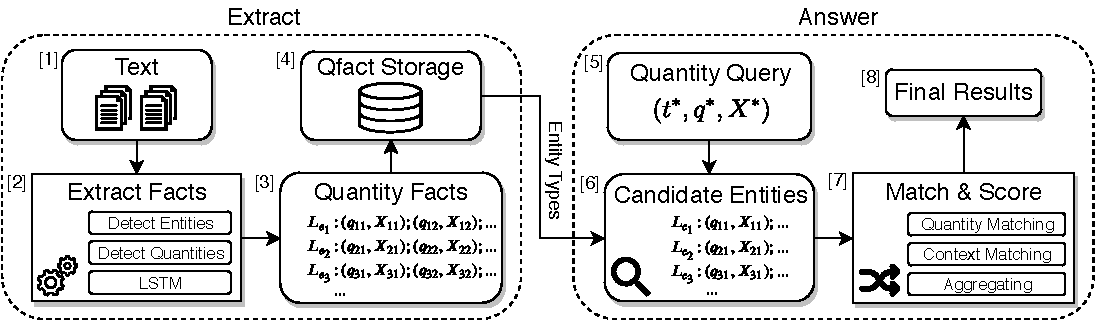
\includegraphics[width=1\textwidth]{figures/overview.pdf}
\caption{Overview of Qsearch.}
\label{fig:system}
\end{figure}
% what is the storage, how is it stored, and indexed 

\subsubsection{Extract.}  
We preprocess the text corpus (Block 1) to recognize
and disambiguate named entities 
%using the AIDA \cite{DBLP:conf/emnlp/HoffartYBFPSTTW11} system,
%which links named entities to the YAGO knowledge base\cite{DBLP:conf/www/SuchanekKW07}. 
and link them to an external knowledge base (KB). We also identify mentions of quantities in the text and normalize them into standard units. 
Subsequently, we run a deep neural network to extract Qfacts from the preprocessed text (Block 2). We learn and employ a specifically designed
Long Short Term Memory (LSTM) network, which will be described in Section \ref{sec:extract}. 

Extracted Qfacts are organized and grouped by their named entities, such that each individual entity $e_i$ is mapped to a list of quantities and related contexts $L_{e_i} = \{(q_{i1},X_{i1}),(q_{i2},X_{i2}),... \}$ (Block 3).
All extracted Qfacts are stored in a data repository (Block 4, 
based on Elasticsearch in our implementation), where entities are linked to their semantic types from the KB.
%We use AIDA \cite{DBLP:conf/emnlp/HoffartYBFPSTTW11} for entity linking, YAGO \cite{DBLP:conf/www/SuchanekKW07} for entity typing, and ElasticSearch as a storage engine.



\subsubsection{Answer.}
We answer incoming Qqueries by matching them against
the Qfacts from the \textit{Extract} stage. 
For a Qquery $(t^*,q^*,X^*)$ (Block 5), we first apply 
an entity-type filter, eliminating entities with the wrong type. 
This results in a set of candidate entities $\mathcal{C} = \{c_1,c_2,...\}$ (Block 6) satisfying the type constraint $t^*$, along with their quantity-context pairs $\{L_{c_1},L_{c_2},...\}$. 
In Block 7, we discard all candidate answers 
%with quantity-context pairs $(q,X) \in L_c$ 
that do not satisfy the quantity condition $q^*$.
Finally, we compute a matching score for each candidate entity $c \in \mathcal{C}$ based on the contexts $X$ in the
quantity-context pairs $L_c$, using a statistical language model
or a text embedding method, which will be described in Section \ref{sec:match}. The candidate entities are ranked by their scores and returned to the user (Block 8). 

In the following Sections
\ref{sec:extract} and \ref{sec:match}, we discuss in detail the
 Qfact extraction model and the matching and answering model, 
respectively.

%In the remainder of this section, we discuss how each candidate entity is scored in Block 7.

\section{Quantity Fact Extraction From Text}
\label{sec:extract}
In this section, we describe our method for extracting Qfacts from natural language text.
%which are then used to answer quantity queries. 
At the core of our solution is a deep-learning neural network for sequence tagging, running on individual sentences. 
%Moreover, we suppose that the input sentence is pre-processed by detecting entities and quantities in advance.

\subsubsection{Input Preprocessing.} In the first step, we preprocess the input text corpus by detecting entities and quantities appearing in each individual input sentence.  
We perform Named Entity Disambiguation (NED) 
using the AIDA \cite{DBLP:conf/emnlp/HoffartYBFPSTTW11} system,
which links named entities to the YAGO knowledge base\cite{DBLP:conf/www/SuchanekKW07}. To achieve a better detection quality, we run NED on a per-document instead of per-sentence basis.
For detecting quantities, we make use of the Illinois Quantifier \cite{DBLP:journals/tacl/RoyVR15}, a state-of-the-art tool for 
recognizing numeric quantities in text, along with some hand-crafted rules (e.g., regular expressions). 
Subsequently, each identified quantity is replaced by a placeholder \textit{``\_QT\_''}. 
\begin{example}
\label{ex:3}
Input and output of this preprocessing step look as follows:
{\small
\begin{align*}
\textit{sentence} &\ |\ \textit{BMW i8 has price of 138k Euros in Germany and range from 50 to 60 km on battery .} \\
\textit{preproce}&\textit{ssed}\ |\ \overbrace{\textit{BMW i8}}^{\mathclap{e_1=\textit{<KB:BMW\_i8>}}}\textit{ has price of }\underbrace{\textit{\_QT\_}}_{\mathclap{q_1=\textit{(138.000,\euro,appr.)}}}\textit{ in }\overbrace{\textit{Germany}}^{\mathclap{e_2=\textit{<KB:Germany>}}}\textit{ and range } \underbrace{\textit{\_QT\_}}_{\mathclap{q_2=\textit{(50-60,km,interval)}}}\textit{ on battery .}  \tag*{\qed}
\end{align*}
%%%GW:  Q - uppercase - is a Qfact. For quantity alone, we should use q - lowercase.
}
\end{example}
\subsubsection{Sequence Tagging Model.} In the second step, we aim to extract complete Qfacts from the preprocessed sentences. 
For each quantity detected in the previous step, we want to identify the entity to which it refers
and the relevant context tokens that express the entity-quantity relation.
\begin{example} 
Consider the preprocessed sentence in Example \ref{ex:3}. If we use the first quantity $q_1 = \textit{(138.000, \euro, approximate)}$
as the input's pivot, 
we want to obtain the output $e(q_1) = e_1 = \textit{<KB:BMW\_i8>}$ and $X(q_1)=\{\textit{price, Germany}\}$. 
Analogously, with $q_2 = \textit{(50-60, km, interval)}$ as pivot,  the desired output is 
$e(q_2)= e_1 = \textit{<KB:BMW\_i8>}$ and $X(q_2)=\{\textit{range, battery}\}$. \qed
\end{example}
We formalize this task as a sequence labeling problem as follows.
\begin{task}[Quantity Fact Extraction]
Given a preprocessed sentence $S$ with the set of detected entities $\mathcal{E} = \{e_1,e_2,...\}$, the set of detected quantities $\mathcal{Q} = \{q_1,q_2,...\}$ and a selected pivot quantity of interest $q_i \in \mathcal{Q}$, the task of quantity fact extraction is to label each token of the sentence with one of the following tags: (i) \textit{<E>}, for denoting the entity that $q_i$ refers to; (ii) \textit{<X>}, for denoting the context tokens that relate $q_i$ and its entity; and (iii) \textit{<O>}, for all other tokens.
\end{task}
\begin{figure}[t]
\centering
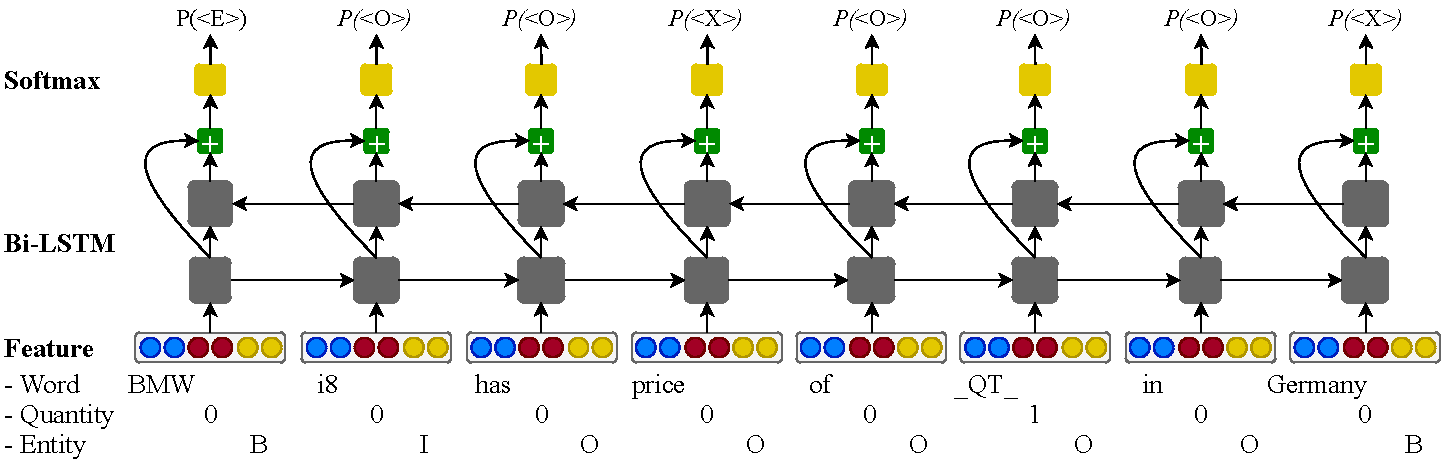
\includegraphics[width=1\textwidth]{figures/neural.pdf}
\caption{The Qfact extraction model used by Qsearch.}
\label{fig:neural}
\end{figure}
Our problem resembles the Semantic Role Labeling task \cite{DBLP:journals/coling/GildeaJ02}, which is typically addressed by
Conditional Random Fields (CRFs)
or Long Short Term Memory (LSTM) models. 
Figure \ref{fig:neural} depicts the bi-directional LSTM model 
that we devised for this task, inspired by prior work \cite{DBLP:conf/acl/HeLLZ17a}.
 Other models for sequence labeling (e.g., \cite{DBLP:conf/acl/ZhouX15, DBLP:conf/emnlp/FitzGeraldTG015})
could be easily incorporated as well. 
Our labeling network consists of three layers: Input Features, Bi-LSTM, and Softmax. 
While this general architecture is close to any other LSTM model, the most unique point here is the input representation,
as described next.

\subsubsection{Input Features.} Each token of the preprocessed input sequence is represented as the concatenation of three input feature vectors:
\begin{enumerate}[label=(\it\roman*)]
\item \textit{Word}: We include word embeddings as an input feature, which enables the neural model to 
generalize to different words having similar meanings.
In our implementation, we use Glove \cite{DBLP:conf/emnlp/PenningtonSM14} precomputed embeddings.
\item \textit{Quantity}: We provide the position of the 
pivot quantity to the model as input. 
When sentences contain multiple quantities (which is a relatively frequent case), our model operates
one quantity at a time and we re-run the model for different quantities.
%which resembles the Semantic Role Labeling task, where the verbs are passed into the input instead of the quantities.
\item \textit{Entity}: We also provide information about the recognized entities as input to the neural model. 
As entities often span multiple tokens, we employ the BIO tagging mechanism \cite{DBLP:conf/acl-vlc/RamshawM95}, where a tag \textit{B} is used for tokens at the beginning of an entity name,
\textit{I} for tokens inside the name, and \textit{O} for other tokens. 
With this representation, the output of the model only needs to tag the first token of a multi-word entity name with \textit{<E>}, 
and subsequent tokens are tagged with \textit{<O>}. Figure \ref{fig:neural} shows an example: \textit{``BMW i8''} is chosen as the entity 
connected with the pivot quantity; only the first token \textit{``BMW''} is tagged as \textit{<E>} in the output.
\end{enumerate}

\subsubsection{Output Constrained Decoding.} The output of the model are the probabilities of each token word in the input belonging to each of the three tags \textit{<E>}, \textit{<X>} and \textit{<O>}, produced by the Softmax layer. 
In neural models, usually the tag with the highest score will be assigned to each token word.
%which results in the highest probability of the whole tag sequence. 
However, this standard technique would not take into account the dependencies between output tags, and hence might give us an invalid tag sequence. To solve this issue, we impose the following two constraints on the output of the model at decoding time, and find the most probable tag sequence satisfying them: \textit{(i)} only one tag \textit{<E>} can appear in the output
(namely, for the one entity to which the pivot quantity refers);
and \textit{(ii)} that tag \textit{<E>} has to be at the start token of an entity name. 


To find the most probable tag sequence, we use Dynamic Programming to decode from left to right. Specifically, we compute subsequences of tags $\textit{Seq}_{i,j,k}$ for every $i \in \{1..n\}$ ($n$ is the sentence length)$; j \in \{\textit{<E>}, \textit{<X>}, \textit{<O>}\};$ and $k \in \{0, 1\}$. Here, $\textit{Seq}_{i,j,k}$ denotes tag subsequence with the highest probability for tokens from position $1$ to position $i$, where the tag of token at position $i$ is $j$, and the subsequence contains $k$ \textit{<E>} tags.
Note that the probability of a tag subsequence is computed as the product of the probabilities of its constituent tags. 
The final tag sequence can be derived at $i = n$.

%The final tag sequence can be derived at position $i = n$.

%We compute subsequence of tags from position 0 to i, denoted as  $\textit{Seq}_{i,j,k}$ where $i \in \{1..n\}; j \in \{\textit{<E>}, \textit{<X>}, \textit{<O>}\};$ and $k \in \{0, 1\}$. Here, $\textit{Seq}_{i,j,k}$ represents that the tag of token at position $i$ is $j$ and $k$ is interpreted as the tag subsequence with the highest probability for tokens from position $1$ to $i$.
%where the tag of token at position $i$ is $j$, and the subsequence contains $k$ \textit{<E>} tags.


\subsubsection{Distant Supervision Training.} As training data is an important factor but difficult to obtain, and manual labeling 
at scale is too 
expensive, we employ distant supervision to generate training data for the Qfact extraction model.
We use unsupervised, pattern-based Open Information Extraction (Open IE) to overlay an n-tuple structure
(with triples or higher-arity tuples) 
on the input text. 
We employ the OpenIE4 tool \cite{DBLP:conf/ijcai/Mausam16} to this end, and then use its output tuples
to generate training data. This process consists of two steps:\\

\noindent \textit{- Step 1: Capture information areas:} We define an \textit{information area} as a subset of tokens from a sentence, which presents complete information about a fact.
We run Open IE on the \textit{unprocessed} sentence to detect all possible tuples expressed by the text. 
Each of these tuples has a confidence score; to ensure the quality of the generated training samples, 
we only keep tuples having a confidence score of at least 0.9. 
Each of the selected tuples corresponds to an information area.
\begin{example} Consider the unprocessed sentence in Example \ref{ex:3}, suppose the following tuples are extracted by Open IE: (1): \textit{(BMW i8; has; price of 138k Euros; in Germany)$^{0.95}$}, (2): \textit{(BMW i8; has; range from 50 to 60 km on battery)$^{0.9}$}, (3): \textit{(BMW i8; has; price of 138k Euros)$^{0.8}$}, (4): \textit{(BMW i8; has; range from 50 to 60 km)$^{0.5}$}, and (5): \textit{(BMW i8; has; price)$^{0.1}$}. We only keep high-confidence tuples (1) and (2), which contain complete information. 
Then the following information areas are chosen for training:
{\small
\begin{align*}
\mathrlap{\underbracket{\phantom{\textit{BMW i8 has }}}_{\textit{(2)}}} \overbracket{\textit{BMW i8 has price of 138k Euros in Germany}}^{\textit{(1)}} and \underbracket{\textit{range from 50 to 60 km on battery}}_{\textit{(2)}} . \tag*{\qed}
\end{align*}
}
\end{example}
\noindent \textit{- Step 2: Transform infomation areas into training samples:} We map the information areas obtained in Step 1 with entities and quantities detected from the preprocessing phase:
{\small
\[
 \mathrlap{\underbracket{\phantom{\textit{<KB:BMW\_i8> has }}}_{\textit{(2)}}} \overbracket{\textit{<KB:BMW\_i8> has price of \_QT\_}_{(1)} \textit{in <KB:Germany>}}^{\textit{(1)}} and \underbracket{\textit{range \_QT\_}_{(2)} \textit{on battery}}_{\textit{(2)}} . \tag*{\qed}
\]
}
With this mapping, information areas yield training samples for the neural network. 
We apply conservative filters so that this self-training process minimizes spurious samples.
First, we keep only information areas that contain exactly one quantity \textit{\_QT\_}, the pivot quantity. 
Second, since English sentences tend to express quantity information in active voice, 
the entity connected to the pivot quantity should appear in the first argument (subject) of the Open IE tuple. 
For instance, information area (1) has two entities \textit{<KB:BMW\_i8>} and \textit{<KB:Germany>};
we choose the former as the one to which quantity \textit{\_QT\_$_{(1)}$} refers. 
Finally, we discard all information areas where the subject of the Open IE tuple contains more than one entity.

At this point, for each information area, we have a quantity and a unique entity to which it refers. 
The context between them is determined from the remaining tokens in the information area based on their Part-of-speech (POS) tags. 
We allow only the following POS patterns to form the context: noun (NN*), verb (VB*), adjective (JJ*), adverb (RB*), and 
foreign  word (FW, to capture out-of-vocabulary names). 
We also use pre-defined stopwords to remove uninformative tokens from the context. 
The resulting Qfact, along with the \textit{<E>,<X>,<O>} tags for its token sequence, becomes a positive training sample.
%Furthermore, to prevent the tagging model from being overly optimistic, we also take into account negative training samples, 
As negative training samples, we collect all information areas where no entity could be identified to relate with the
pivot quantity, i.e., all tokens are tagged as \textit{<O>}.


%{\tt\color{red} GW: need to say more about the actual training - size of training data, which 
%software library, batch size, epoch size, learning rate etc. !!!!!!!!!!}

 
%!TEX root = ../main.tex
\section{Candidate Fact Matching Model} 
\label{sec:match}
This section describes our method to answer Qqueries from the extracted Qfacts. To this end, each Qfact is assigned a score denoting its relevance to the given Qquery.

\subsubsection{Query Parsing.} 
%We implemented a simple parser to transform the user queries into the Qquery format. 
Input questions are mapped into Qqueries by a rule-based parser for recognizing answer type and quantity condition; all other tokens (except stopwords) are included in the query context. The parser uses a dictionary of YAGO types and a dictionary of quantity units. An alternative to this rule-based technique would be to apply the same neural extraction method to questions that we have used to extract Qfacts from text. However, the questions are easier to handle, and the rule-based parser works well. 

\begin{task}[Quantity Fact Scoring] Given Qquery $\mathcal{Y} = (t^*,q^*,X^*)$ and Qfact $\mathcal{F} = (e,q,X)$, compute a distance score $d(\mathcal{F}, \mathcal{Y})$ reflecting the relevance of $\mathcal{F}$ regarding $\mathcal{Y}$.
\end{task}
Without loss of generality, we assume that a lower score denotes a better fact.
%As mentioned in Section \ref{sec:framework}, 
$\mathcal{F}$ should be a high-ranked answer for $\mathcal{Y}$ iff the following three conditions hold:
(1) $e$ is an entity of type $t^*$, 
(2) $q$ satisfies $q^*$, and (3) $X$ is a good (approximate) match for $X^*$.

%\begin{task} [Quantity Fact Retrieval] Given a quantity query $\mathcal{Q}$ and a set of candidate quantity facts $\mathbb{F} = \{\mathcal{F}_1,\mathcal{F}_2,... \}$, return a ranked list of facts $\mathbb{F}_i \subset \mathbb{F}$
%\end{task}
\subsubsection{Entity - Type Matching.} We only consider the Qfact $\mathcal{F}$ if the entity $e$ has type $t^*$. Since the entities from text are linked to an external knowledge base, we make use of the type information from the KB to filter out unsuitable facts for $\mathcal{Y}$. %This is done in Block 6 of the Qsearch overview (Figure \ref{fig:system}).

\subsubsection{Quantity Matching.} We also discard $\mathcal{F}$ if $q$ does not satisfy $q^*$. This is the case when either (1) the units of $q$ and $q^*$ relate to different concepts (e.g. \textit{km} (length) vs. \euro (money)) and are thus incomparable; or (2) their values (after conversion to the same unit) do not match the comparison operator of $q^*$. Since quantity matching is not the focus of our paper, we apply a simple matching method as follows. First, we use hand-crafted rules for unit conversions, re-scaling if needed (e.g., for kilo, mega, etc.), and value normalization. Second, we turn the quantity value into an interval based on its resolution. For example, when the query is about approximate matches, a quantity value $v$ is smoothed into the interval $[v-\delta, v+\delta]$ with a configuration parameter $\delta$. In experiments, we set $\delta$ to 5\% of $v$. A comparison is considered a match when the two intervals overlap, and their units (after conversion and re-scaling) match.

\subsubsection{Context Matching.} If the Qfact $\mathcal{F}$ satisfies the above two constraints, we will consider the similarity between the query context $X^*$ and the fact context $X$. We propose to use the following two approaches for measuring the context relevance: a \textit{probabilistic} and an \textit{embedding-based} approach.\\

\noindent \textbf{Probabilistic Ranking Model.} We adopt the Kullback-Leibler (KL) divergence between the query context $X^*$ and the fact context $X$, which is typically used in statistical language models \cite{DBLP:journals/ftir/Zhai08}. The scoring function is defined as follows:
\begin{align*}
d(\mathcal{F}, \mathcal{Y}) = \textit{KL}(X^*, X) &= H(X^*, X) - H(X^*) \\ &\equiv H(X^*, X) 
= -\sum_{w \in \mathcal{V}} P(w|X^*)\,\log P(w|X)
\end{align*}
where $\mathcal{V}$ is the word vocabulary, $H(X^*)$ is the entropy of $X^*$; $H(X^*, X)$ is the cross entropy between $X^*$ and $X$; and $\equiv$ indicates rank equivalence
(i.e., preserving order). 
Since we are only interested in ranking fact contexts in response to a query context, we can omit $H(X^*)$. The word probability $P(w|X^*)$ for the query context is estimated using Maximum Likelihood Estimation (MLE) on an expanded version $X^*_E$ of $X^*$ as:
\[P(w|X^*) = count(w \in X^*_E)/|X^*_E|\]
To expand a query context, we resort to WordNet \cite{Miller:1995:WLD:219717.219748} and add all synonyms of the context words to it. For the fact context, we estimate the word probability $P(w|X)$ using Jelinek-Mercer smoothing 
%to avoid zero probabilities
 as:
\[P(w|X) = (1 - \lambda) \times count(w \in X)/|X| + \lambda \times P(w|B)\]
This linearly combines the MLE from the fact context $X$ with the MLE obtained from a background corpus $B$. The smoothing parameter $\lambda$ (set to $\lambda=0.1$ in our system) controls the influence of the background corpus on the probability estimate. We construct the background corpus $B$ from all sentences of the entire text corpus that contain at least one quantity (total 39M sentences in our data). \\


%Since these two estimates are very sparse, before calculating, we expand $X^*$ and $X$ using an external resource. Moreover, a smoothing method is applied to avoid zero counts.
%\thinh{Should explain more? which resource, how to expand, which smoothing method.}

\noindent \textbf{Embedding-based Ranking Model}: 
We observed on our data that the query context $X^*$ is often shorter than the fact context $X$, since sentences are often more verbose than the typically short queries. Hence, to measure the distance score of $X$ with regard to $X^*$, we can match tokens between $X^*$ and $X$ using word embedding similarity as follows:
\[d(\mathcal{F}, \mathcal{Y}) = {\bigg(\sum\limits_{u \in X^*} \min\limits_{v \in X}(dist(u,v))\bigg)}/{|X^*|}\]
where $dist(u,v) \geq 0$ is the semantic distance between two words $u$ and $v$ estimated from their pre-computed word embedding vectors \cite{DBLP:conf/emnlp/PenningtonSM14}. 
We use cosine distance in the Qsearch implementation, re-scaled for normalization to [0,1]. 
In the above equation, 
we map each word of query context $X^*$ to its closest word in the fact context $X$ in the embedding space. This scoring formula gives the same weight to every token in the query context $X^*$, which might be misleading, since they could have a different degree of importance.
%Therefore, to increase the impact of more important words and to reduce the role of less %important ones in $X^*$, 
This issue is overcome by giving higher weight to important words and lower weight
to uninformative words, using
%we use 
the following distance function:
\[d(\mathcal{F}, \mathcal{Y}) = \frac{\sum\limits_{u \in X^*} W(u)\min\limits_{v \in X}(dist(u,v))}{\sum\limits_{u \in X^*}W(u)} + 1\]
where $W(u) \geq 0$ is the importance weight of word $u$. 
There are several weighting functions that can be used for $W$ (e.g., \textit{inverse document frequency (idf)}, \textit{term strength}, etc.); we use Robertson’s \textit{idf}\cite{DBLP:journals/jd/Robertson04}. 
We call the above formula the 
\textit{directed embedding distance}, $ded(X^* \rightarrow X)$,
between query and fact contexts.

$ded(X^* \rightarrow X)$ describes how well each word in $X^*$ matches with some other word in $X$, but in many cases it fails to reflect the match between their meaning. The presence of a single word in the fact context $X$ can totally change its meaning. Consider, as a concrete example, the two contexts $X^*=\{\textit{net, worth}\}$ vs. $X = \{\textit{negative, net, worth}\}$. Hence, our idea is to penalize the relevance score with an amount proportional to the directed embedding distance between $X$ and $X^*$.
Specifically, we define the \textit{context embedding distance ($ced$)} that implements this idea:
\begin{align*}
&d(\mathcal{F}, \mathcal{Y}) = ced(X^*, X) = ded(X^* \rightarrow X) \times ded(X \rightarrow X^*)^\alpha \\
=& \Bigg( \frac{\sum\limits_{u \in X^*} W(u)\min\limits_{v \in X}(dist(u,v))}{\sum\limits_{u \in X^*}W(u)} + 1 \Bigg) \times \Bigg( \frac{\sum\limits_{u \in X} W(u)\min\limits_{v \in X^*}(dist(u,v))}{\sum\limits_{u \in X}W(u)} +1 \Bigg)^\alpha 
\end{align*}
Intuitively, our $ced$ measure is the product of two components: (1) $ded(X^* \rightarrow X)$ captures how well query context tokens match with fact context, and (2) $ded(X \rightarrow X^*)$ reflects how much additional terms in $X$ shift its meaning, and hence, should be penalized. Parameter $\alpha \in [0,+\infty)$ controls how much the penalty scaling affects the total score.

\begin{example} Consider the Qquery context $X^* = \{\textit{gross, domestic, product}\}$ and two Qfact contexts $X_1 =$ \{\textit{gross, national, product}\}, $X_2 =$  \{\textit{gross, domestic, product, capita}\}. While we are more inclined to $X_1$ than $X_2$, the directed embedding distance $ded(X^* \rightarrow X_2)$ has a slightly better score than $ded(X^* \rightarrow X_1)$, as it does not penalize the word \textit{``capita''}
(which indicates that the GDP is per capita, not the total GDP). 
In contrast, $ded(X_1 \rightarrow X^*)$ is lower than $ded(X_2 \rightarrow X^*)$ (since \textit{``national''} is close to \textit{``domestic''}), preferring $X_1$ over $X_2$ with regard to $X^*$, which results in the desired ranking based on the context embedding distance $ced$. \qed
\end{example}

\subsubsection{Entity Scoring.} The output of Qsearch is a ranked list of entities from matching Qfacts with the Qquery. 
%In Block 7 of the system overview (Figure \ref{fig:system}), we give 
We assign a score for each candidate entity 
%$c \in \mathcal{C}$ based on its quantity-context pairs $L_{c} = \{(q_{c1},X_{c1}),%(q_{c2},X_{c2}),... \}$. Note that after filtering based on the quantity condition, we only need %to consider context matching.
based on one of the above context distance models and
aggregating over the entity's quantity-context pairs as follows:
\[\textit{score}(c \in \mathcal{C}, \mathcal{Y}) = \min\limits_{(q, X) \in L_c} d(\mathcal{F}=(c,q,X), \mathcal{Y})\]
where $d(\mathcal{F}, \mathcal{Y})$ is either the Kullback-Leibler divergence $\textit{KL}(X^*, X)$ or the context embedding distance
$ced(X^*,X)$.
So when the same candidate entity appears in multiple Qfacts, we pick the best-scoring
Qfact context distance.
%Put differently, we rank candidate entities based on their best fact context, i.e., the one %achieving the lowest distance to the query context.


%!TEX root = ../main.tex

\section{Evaluation}
We run experiments on a Linux machine with 80 CPU cores, 500GB RAM, and 2 GPUs. To evaluate Qsearch, we perform an intrinsic evaluation of our {\em Qfact extraction model} and an extrinsic evaluation of the {\em end-to-end Qsearch system}.
\subsubsection{Dataset.} All experiments use a large collection of news articles, compiled from two real world datasets: the \textit{STICS} project \cite{DBLP:conf/sigir/HoffartMW14} with news from 2014 to 2018, 
and the \textit{New York Times} archive
\cite{nyt}
 %5843811 + 1765538
with news from 1986 to 2008.
In total, our corpus consists of 7.6M documents.
 
\subsection{Intrinsic Evaluation of the Quantity Fact Extraction Model}
%We conduct intrinsic evaluation to examine the quality of our Qfact extraction model of the %\textit{Extract} stage.
\subsubsection{Training setup.}
We implemented the  LSTM network using Theano library,
largely following \cite{DBLP:conf/acl/HeLLZ17a} for the training 
configuration: using Adadelta with $\epsilon = 1e^6$ and $\rho = 0.95$;  \textit{lstm\_hidden\_unit = 300}; \textit{rnn\_dropout\_prob = 0.1}; \textit{batch\_size = 100}.

We extracted training samples from the corpus using the distant-supervision technique as described in Section \ref{sec:extract} and conducted the training process with different settings. 
In the \textit{General} setting, we use all available training data
of 3.2M training samples, where we maintain the ratio 3:1 between the number of positive and negative samples.
We also train our model for three other 
\textit{measure-specific} settings, where only a subset of the training samples is used. In particular, we classify training samples into different categories based on the quantity unit. For example, training samples containing quantities with unit \textit{Kilometer} or \textit{Meter} are chosen to train the model in the \textit{Length} setting, while the ones with unit \textit{US dollar}, \textit{Euro}, etc. are picked for the \textit{Money} setting. 
Among many such categories, we selected the three most prevalent measures \textit{Money}, \textit{Percentage} and \textit{Length}, containing 307K, 235K and 41K training samples, respectively (also with ratio 3:1  between positive and negative samples). 
%to train the corresponding models. 
The trained models are then applied to the entire corpus to extract more Qfacts. 
%Note that the input for the trained models should be compatible with their trained settings.

\subsubsection{Performance of Extraction model.}
As the test data does not have any ground-truth labels, 
we randomly selected 100 samples that contain at least two entities from the output tag sequences, for each training model, and manually assessed their validity.
\begin{table}[t]
\centering
\caption{Evaluation of Qfact extraction model of Qsearch on different settings.}
\begin{tabular}{c |r r r|r r r|r r r|r r r} \midrule
 \multirow{2}{*}{\textbf{Tag}} & \multicolumn{3}{c}{\textbf{Length}} & \multicolumn{3}{|c}{\textbf{Money}}  & \multicolumn{3}{|c}{\textbf{Percentage}}  & \multicolumn{3}{|c}{\textbf{General}} \\
 \cmidrule{2-13}
 & \textit{~Prec.} &  \textit{~~~Rec.} & \textit{~~~~~F1~} & \textit{~Prec.} &  \textit{~~~Rec.} & \textit{~~~~~F1~} & \textit{~Prec.} &  \textit{~~~Rec.} & \textit{~~~~~F1~} & \textit{~Prec.} &  \textit{~~~Rec.} & \textit{~~~~~F1~} \\
 \midrule
\textbf{E} & 0.860 & 0.860 & 0.860 & 0.850 & 0.850 & 0.850 & 0.794 & 0.770 & 0.782 & 0.882 & 0.820 & 0.850 \\
\textbf{X} & 0.650 & 0.849 & 0.736 & 0.717 & 0.844 & 0.776 & 0.659 & 0.827 & 0.734 & 0.728 & 0.713 & 0.721 \\
\textbf{O} & 0.958 & 0.886 & 0.920 & 0.942 & 0.886 & 0.913 & 0.947 & 0.888 & 0.917 & 0.895 & 0.906 & 0.900 \\
 \midrule
\textbf{Macro-avg.} & 0.823 & 0.865 & 0.839 & 0.836 & 0.860 & 0.846 & 0.800 & 0.828 & 0.811 & 0.835 & 0.813 & 0.824 \\
 \midrule
\end{tabular}
\label{table:extract_quality}
\end{table}

We evaluate the quality of the three output labels \textit{<E>}, \textit{<X>} and \textit{<O>} by three measures: \textit{Precision}, \textit{Recall}, and \textit{F1 score}.
The results are shown in Table \ref{table:extract_quality}. 
We observe that all training models perform very well on entity tagging with more than 85\% \textit{F1 score}. 
%This assures that our model can efficiently identify the referred entity for a given quantity. 
%The results also show that the extraction models can capture around 70\% of correct context %tokens of the Qfacts.
We also see that the measure-specific training variants for Length and Money
have slight advantages.

%Moreover, the extraction model also achieves at least 90\% accuracy in identifying \textit{<O>} tag, which helps to reduce the noisy candidates for answer generation step. 

%%%%%%%%%%%%%%%%%%%%%%%%%%%%%%%%%%%%%%%

\subsection{Extrinsic Evaluation of the End-to-End Qsearch System}
We performed the extrinsic evaluation of Qsearch 
on a benchmark of 100  quantity queries, collected by crowdsourcing
and covering four domains: \textit{Finance}, \textit{Transport}, \textit{Sports} and \textit{Technology}. 
These queries capture a wide diversity of measures and units as well as variety in query formulations
(e.g., phrases for the comparison operators); see Table~\ref{table:query_stat}. 
%Conditional phrases are also varies widely, e.g., less than, above, over, etc. 
Anecdotal examples of user queries and their answers produced by Qsearch are shown in Table~\ref{table:example_qa}.
We also considered queries from the QALD-6-task-3 statistical QA benchmark \cite{DBLP:conf/esws/UngerNC16},
but out of total 150 training and test queries, we found only 6 with quantity conditions (as opposed to simpler property lookups).

In this evaluation, we use the Qfact extraction model trained under the \textit{General} setting, as it generalizes to different measures and units.
%Here, we discuss the performance of our system which is built upon the facts extracted from the proposed quantity fact %extraction model trained under the \textit{``General''} setting. 
%!TEX root = ../main.tex

\begin{table}[t]	
	\centering
	\small
	\caption{Statistics of benchmark queries from each domain.}
	\begin{tabular}{l| c c c c l } \midrule
		\multirow{2}{*}{\textbf{Domain}} & \multicolumn{5}{c}{\textbf{Distribution of queries based on unit of quantity}} \\
		\cmidrule{2-6}
		    & \textit{~Money~} & \textit{~Length~} & \textit{~Percentage} & \textit{~Others~}~ & \textit{~Examples for Others}\\ \midrule
		Finance &  76 \% & - & 12 \% & 12 \%~   & ~no. of sales, albums, etc.\\ 
		Transport &   4 \% & 32 \% & -& 64 \%~    &~MPG, mph, horsepower, etc.  \\  
		Sports &   8 \% & 32 \% & -&60 \%~ &  ~sec, years, kg, no. of medals, etc.  \\  
		Technology &  20 \% & 20 \% & 8 \% & 52 \% ~& ~megapixels, Watt, mAh , etc. \\ \midrule 
	\end{tabular}
	\label{table:query_stat}
\end{table} 
%!TEX root = ../main.tex
\begin{table}[t]
	\caption{Anecdotal examples of quantity queries and results from Qsearch.}	
	\small	
	\begin{tabular}{p{.2\textwidth} p{.8\textwidth}} 	 \hline
		Domain & Query \\ \hline
		Finance & \textbf{Q1:} Coal companies with more than 200 Million dollar annual profit\\ 
		Transport & \textbf{Q2:} Sport utility vehicles with engine power at least 150 horsepower \\  
		Sports & \textbf{Q3:} Sprinters who ran 100 meter in less than 10 seconds  \\  
		Technology & \textbf{Q4:} Digital cameras with focal length of lens more than 18 mm\\ \bottomrule 
	\end{tabular}
	\small
	\begin{tabular}{p{.075\textwidth} p{.15\textwidth} p{.775\textwidth}} 
	 \hline
		Query & Result & Corresponding Sentence \\ \hline
		Q1& Duke Energy & Duke Energy had revenue of \$ 23.9 billion and profit of \$ 1.9 billion last year.\\ \hline
		
		Q2 & Ford Escape & Its V-6 engine (the Escape is a four-cylinder) has 270 horsepower, 20 percent more than the Lexus RX330. \\ \hline
		Q3 & Andre Grasse & Andre De Grasse, a 20-year-old from Markham, Ont., has run the 100 metre in under 10 seconds three times this year. \\ \hline
		Q4 & Nikon D7100 & For example, the D7100 can be found in a kit with 18-140 mm and 55-300 mm lenses , so you'll want to use the 55-300 mm and zoom in to 300 mm. \\
		\bottomrule
	\end{tabular}	
	\label{table:example_qa}
\end{table}

\subsubsection{Setup.} 
For each Qquery, we consider top-10 results returned by Qsearch and evaluate 
their relevance and validity by judgements from crowd-workers (using Figure-Eight platform, formerly known as CrowdFlower).
The judges were shown the query, the top-10 entity answers, 
and the corresponding 10 sentences from which the answers were extracted. 
Each result was annotated  as \textit{relevant} or \textit{irrelevant} to the query based on the cue given in its corresponding sentence.
For each query, we collected three judgements and 
used the majority label as gold standard. Overall, we obtained a high inter-annotator agreement with Fleiss' Kappa value of 0.54.

\subsubsection{Baselines.} 
Although our Qsearch system produces entities as main result, we still want to compare it with standard search systems, which produce snippets. 
As there is no other system that can handle quantity queries with crisp entity answers, we use
search systems as baselines that produce text snippets as answers.
Specifically, we ran all benchmark queries on Elasticsearch, locally indexing all sentences of our news corpus,
and on Google web search retrieving the top-10 result snippets.
Elasticsearch uses a text-oriented state-of-the-art ranking model based on BM25.
%

The baselines were given certain advantages, to avoid that Qsearch could be viewed as an unfair competitor.
For Elasticsearch, we consider only sentences that contain an entity and a quantity. For the evaluation, we asked crowd-workers to annotate top-10 results, retrieved from Elasticsearch, as relevant or irrelevant based on whether they spotted a reasonable result for the quantity query.
To evaluate result snippets from Google search, we instructed annotators to be generous, as the result snippets are not well-formed sentences (but could be synthesized from
non-contiguous text segments with ellipses). For example, a text snippet that contains a correct entity and its quantity is considered relevant even if it also contains other entities or quantities. Such instructions to annotators give Google results an advantage because Qsearch results are considered relevant only if both entity and quantity are correctly extracted.
%For both Elasticsearch and Google, we evaluated the top-10 results, sentences or answer snippets, respectively.
%Crowd-workers were asked to annotate these as relevant or irrelevant based on whether they spotted
%a good result for the quantity query. 
%For Google Search, we  collect top-3 result snippets for each query. These snippets are manually annotated as %relevant if they mention a entity and the correct information satisfying the query. 
%For Google, as the result snippets are not well-formed sentences (but could be synthesized fromnon-contiguous text segments with ellipses), the annotators were instructed to be generous.

We also explored several state-of-the-art QA systems over linked open data:
Frankenstein
%\footnote{\url{http://frankenstein.qanary-qa.com/}}
\cite{DBLP:conf/www/SinghRBSLUVKP0V18},
QAnswer
%\footnote{\url{http://qanswer.eu/qa}}
\cite{DBLP:conf/www/DiefenbachMQLSM19},
Platypus
%\footnote{\url{http://askplatyp.us/}}
\cite{DBLP:conf/esws/TanonACS18},
AskNow
%\footnote{\url{https://asknowdemo.sda.tech/}}
\cite{DBLP:conf/esws/DubeyDSHL16}, 
Quint
%\footnote{\url{https://gate.d5.mpi-inf.mpg.de/quint/quint}}
\cite{DBLP:conf/emnlp/AbujabalRYW17},
SPARKLIS
%\footnote{\url{http://www.irisa.fr/LIS/ferre/sparklis/}}
\cite{DBLP:journals/semweb/Ferre17}.
%QAKiS\footnote{\url{http://qakis.org/qakis/index.xhtml}}~\cite{DBLP:conf/semweb/CabrioCAMLG12}.
None of these systems is geared for handling quantity questions, except SPARKLIS, however it can only process quantities without associated unit.
Moreover, their underlying KBs have poor coverage of quantities.
% (c.f., Table \ref{table:kg_stats})
%and thus fail to capture the semantic of quantitative facts. Due to these shortcomings, 
%all of the above mentioned LOD-based QA systems were unable to process our benchmark queries, and therefore we exclude them from further evaluation. 
They failed on almost all of our benchmark queries; so we excluded these systems from our comparative evaluation. 


\subsubsection{Performance of Qsearch. } 
Table \ref{table:performance_qsearch} shows the performance of Qsearch for the four domains and
for all 100 queries together, using the two variants of our ranking models:
KL divergence and context embedding distance ($ced$).
For $ced$ we empirically tune the parameter $\alpha = 3$  based on results from 10
validation queries
disjoint from the 100 test queries. 
We report three metrics: \textit{Precision@k}, \textit{Hit@k} and \textit{Mean-Reciprocal-Rank (MRR)}, 
macro-averaged over queries. 
We do not discuss metrics like Recall or MAP, as these would require exhaustively annotating a huge pool
of candidate answers.

\begin{table}[t]
\caption{End-to-end evaluation of Qsearch.}
\centering
\begin{tabular}{l |cc|cc|cc|cc| cc } \midrule
 \multirow{2}{*}{\textbf{~Metric~~}} & \multicolumn{2}{c}{\textbf{Finance}} & \multicolumn{2}{|c}{\textbf{Transport}} & \multicolumn{2}{|c}{\textbf{Sports}} & \multicolumn{2}{|c}{\textbf{Technology}} & \multicolumn{2}{|c}{\textbf{ All}} \\
 \cmidrule{2-11}
	&  \textit{~KL-div.~}&   \textit{~Emb.~} &  \textit{~KL-div.~} & \textit{~Emb.~} &   \textit{~KL-div.~}&   \textit{~Emb.~} &  \textit{~KL-div.~} & \textit{~Emb.~} &  \textit{~KL-div.~} & \textit{~Emb.~} \\
\midrule
\textbf{Pr.@1} & 0.720 & 0.800 & 0.480 & 0.600 & 0.560 & 0.680 & 0.640 & 0.680 & 0.600 & 0.690  \\
\textbf{Pr.@3} & 0.667 & 0.747 & 0.480 & 0.480 & 0.507 & 0.587 & 0.627 & 0.653 & 0.570 & 0.617 \\
\textbf{Pr.@5} & 0.632 & 0.672 & 0.412 & 0.412 & 0.480 & 0.528 & 0.550 & 0.624 & 0.519 & 0.559  \\ 
\textbf{Pr.@10} & 0.604 & 0.608 & 0.333 & 0.379 & 0.412 & 0.432 & 0.500 & 0.547 & 0.462 & 0.492 \\ 
\midrule
\textbf{Hit@3} & 0.880 & 0.920 & 0.760 & 0.760 & 0.760 & 0.800 & 0.840 & 0.880 & 0.810 & 0.840 \\
\textbf{Hit@5} & 0.880 & 0.960 & 0.760 & 0.760 & 0.920 & 0.840 & 0.840 & 0.920 & 0.850 & 0.870 \\ 
\midrule
\textbf{MRR} & 0.792 & 0.870 & 0.621 & 0.678 & 0.685  & 0.746 & 0.747 & 0.783 & 0.711 & 0.769 \\
 \midrule
\end{tabular}
\label{table:performance_qsearch}
\end{table}

%\textbf{Pr.@1} & 0.240 & 0.720  &  0.800 & 0.240& 0.480  &  0.600 & 0.200 & 0.560 & 0.680 & 0.320 & 0.640  &  0.680  \\
%\textbf{Pr.@3} & 0.307 &  0.667 & 0.747 & 0.213 & 0.480 & 0.480  & 0.213 & 0.507  & 0.587 & 0.347 & 0.627  &  0.653  \\
%\textbf{Pr.@5} & 0.248 & 0.632  & 0.672 & 0.184 & 0.412  &  0.412 & 0.184 & 0.480  & 0.528 & 0.320 & 0.550  &  0.624  \\ 
%\textbf{Pr.@10} & 0.220 & 0.604  & 0.608 & 0.136 & 0.333  & 0.379 & 0.164 & 0.412  & 0.432 & 0.324 & 0.500  &   0.547  \\ 
%\midrule
%\textbf{Hit@3} & 0.520 & 0.880  & 0.920 & 0.520 & 0.760  & 0.760  & 0.440 & 0.760  & 0.800 & 0.560 &  0.840  &  0.880  \\
%\textbf{Hit@5} & 0.680 & 0.880  & 0.960 & 0.560 & 0.760  & 0.760  & 0.600 & 0.920  & 0.840 & 0.640 & 0.840  & 0.920   \\ 
%\midrule
%\textbf{MRR} & 0.408 & 0.792  & 0.870 & 0.379 & 0.621 & 0.678 & 0.357 & 0.685  & 0.746 & 0.468 & 0.747  &  0.783  \\

\begin{figure}[t]
	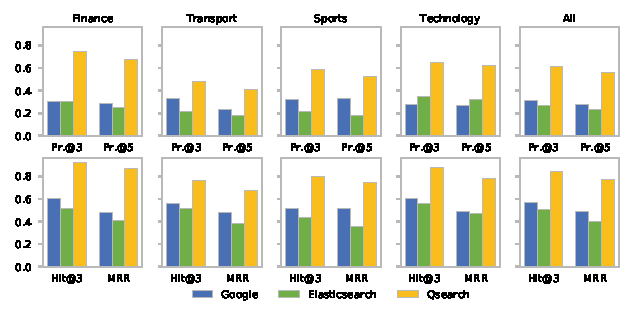
\includegraphics[width= 1\textwidth]{figures/compare.pdf}
	\caption{Comparison of Qsearch against baselines.}
	\label{fig:top-3_comparison}
\end{figure}

Overall, Qsearch performs amazingly well, typically with MRR around 0.7 or better.
The best results are for the 
Finance domain, which has the highest share in the corpus and is most represented in the
Qfact extraction training.
%Finance is the dominating slice of news articles and it covers two most frequent sample categories, Money and %Percentage, in our training dataset. 
%We can also observe that \textit{Precision@k} decreases sharply as \textit{k} increases, together with a high %\textit{MRR} and \textit{Hit} values for our both ranking models, which confirms that relevant entities are ranked higher %by our system than the irrelevant ones. 
\textit{Precision@1} is pretty good, but precision drops substantially when going deeper in the rankings. 
The embedding-based ranking model clearly outperformed the KL-divergence method
by a significant margin.
 
Figure~\ref{fig:top-3_comparison} presents the comparison of Qsearch with the $ced$ ranking model 
against Elasticsearch and Google, showing the metrics \textit{Prec.@3}, \textit{Prec.@5}, \textit{Hit@3} and \textit{MRR}. The results 
clearly indicate that Qsearch outperforms both baselines by a large margin.













%!TEX root = ../main.tex

\section{Related Work}
\label{sec:related-work}

%%%GW: keep this concise
%%% if we discuss QA at length, it suggests that these prior works are highly relevant and we should have compared to them

\subsubsection{Question Answering.} 
%Many advanced factoid-based Question Answering (QA) systems have been developed, covering the both major paradigms in QA, IR-based QA on text corpora \cite{DBLP:conf/acl/WangN15, DBLP:conf/emnlp/YangYM15} and knowledge-based QA\cite{ DBLP:conf/coling/BaoDYZZ16, DBLP:conf/ecctd/Sanchez-Azqueta17}, or fusing them both \cite{DBLP:conf/acl/DasZRM17,DBLP:conf/emnlp/SunDZMSC18}, in order to handle complex compositional queries in natural language. Diverging from traditional open-domain QA, many recently developed QA systems\cite{DBLP:journals/corr/WestonBCM15,DBLP:conf/acl/RajpurkarJL18} address the reading comprehension task that requires understanding and reasoning of natural language.  However, none of these QA systems can efficiently handle processing and reasoning of quantitative information. A few state-of-the-art works\cite{DBLP:conf/cikm/JiaARSW18} focus explicitly the reasoning of temporal constraints in questions, and most of the previous works can support mainly the counting-based numeric queries. In this work, we aim to generalize the processing of quantitative information over varied numerical constraints exploiting deep semantic role labeling. Limited number of numeric relations in the Knowledge is an important bottle neck for processing quantities, and recently has been addressed in\cite{DBLP:conf/aaai/MadaanMMRS16}. Unlike our quantity-specific context extraction model, the authors presented NumberTron which aims to extract triplets for specific numeric relations from textual corpora. Tapping into semi-structured resources from Web, QEWT\cite{DBLP:conf/kdd/SarawagiC14} harnesses ambiguous and imprecise numbers in web tables and improve the performance of quantity-seeking queries.   
%KP: discussion about WikiTableQuestions ?
QA over knowledge graphs and other linked data sources has received great attention over the
last years; see \cite{DBLP:conf/rweb/UngerFC14,DBLP:journals/kais/DiefenbachLSM18} for surveys.
State-of-the-art methods 
(e.g., \cite{DBLP:conf/acl/YihCHG15,DBLP:conf/cikm/BastH15,DBLP:conf/acl/XuRFHZ16,DBLP:conf/www/AbujabalRYW18,DBLP:journals/pvldb/ZhengYZC18}) 
translate questions into
SPARQL queries, bridging the gap between
question vocabulary and the terminology
of the underlying data by means of
templates and/or learning from
training collections of question-answer pairs.
Benchmarks like the long-standing 
QALD series and other competitions
have shown great advances along these lines
\cite{DBLP:journals/semweb/UsbeckRHCHNDU19}.
However, these benchmark tasks hardly
contain any quantity queries of the kind
addressed here (even in QALD-6-task-3, only 6 out of 150 questions are of this kind, others are mostly about quantity lookup). Note that look-ups of 
quantity attributes of qualifying entities
(e.g., Jeff Bezos's net worth, 10 richest people, or fastest sprinter over 100m)
are of a different nature, as they do not
contain quantity comparisons between query
and data (e.g., worth more than 50 million USD,
running faster than 9.9 seconds).
Moreover, the scope and diversity of the benchmark queries is necessarily restricted to relatively
few numeric properties, as knowledge graphs
hardly capture quantities in their full extent (with value and unit properly
separated and normalized). This is our motivation to tap
into text sources with more extensive coverage.

QA over text has considered a wide range
of question types (e.g., \cite{DBLP:conf/emnlp/Yang0ZBCSM18,DBLP:conf/acl/GardnerC18,DBLP:conf/acl/ChenFWB17}), but there
is again hardly any awareness of quantity queries.
Keyword search, including
telegraphic queries, with quantity conditions
have been considered by 
\cite{DBLP:conf/emnlp/JoshiSC14}, and have been applied
to web tables \cite{DBLP:journals/pvldb/PimplikarS12,DBLP:conf/kdd/SarawagiC14}. 
%The approaches pursued in that context
%cannot be carried over to our setting
%where the data input is arbitrary natural language text.

\cite{DBLP:conf/sigir/BanerjeeCR09} and
its follow-up work \cite{DBLP:conf/kdd/SarawagiC14}
focused on
a specific kind of quantity query, namely,
retrieving and aggregating numerical values
associated with an attribute of a given entity
(e.g., Bezos's net worth or GDP of India). To this end, 
learning-to-rank techniques over value distributions
were developed to
counter the uncertainty in the retrieved values,
where web pages often contain crude estimates
and lack exact values.
In contrast to our setting, that work did not
consider quantities in search conditions. 
%and did not
%require inferring units and entities to which
%quantities refer.



\subsubsection{Information Extraction.}
Recognizing and extracting numeric expressions
from text has been addressed using
techniques like CRFs and LSTMs 
(e.g., \cite{DBLP:conf/aaai/MadaanMMRS16,DBLP:conf/acl/SahaPM17,DBLP:conf/sigir/AlonsoS18}).
However, this alone does not turn numbers
into interpretable quantities, with units
and proper reference to the entity with
that quantity. Only few works attempted
to canonicalize quantities by mappings
to hand-crafted knowledge bases 
of measures \cite{DBLP:conf/cikm/IbrahimRW16}, but these efforts are
very limited in scope.
The special case of temporal expressions
has received substantial attention
(e.g., \cite{DBLP:series/synthesis/2016Strotgen}), but this solely covers dates
as measures.

Most related to our approach are the works
of \cite{DBLP:conf/kdd/SarawagiC14} and \cite{DBLP:journals/tacl/RoyVR15}.
The former used probabilistic context-free grammars
to infer units of quantities, but focused specifically
on web tables as inputs.
The latter extended semantic role labeling (see below)
to extract quantities and their units from
natural language sentences.
Neither of these can be readily applied
to extracting quantities and their reference entities
from arbitrary textual inputs.
\subsubsection{Semantic Role Labeling.} Semantic role labeling (SRL) has been intensively researched
as a building block for many 
NLP tasks \cite{DBLP:journals/coling/GildeaJ02}.
%Question Answering frameworks \cite{DBLP:conf/emnlp/ShenL07, DBLP:journals/coling/SurdeanuCZ11}, as well as, in other NLP tasks, such as Information Extraction \cite{DBLP:conf/kcap/ChristensenMSE11, DBLP:conf/naacl/StanovskyMZD18}, Machine translations \cite{DBLP:conf/coling/LiuG10}, in order to exploit the semantic representation of the predicate-argument structure of a sentence in a language. 
Given a verb phrase of a sentence
viewed as a central predicate, 
%the SRL task is to assign different pre-defined roles of the verb in the sentence. 
SRL identifies phrases that are assigned to
pre-defined roles to form a frame-like
predicate-arguments structure.
%Generally, SRL \cite{DBLP:journals/coling/GildeaJ02, DBLP:conf/conll/KoomenPRY05} is considered as a classification task based on syntactic features of sentences and often uses labeled corpus, such as PropBank \cite{DBLP:journals/coling/PalmerKG05}, FrameNet \cite{DBLP:journals/lre/Baker12}. 
%
%Instead of relying on fine-tuned syntactic features of sentences, many recent literature consider word embeddings as one of the key features to learn SRL model using different  neural network methods \cite{DBLP:conf/acl/ZhouX15, DBLP:conf/acl/HeLLZ17a, DBLP:conf/emnlp/FitzGeraldTG015}. 
Modern SRL methods make use of pre-computed
word embeddings and employ deep neural networks
for role filling (e.g., \cite{DBLP:conf/acl/ZhouX15, DBLP:conf/acl/HeLLZ17a, DBLP:conf/emnlp/FitzGeraldTG015}).
%
%Task1 of this work addresses conceptually similar to the SRL task. However, we map a sentence to a general semantic representation based on different quantity-specific roles for a given numeric value from the sentence. Hence, the characteristics of these roles differ from the predicate-argument roles where verbs are technically considered as predicates. In order to learn our quantity-specific SRL model, we employ word-embedding based deep SRL model \cite{DBLP:conf/acl/HeLLZ17a}.
Our approach differs from this state-of-the-art SRL,
as we are not primarily focused on the verb-phrase
predicate, but consider the numeric quantity in a sentence
as the pivot and aim to capture quantity-specific roles.

%%%GW: need to trim the following
To support exploration of quantitative facts in financial reports, \cite{Lamm2018QSRLA} proposed a 
semantic representation for quantity-specific roles.
% and discuss possibilities to utilize the shallow semantic parsing to develop their proposed framework. 
%In the similar direction, in order to solve the elementary school math problems, 
\cite{DBLP:journals/tacl/RoyVR15} devised a quantity representation as an additional component of
an SRL method, which is part of the Illinois Curator software suite.
% to reason about numbers in natural language. 
%
%Our SRL model represents a simplified version of their proposed semantic roles. For example, the roles \textit{entity}, \textit{value}, \textit{unit}, and \textit{resolution} are respectively similar to the roles  \textit{THEME}, \textit{VALUE with SIGN}, \textit{UNIT}, and \textit{MANNER} in their model. However, the  \textit{context} in our model generalizes the roles  \textit{QUANTITY}, \textit{LOCATION}, and \textit{TIME} together from QSRL model by Lamm et al. \cite{Lamm2018QSRLA}. Such generalization of semantic role makes our model simpler and helps in leveraging the problem of numerical Question Answering, addressed in this work. 
Our approach makes use of this technique,
%which is part of the Illinois Curator software suite,
as a preprocessing step.
However, we go further by 
learning how to connect quantities with their
respective entities and to collect relevant 
context cues that enable our matching and
ranking stage for query answering.




%!TEX root = ../main.tex

\section{Conclusion}
%We presented a method for learning rules that may contain negated atoms from KGs that
%dynamically exploits feedback from a precomputed embedding model. 
%Our approach is general in that any embedding model can be utilized including text-enhanced ones, which indirectly allows us to 
%harness
%unstructured 
%web sources 
%for rule learning.
% We evaluated our approach with various configurations on real-world datasets and observed significant improvements
%over state-of-the-art rule learning systems.\looseness=-1
%
%An interesting future direction is to extend our work to more complex non-monotonic rules with higher-arity predicates,
%aggregates and existential variables or disjunctions in rule heads, which is challenging due to inevitable scalability issues.

Awareness of entities and types has greatly advanced semantic search
both for querying the web of linked data and for Internet search engines.
In contrast, coping with quantities in text content and in query constraints
has hardly received any attention, yet is an important case.
This paper has presented the Qsearch system for full-fledged support of
quantity queries, through new ways of information extraction and 
answer matching and ranking.
We capture quantities in their full extent, including units of measures,
reference entities and the relevant contexts.
The model for Qfacts and Qqueries is relatively simple but highly versatile and effective.
%a more detailed structured modeling would not be able to cope with the
%uncertainty in textual inputs and the approximate matching of candidate answers.
A key asset of Qsearch is its high quality in extracting Qfacts,
recognizing the right entity-quantity pairs even in complex sentences.

Future work includes devising additional ways of aggregating Qfacts with
the same candidate answer, so as to obtain strong signals from many
noisy cues (i.e., when the same entity-quantity pair occurs in many pages,
but mostly in the form of crude estimates or vague hints).
Also, we plan to extend the Qquery model to incorporate queries that
contain multiple quantity conditions (e.g., hybrid SUVs with range above 500 miles
and energy consumption above 40 MPGe).








%\paragraph*{Acknowledgements.}

%\documentclass[a4paper]{llncs}

%\documentclass{llncs}
%
\usepackage[T1]{fontenc}
\usepackage{lmodern}
\usepackage[utf8]{inputenc}
\usepackage{amsfonts}
\usepackage{eurosym}
\usepackage{amsmath}
\usepackage{amssymb}
\usepackage{booktabs}
\usepackage{makeidx}  % allows for indexgeneration
\usepackage{epsfig} 
\usepackage{cite}
\usepackage{color}
\usepackage{multirow}
\usepackage{mathtools}
\usepackage{subfig}
\usepackage{hyperref}
\usepackage[para]{footmisc}
\hypersetup{
    colorlinks=true,
    %linkcolor=blue,
%    filecolor=magenta,      
    urlcolor=blue,
    citecolor=blue,
    linkcolor=blue,
}

\usepackage[inline]{enumitem}


\usepackage{llncs-space}

\newcommand{\G}{\ensuremath{\mathcal{G}}\xspace}
\newcommand{\X}{\ensuremath{\mathcal{X}}\xspace}
\newcommand{\C}{\ensuremath{\mathcal{C}}\xspace}
\newcommand{\R}{\ensuremath{\mathcal{R}}\xspace}
\newcommand{\PG}{\ensuremath{\mathcal{P}}\xspace}
\newcommand{\PW}{\ensuremath{\mathsf{PW}}\xspace}
\newcommand{\sem}[1]{[|#1|]}
\newcommand{\set}[1]{\{#1\}}
\newcommand{\incl}{\subseteq}
\renewcommand{\L}{\ensuremath{\mathcal{L}}\xspace}

\newtheorem{task}{Task}


%%% \squishlist definition, list with reduced margins
\newcommand{\squishlist}{
 \begin{list}{$\bullet$}
  { \setlength{\itemsep}{0pt}
     \setlength{\parsep}{3pt}
     \setlength{\topsep}{3pt}
     \setlength{\partopsep}{0pt}


     \setlength{\leftmargin}{1em}
     \setlength{\labelwidth}{1em}
     \setlength{\labelsep}{0.5em} } }

\newcommand{\squishlisttwo}{
 \begin{list}{$\bullet$}
  { \setlength{\itemsep}{0pt}
    \setlength{\parsep}{0pt}
    \setlength{	opsep}{0pt}
    \setlength{\partopsep}{0pt}
    \setlength{\leftmargin}{2em}
    \setlength{\labelwidth}{1.5em}
    \setlength{\labelsep}{0.5em} } }

\newcommand{\squishend}{
  \end{list}  }
%\renewcommand{\baselinestretch}{0.99}

\begin{document}
%
\frontmatter          
%



\pagestyle{headings}  

\mainmatter               
%
\title{Qsearch: Answering Quantity Queries from Text}

\author{%
Vinh Thinh Ho$^{1}$,\ \ 
Yusra Ibrahim$^{1}$,\ \ 
Koninika Pal$^{1}$,\\
Klaus Berberich$^{1,2}$,\ \ 
and Gerhard Weikum$^{1}$
}		
\institute{
$^1\ $Max Planck Institute for Informatics, Saarbr\"ucken, Germany\\
$^2\ $Saarland University of Applied Sciences, Saarbr\"ucken, Germany
}


\maketitle        

\begin{abstract}
%%%Motivation and Problem
Quantities appear in search queries in numerous forms: 
%to find a products within a specific price range, 
%to locate a country with an increasing GDP, to identify athletes who won multiple Olympic medals, among others.
companies with annual revenue of at least 50 Mio USD,
athletes who ran 200 meters faster than 19.5 s, 
electric cars with range above 400 miles, and so on.
Processing such queries requires the understanding of numbers present in the query to capture the contextual information about the queried entities. 
Modern search engines and QA systems
%like Google, Bing, etc. 
can 
%efficiently 
handle queries
that involve entities and types, 
%which need to exploit only relational structures embedded in Web content and social media for queried entities. 
%But they fail to produce crisp answers to the queries involving numerical constraints as they disregard the reasoning %over quantitative information.
but they often fail on properly interpreting quantities in queries and candidate answers
when the specifics of the search condition (less than, above, etc.), the units of interest (seconds, miles, meters, etc.)
and the context of the quantity matter (annual or quarterly revenue, etc.).
%  
%Numeric answers for such queries might appear in various sources, either structured (e.g. tables, lists), or unstructured (e.g. text), where processing unstructured text are more challenging. 
%Modern search engines like Google, Bing, etc. support queries that involve relational structures embedded in Web content and social media and can provide crisp answers to the queries or questions. However, informative quantities are usually disregarded. 
%
%Approach and  Contribution
In this paper, we present a search and QA system, called Qsearch, 
that  
%tackles queries with numerical constraints by harnessing quantitative  contextual information about entities from text.
can effectively answer advanced queries with quantity conditions.
%In particular, we propose a framework for representing quantitative information, 
Our solution is based on a deep neural network for extracting quantity-centric tuples from text sources,
%an efficient deep neural network for extracting these information from textual data, 
and a novel matching model to 
%produce 
retrieve and rank
answers 
%for given numerical queries. 
from news articles and other web pages.
Experiments 
%on real-world data 
demonstrate the effectiveness of Qsearch on benchmark queries collected by crowdsourcing.

\end{abstract}

\begin{keywords}
Semantic Search, Question Answering, Information Extraction, 
%Numeric 
Quantities
\end{keywords}

%!TEX root = ../main.tex

\section{Introduction}\label{sec:intro}

\subsubsection{Motivation.}


Quantities, such as \$2B, 40 mpg or 19.19 s,
are more than mere numbers; they express measures 
like revenue, fuel consumption or time in a race
with a numeric value and a corresponding unit. 
The occurrence of a quantity in the text or a table of a web page is associated 
with an entity and interpretable only with the surrounding context. 
%The interpretation of these quantities is only possible through the associated entities and in context. 
For example, in the sentence \textit{``BMW i8 costs about 138k Euros
in Germany and has a battery range between 50 and 60 km.''},
the quantity \euro 138.000 (after normalization) refers to the price
of the car model BMW i8, and the quantity interval [50,60]km
denotes the range for that car (note that this is in electric mode only as this is a hybrid car).

Quantities are common in search queries, for example to find a product within a specific price range,  cars or mobile phones with
desired technical or environmental properties,
or athletes who ran a race in a certain time. 
 When a user issues a quantity search query, such as \textit{``Hybrid cars with price under 35,000 Euros and battery range above 100 km''}, 
 she expects the search engine to understand the quantities and to return relevant answers as a list of entities.
%The relevant answer here is a list of cars that are ``less than 35,000 Euros'' and ``battery range more than 100km''. 
However, Internet search engines treat quantities largely as strings ignoring their values and unit of measurements. As a result, they
cannot handle numeric comparisons, they miss out on units
or scale factors (such as ``k'' in ``138k''), do not know about
necessary conversions between units,  and ultimately
fail. The exceptional cases where search engines 
(incl. vertical product search) provide 
support for coping with quantities are money and date,
but this is achieved by specialized techniques and 
fairly limited. 

\begin{table}[t]
\centering
\captionsetup{justification=centering}
\caption{Statistics on exemplary quantitative properties from Wikidata and DBpedia.\\ %Number of entities with property from Wikidata and DBpedia.\\
\small{\textit{\#E}: number of entities;\ \textit{\#P}: with property present;\ \textit{\#Q}: with explicit data type for the property}.
}
\begin{tabular}{l |r r r|r r r} \midrule
 \multirow{2}{*}{\textbf{~~~~Entity Type/Property}} & \multicolumn{3}{c}{\textbf{Wikidata}} & \multicolumn{3}{|c}{\textbf{DBpedia}}  \\
 \cmidrule{2-7}
 & \textit{~~~~\#E} &  \textit{~~~\#P} & \textit{~~~\#Q~}  & \textit{~~~~\#E} &  \textit{\#P} & \textit{~~~\#Q} \\
 \midrule
%car\_model/top\_speed & 3195 & 3 & 3~ & 6705 & 0 & 0 \\
car model/range & 3195  & 4 & 4~ & 6705 & 0 & 0 \\
car model/engine power & 3195 & 0 & 0~ & 6705 & 0 & 0 \\
mobile phone/display size & 291 & 0 & 0~ & 1358 & 1309 & 0 \\
marathon runner/best time~ & 1629 & 18 & 18~ & 3426 & 1346 & 601 \\
%stadium/capacity & 11233 & 7007 & 7007~ & 11584 & 7818 & 7818 \\
 \midrule
\end{tabular}
\label{table:kg_stats}
\end{table}


One would hope that semantic search over knowledge
graphs (KG) like DBpedia
%, Yago
 or Wikidata goes further,
%but they provide a very low coverage of quantitative facts; 
but their coverage of quantitative facts is very limited
and most literals, apart from dates, are merely represented as strings; e.g., battery capacity of the BMW i3 is shown as the string
\textit{``i3 94 A·h: 33 kWh lithium-ion battery''} in DBpedia.
%display size for mobile phones are represented by number without any associated unit in DBpedia. 
%%The length of the Mercedes-Benz O405 is shown as \textit{``11.1 m''} 
%The weight of the racing car Williams FW07 is shown as \textit{``: 585 kg''} 
%%in DBpedia 
%-- again just a string that is useless for queries with comparisons 
%like vehicles with \textit{``length more than 10 meters''} or \textit{``length above 30 feets''}.
%like cars with \textit{``weight more than 500 kilograms''} or \textit{``weight above 1000 pounds''}.
Important properties for cars, like fuel consumption, CO2 emission, etc. are not covered at all.
%in either DBpedia or Wikidata.
%though these informations are mentioned in additional comments in form of text. 
 Table \ref{table:kg_stats} gives exemplary numbers for the quantity coverage in Wikidata and DBpedia.
%show such low coverage of quantitative facts available in these KGs.
%For some cars like Tesla Model X, the range is shown in the form ``257$\pm$1 mile'' in Wikidata-- again just a string, while API returns simply a point value, 257 mile, rather providing the range that is useless for queries with comparisons 
%the length of the BMW i8 is shown as ``4,689 millimeter'' in Wikidata;
%like ``range above 250 miles''
%or ``range above 400 km''.
% For example, the range of the Tesla Model X is shown as ``257$\pm$1 mile'' in Wikidata -- just a string that is useless for queries with comparisons like ``range above 250 miles'' or ``range above 400 km''; fuel consumption, CO2 emission, etc. are not covered at all.

%Moreover, question answering systems over linked data (incl. KGs)
%have rarely considered quantities in search condition, e.g., a popular benchmark for quantity queries, QALD-6-task-3~\cite{DBLP:journals/semweb/UsbeckRHCHNDU19}, contains only 6 queries with quantity conditions out of 150.

%While range, display size and personal best time are important properties for entity types car, mobile and marathon runner, respectively; these data are not available at all, or the data type is not always included. The exception is stadium capacity, but the number in this case is dimensionless, which is easier to handle.

%Several form-based search engines were created to counter this issue, such as specialized products search engines. However, these form-based search engines are tedious to use and only covers a specific class of items, normally stored in a single relational database. 

%It is complex to find the central entitiy, and 
%uantities appear in search queries in numerous forms: to find a product within a specific price range, to locate a country with an increasing GDP, to explore movies produced in a specific year, to identify athletes who won multiple Olympic medals, among others. They represent an indispensable part of the query that defines the set of the possible answers. Therefore, they necessitate special handling to understand them within their context.

%the current gap in the search engines
 %Natural language queries involving quantities are common. However, modern search engines fail to answer them. Most of the search engines are keyword-based or entity-based.

 %As a result, they treat quantities as a string ignoring their values and unit of measurements.  Moreover, search engines usually retrieve a ranked list of webpages, except for some cases at which search queries involves prominent entities or events.   

%%%GW: now make a crisp statement of what this paper is about
This paper sets out to provide support for answering quantity queries from text, over a wide variety of expressive measures, to overcome
this severe limitation of today's search engines and knowledge graphs.
%GW: added a sentence towards "semantic web"
Our method extracts quantity-centric structure from Web contents, uncovering the hidden semantics
of linking quantities with entities. 

%% what we aim at
%To bridge this gap, we aim at answering quantity queries and providing the user with a seamless search experience.
%We define a quantity query as a query for a specific type of entities, such as cars, that is conditioned on a quantity, such as ``price less than 35,000 Euros''.

%We provide the user with a ranked list of entities, instead of a ranked list of web pages. We pay special attention to quantities in the query and their context while retrieving the answer. Thus, we provide the basis for the next generation search engine capable of answering complex quantity queries. 


 
\subsubsection{Problem Statement.}
We define our problem as follows. Given a quantity query and a corpus of text pages, 
find a ranked list of entities that match the given query.
A quantity query is a triple $(t^*,q^*, X^*)$, where 
$t^*$ is the semantic type of the expected answers, 
$q^*$ is a quantity-centric search condition, and 
$X^*$ is the context that connects the entity type  $t^*$ with quantity condition $q^*$. For example, for the query  \textit{``Cars with price less than \euro 35,000 in Germany''}, the triple $(t^*,q^*, X^*)$ is: $(\textit{cars; < \euro 35.000;} \{\textit{price, Germany}\})$.
%
Our problem has two dimensions.
The first is to understand the content of the text snippets and extract the relevant quantity facts. The second is to match such extracted
assertions (inevitably with noise and errors) against a query
and compute a ranked list of relevant entity answers.


\subsubsection{Approach.}
This paper presents Qsearch, an end-to-end system for answering quantity queries. Qsearch employs a deep neural network
to extract quantity facts from text,
%GW: added a pitch on "semantics"
this way lifting textual information into semantic structures.
%and to understand the users' quantity query. 
Then, it utilizes 
a statistical matching model to retrieve and rank answers.
%On the other hand, we preprocess the corpus of web documents into triples of $(E,Q,X)$, where $E$ is an entity, $Q$ is a quantity related to $E$, and $X$ is the context defining the relation between $E$ and $Q$. For example, the triple \textit{(BMW i8, \{costs, Germany\}, \euro 138.000)} corresponds to the following sentence: \textit{``The BMW i8 costs about \euro 138k in Germany.''}
 %Then, we semantically match the query to the facts we extract from the web corpus. We generate a ranked list of objects matching the query.
%challanges 
%how we do it
%We split the quantity search problem into two essential components: 
%(i)\emph{Quantity-fact extraction from text} (ii)\emph{Query matching}

We model the first component, quantity fact extraction, as a Semantic Role Labeling (SRL) task \cite{DBLP:journals/coling/GildeaJ02} and devise a 
%{Deep Semantic Role Labeling (DSRL)} 
deep learning
method to label words in the sentences with relevant roles. We label each word as entity, quantity or context (or other). Then we use these tags to extract quantity fact triples in form of \textit{(entity, quantity, context)}.
%
For the second component, query matching, we devise a 
%deep 
novel
%semantic
matching method to retrieve a ranked list of relevant entities that answer the user's quantity query.
%more about the approach here!

%We design a full-fledged system that answers complex quantity queries. preprocesses web content, index them, and answers complex quantity queries in an efficient manner.  Our system extracts quantity-related facts from web pages and stores them as a triple of  $(E, Q, X)$. It transforms the problem to a \emph{Semantic Role Labelling} task and employs a \emph{Deep Semantic Role Labeling (DSRL)} model to label sentences. % with $E$, $Q$, and $X$ tags.

%\subsubsection{Limitations of Prior Work.}
%\subsubsection{Outlook}
% research focused on answering quantity queries 
%recent work covering quantity extraction and fact extraction
%QA

%%%GW: this is too long for here (intro)
%Though, some of the previous work tackled, binary and n-ary quantity fact extraction~\cite{DBLP:conf/www/ErnstSW18} and semantic annotation of quantities\cite{DBLP:conf/cikm/IbrahimRW16, Ibrahim:ICDE2019}, none of them looked into how to harness these semantic annotations to answer quantity-related queries. 
%Zhang et al.~\cite{DBLP:conf/sigmod/ZhangC13} consider semantic matching of quantities on web tables, but did not give attention to quantities in natural text.  The work of Banerjee et al.~\cite{DBLP:conf/sigir/BanerjeeCR09} answers quantity consensus queries, however, they only consider binary relations and rely on hand-crafted rules. 
%State of the art retrieval models do not focus on quantity queries nor do they consider extracting quantity facts from the text. On the other hand factoid question answering (QA) systems merely function as a quantity-lookup form structured semantic knowledge. Other QA systems have been proposed to answer reading comprehension questions, however, they do not aggregate answers from multiple sources and they focus on general questions rather than quantity queries. 


%On the other hand, we employ \emph{Deep Semantic Role Labeling  (DSRL)} to extract n-ary quantity facts, and provide a robust system to process and answer quantity queries.

\subsubsection{Contribution.}
The salient contributions of this work are as follows:
\begin{itemize}
\item We present Qsearch, a system for answering quantity queries from text.
\item We propose a deep neural network for quantity fact extraction, and a matching model for answering quantity queries.
\item  We present extensive experiments on benchmark queries collected by crowdsourcing.%, demonstrating the effectiveness of our approach with respect to the correctness of answers.

%\item We make code, data and a running demo available to the research community at\\{\small\url{http://anonymous-for-double-blind-review/}}.
\end{itemize}

\section{Computational Model and System Overview}
In this section, we introduce the computational model for our
approach and give an overview of the Qsearch system and its components.

\subsection{Model for Facts, Queries and Answers}
\label{sec:framework}

%In this paper we present two models, the first is the \texttt{Quantity Fact Extraction} model and the second is the \texttt{Matching} model.
%We formalize the notions of quantity facts, quantity queries
%and answers to queries as follows. 

%In this section, we start by introducing some definitions to lay the foundation for our model. Then, we present our model and specify its inputs and outputs.

%In this section, we introduce our computational model for answering numerical queries, that would be exploited to develop our methodology to extract answers from text later on. In particular, we compose the following definitions:


%This numerical fact representation is quite close to the traditional RDF representation \cite{rdf},  which models each fact as a \textit{(subject, predicate, object)} triple. While the  entity $E$ and quantity $Q$ play as the \textit{subject} and \textit{object} in the RDF model respectively, the context $X$ works like a \textit{predicate}. However, instead of using a unique predicate for all the facts with the same predicate meaning as in the RDF model, we represent $X$ as a set consisting of tokens that could explain the connection between $E$ and $Q$. That is, in a sentence $S$ containing some entity $E$ and quantity $Q$, the context $X$ is determined as a subset of important words from $S$ which could clarify the role of $Q$ with regard to $E$. 


%%%%%%%%%%%%%%%%%%%%%%%%%%%%%%%%% QFE %%%%%%%%%%%%%%%%%%%%%%%
%\subsubsection{Quantity Fact Extraction Model}
\subsubsection{Extraction Model.}
%start from here 
The \textit{input} of this model is a corpus of text documents $\mathcal{T}$ with text snippets (e.g., sentences or paragraphs) that contain
%$n$ 
entity and 
%$m$ 
quantity mentions. 

The \textit{output} of this model is a set of \textit{quantity facts} extracted from the text corpus, $\mathbb{F} =\{\mathcal{F}_1, \mathcal{F}_2, ...\}$, where a quantity fact is defined as follows.


\begin{definition}[Quantity fact] A quantity fact (Qfact) is a triple $\mathcal{F} = (e,q,X)$, where: \\
- $e$ is an entity;\\
- $q = (v,u,r)$ is a quantity consisting of a numerical value $v$, a canonicalized unit $u$ (e.g., km, \$) and a value resolution $r$ (exact, approximate, upper/lower bound, %range
interval);\\
- $X = \{x_1,x_2,...\}$ is a context, which is a bag of words describing the relation between $e$ and $q$.
\end{definition}


\begin{example}
Given the text snippet \textit{``BMW i8 costs about 138k Euros in Germany and has a battery range between 50 and 60 km.''}, we can extract the following Qfacts:\\
- $\mathcal{F}_1: e=\textit{BMW i8}; q=\textit{(138.000, \euro, approximate)}; X = \{\textit{costs, Germany}\}$\\
- $\mathcal{F}_2: e=\textit{BMW i8}; q=\textit{(50-60, km, interval)}; X = \{\textit{range, battery}\}$ 
\qed 
\end{example}


The Qfact representation is similar to the RDF model
\cite{rdf}, 
which
represents each fact as a \textit{(subject, predicate, object)} triple.  In  the Qfact model,  the  entity $e$ and the quantity $q$  correspond to the \textit{subject} and the \textit{object}, respectively. 
The context $X$ in Qfacts is a proxy for the \textit{predicate} in the RDF model. However, it differs in two essential points: first, the context $X$ can capture more than one relation between $e$ and $q$; second, the context $X$ consists of a set of non-canonicalized tokens, instead of a unique canonicalized predicate in a knowledge graph. 

This relaxed representation is a judicious design choice and
essential for the flexibility of our approach: first, we can represent complex n-ary facts using a simple Qfact triple; second, our model can generalize to unseen relations; third, our model can cope with the 
inevitable diversity
and uncertainty in the language expressions of the underlying
text snippets. 
In theory, it is conceivable that all arguments that appear in
the context $X$ are also individually extracted and canonicalized
 to fill the slots of a frame-like structured record.
However, approaches along these lines do not work robustly and
suffer from heavy propagation of noise and errors.


The Qfact model allows different representations of the same fact,
and the underlying text corpus may express the same 
knowledge by different paraphrases. Hence, 
Qfacts are more expressive towards answering queries
via approximate matches and related phrases.
%provides a flexible model to represent the various information expressed in the text.

%%%%%%%%%%%%%%%%%%%%%%%%%%%%%%%%%%%%%%%%%%%%%%%%%%%%%%

%%%%%%%%%%%%%%%%%%%%%%Matching
\subsubsection{Matching Model.}

The \textit{input} of this model is a set of Qfacts $\mathbb{F} =\{\mathcal{F}_1, \mathcal{F}_2, ...\}$
extracted from the text corpus, and  a \textit{quantity query} $\mathcal{Y}$ defined as:


\begin{definition}[Quantity query] A quantity query (Qquery) is a triple $\mathcal{Y} = (t^*,q^*,X^*)$ where: \\
- $t^*$ is the semantic type of the target answers;\\
- $q^* = (v,u,o)$ is a quantity condition consisting of a numerical value $v$, a canonicalized unit $u$ 
(e.g., km, \$)
, and a comparison operator $o$ (exact, approximate, upper/lower bound, 
%range
interval);\\
- $X^* = \{x_1,x_2,...\}$ is a context condition, 
expressed by a bag of words that describes the 
relation between $t^*$ and $q^*$.
\end{definition}

\begin{example}
\label{ex:qquery}
Given the query \textit{``Cars with price less than 100k Euros in Germany''}, its corresponding Qquery is  as follows:\\
- $\mathcal{Y} : t^* = \textit{car}; q^*=\textit{(100.000, \euro, upper bound)}; X^* = \{\textit{price, Germany}\}  $
\qed 
\end{example}

%The definition of the Qquery is analogous to that of the Qfact. Such that, 
Each part of a Qquery imposes a constraint on its 
counterpart in a Qfact considered as a candidate answer.

\begin{definition}[Query answer] 
 A Qfact $ \mathcal{F} =(e,q,X)$ is an answer for a Qquery $\mathcal{Y} = (t^*,q^*,X^*)$ iff 
(1) $e$ is an entity of type $t^*$, 
(2) the quantity $q$ satisfies the quantity condition $q^*$ and (3) the context $X$ (approximately) matches the context condition $X^*$.
\end{definition}

\begin{example}
Consider the Qquery in Example \ref{ex:qquery} and the two text segments
 \textit{``German dealers sell the BMW X3
 at a price as low as 55,000 Euros''} and
 \textit{``Car dealers in Munich sell the BMW X3
starting at 55,000 Euros''}.
The Qfact extracted from the first snippet
with 
$e=\textit{BMW X3},
q=\textit{(55.000, \euro, lower bound)}$,
and $X = \{\textit{German, dealers, sell, price}\}$
is a strong match for the query;
whereas the Qfact extracted from the second snippet
with 
$e = \textit{BMW X3},
q=\textit{(55.000, \euro, lower bound)}$,
and $X = \{\textit{car, dealers, Munich, sell}\}$
is an approximate match (by embedding-based relatedness).
\qed 
\end{example}

The \textit{output} of this model is a ranked list of entities $\mathcal{E}^* = \{e_1, e_2, e_3,...\}$ from matching Qfacts with the Qquery, which will be discussed in Section \ref{sec:match}.

%%%%%%%%%%%%%%%%%%%%%%%%

\subsection{Qsearch System}
Figure \ref{fig:system} 
%shows the high-level architecture of 
gives an overview of the architecture of 
Qsearch. The arrows in the figure depict information flow between the different system components. 
Qsearch consists of two main stages:
\textit{Extract}
and \textit{Answer}.
 
%In this section, we demonstrate our numerical question answering system from text. In Figure \ref{fig:system}, we present a high-level architecture of our system, where the arrows depict information flow between building blocks. We split the working flow of our system into two main stages: \textit{Extract} and \textit{Answer}.

\begin{figure}[t]
\centering
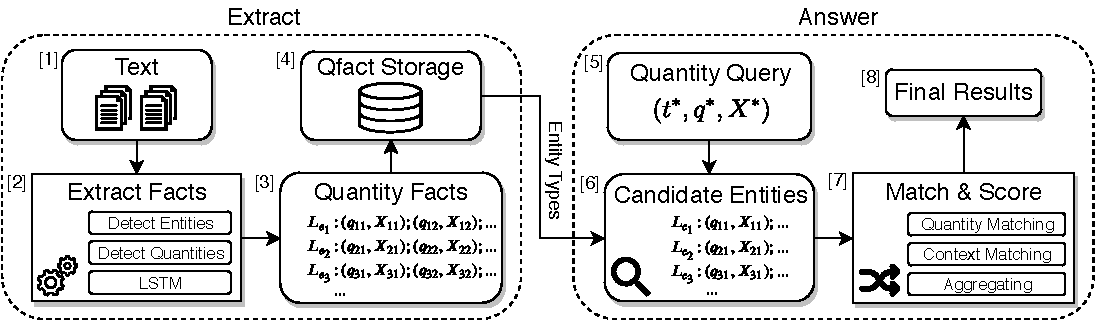
\includegraphics[width=1\textwidth]{figures/overview.pdf}
\caption{Overview of Qsearch.}
\label{fig:system}
\end{figure}
% what is the storage, how is it stored, and indexed 

\subsubsection{Extract.}  
We preprocess the text corpus (Block 1) to recognize
and disambiguate named entities 
%using the AIDA \cite{DBLP:conf/emnlp/HoffartYBFPSTTW11} system,
%which links named entities to the YAGO knowledge base\cite{DBLP:conf/www/SuchanekKW07}. 
and link them to an external knowledge base (KB). We also identify mentions of quantities in the text and normalize them into standard units. 
Subsequently, we run a deep neural network to extract Qfacts from the preprocessed text (Block 2). We learn and employ a specifically designed
Long Short Term Memory (LSTM) network, which will be described in Section \ref{sec:extract}. 

Extracted Qfacts are organized and grouped by their named entities, such that each individual entity $e_i$ is mapped to a list of quantities and related contexts $L_{e_i} = \{(q_{i1},X_{i1}),(q_{i2},X_{i2}),... \}$ (Block 3).
All extracted Qfacts are stored in a data repository (Block 4, 
based on Elasticsearch in our implementation), where entities are linked to their semantic types from the KB.
%We use AIDA \cite{DBLP:conf/emnlp/HoffartYBFPSTTW11} for entity linking, YAGO \cite{DBLP:conf/www/SuchanekKW07} for entity typing, and ElasticSearch as a storage engine.



\subsubsection{Answer.}
We answer incoming Qqueries by matching them against
the Qfacts from the \textit{Extract} stage. 
For a Qquery $(t^*,q^*,X^*)$ (Block 5), we first apply 
an entity-type filter, eliminating entities with the wrong type. 
This results in a set of candidate entities $\mathcal{C} = \{c_1,c_2,...\}$ (Block 6) satisfying the type constraint $t^*$, along with their quantity-context pairs $\{L_{c_1},L_{c_2},...\}$. 
In Block 7, we discard all candidate answers 
%with quantity-context pairs $(q,X) \in L_c$ 
that do not satisfy the quantity condition $q^*$.
Finally, we compute a matching score for each candidate entity $c \in \mathcal{C}$ based on the contexts $X$ in the
quantity-context pairs $L_c$, using a statistical language model
or a text embedding method, which will be described in Section \ref{sec:match}. The candidate entities are ranked by their scores and returned to the user (Block 8). 

In the following Sections
\ref{sec:extract} and \ref{sec:match}, we discuss in detail the
 Qfact extraction model and the matching and answering model, 
respectively.

%In the remainder of this section, we discuss how each candidate entity is scored in Block 7.

\section{Quantity Fact Extraction From Text}
\label{sec:extract}
In this section, we describe our method for extracting Qfacts from natural language text.
%which are then used to answer quantity queries. 
At the core of our solution is a deep-learning neural network for sequence tagging, running on individual sentences. 
%Moreover, we suppose that the input sentence is pre-processed by detecting entities and quantities in advance.

\subsubsection{Input Preprocessing.} In the first step, we preprocess the input text corpus by detecting entities and quantities appearing in each individual input sentence.  
We perform Named Entity Disambiguation (NED) 
using the AIDA \cite{DBLP:conf/emnlp/HoffartYBFPSTTW11} system,
which links named entities to the YAGO knowledge base\cite{DBLP:conf/www/SuchanekKW07}. To achieve a better detection quality, we run NED on a per-document instead of per-sentence basis.
For detecting quantities, we make use of the Illinois Quantifier \cite{DBLP:journals/tacl/RoyVR15}, a state-of-the-art tool for 
recognizing numeric quantities in text, along with some hand-crafted rules (e.g., regular expressions). 
Subsequently, each identified quantity is replaced by a placeholder \textit{``\_QT\_''}. 
\begin{example}
\label{ex:3}
Input and output of this preprocessing step look as follows:
{\small
\begin{align*}
\textit{sentence} &\ |\ \textit{BMW i8 has price of 138k Euros in Germany and range from 50 to 60 km on battery .} \\
\textit{preproce}&\textit{ssed}\ |\ \overbrace{\textit{BMW i8}}^{\mathclap{e_1=\textit{<KB:BMW\_i8>}}}\textit{ has price of }\underbrace{\textit{\_QT\_}}_{\mathclap{q_1=\textit{(138.000,\euro,appr.)}}}\textit{ in }\overbrace{\textit{Germany}}^{\mathclap{e_2=\textit{<KB:Germany>}}}\textit{ and range } \underbrace{\textit{\_QT\_}}_{\mathclap{q_2=\textit{(50-60,km,interval)}}}\textit{ on battery .}  \tag*{\qed}
\end{align*}
%%%GW:  Q - uppercase - is a Qfact. For quantity alone, we should use q - lowercase.
}
\end{example}
\subsubsection{Sequence Tagging Model.} In the second step, we aim to extract complete Qfacts from the preprocessed sentences. 
For each quantity detected in the previous step, we want to identify the entity to which it refers
and the relevant context tokens that express the entity-quantity relation.
\begin{example} 
Consider the preprocessed sentence in Example \ref{ex:3}. If we use the first quantity $q_1 = \textit{(138.000, \euro, approximate)}$
as the input's pivot, 
we want to obtain the output $e(q_1) = e_1 = \textit{<KB:BMW\_i8>}$ and $X(q_1)=\{\textit{price, Germany}\}$. 
Analogously, with $q_2 = \textit{(50-60, km, interval)}$ as pivot,  the desired output is 
$e(q_2)= e_1 = \textit{<KB:BMW\_i8>}$ and $X(q_2)=\{\textit{range, battery}\}$. \qed
\end{example}
We formalize this task as a sequence labeling problem as follows.
\begin{task}[Quantity Fact Extraction]
Given a preprocessed sentence $S$ with the set of detected entities $\mathcal{E} = \{e_1,e_2,...\}$, the set of detected quantities $\mathcal{Q} = \{q_1,q_2,...\}$ and a selected pivot quantity of interest $q_i \in \mathcal{Q}$, the task of quantity fact extraction is to label each token of the sentence with one of the following tags: (i) \textit{<E>}, for denoting the entity that $q_i$ refers to; (ii) \textit{<X>}, for denoting the context tokens that relate $q_i$ and its entity; and (iii) \textit{<O>}, for all other tokens.
\end{task}
\begin{figure}[t]
\centering
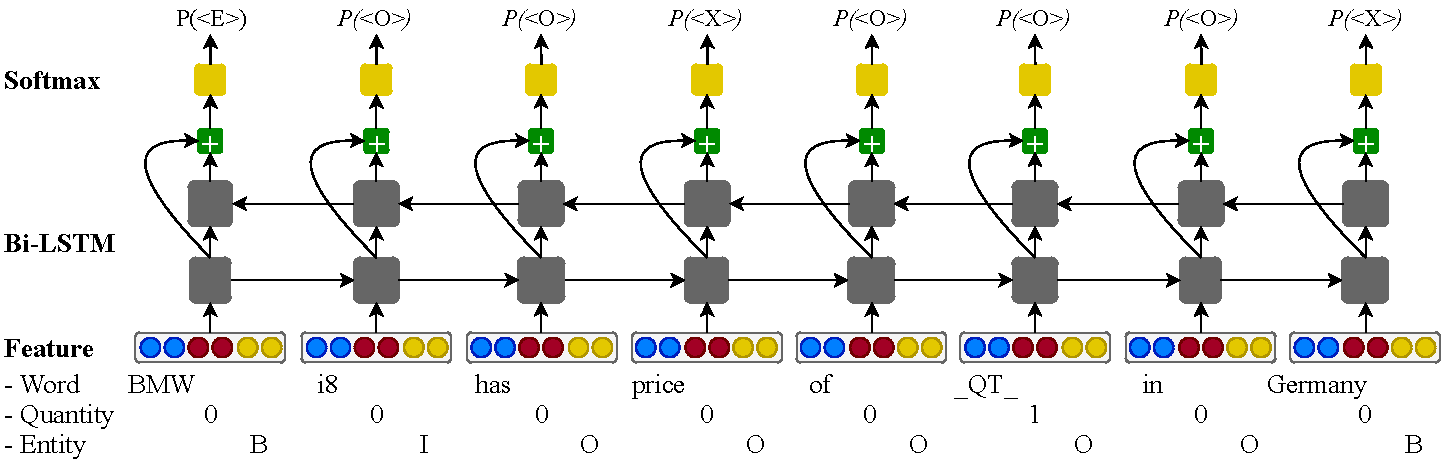
\includegraphics[width=1\textwidth]{figures/neural.pdf}
\caption{The Qfact extraction model used by Qsearch.}
\label{fig:neural}
\end{figure}
Our problem resembles the Semantic Role Labeling task \cite{DBLP:journals/coling/GildeaJ02}, which is typically addressed by
Conditional Random Fields (CRFs)
or Long Short Term Memory (LSTM) models. 
Figure \ref{fig:neural} depicts the bi-directional LSTM model 
that we devised for this task, inspired by prior work \cite{DBLP:conf/acl/HeLLZ17a}.
 Other models for sequence labeling (e.g., \cite{DBLP:conf/acl/ZhouX15, DBLP:conf/emnlp/FitzGeraldTG015})
could be easily incorporated as well. 
Our labeling network consists of three layers: Input Features, Bi-LSTM, and Softmax. 
While this general architecture is close to any other LSTM model, the most unique point here is the input representation,
as described next.

\subsubsection{Input Features.} Each token of the preprocessed input sequence is represented as the concatenation of three input feature vectors:
\begin{enumerate}[label=(\it\roman*)]
\item \textit{Word}: We include word embeddings as an input feature, which enables the neural model to 
generalize to different words having similar meanings.
In our implementation, we use Glove \cite{DBLP:conf/emnlp/PenningtonSM14} precomputed embeddings.
\item \textit{Quantity}: We provide the position of the 
pivot quantity to the model as input. 
When sentences contain multiple quantities (which is a relatively frequent case), our model operates
one quantity at a time and we re-run the model for different quantities.
%which resembles the Semantic Role Labeling task, where the verbs are passed into the input instead of the quantities.
\item \textit{Entity}: We also provide information about the recognized entities as input to the neural model. 
As entities often span multiple tokens, we employ the BIO tagging mechanism \cite{DBLP:conf/acl-vlc/RamshawM95}, where a tag \textit{B} is used for tokens at the beginning of an entity name,
\textit{I} for tokens inside the name, and \textit{O} for other tokens. 
With this representation, the output of the model only needs to tag the first token of a multi-word entity name with \textit{<E>}, 
and subsequent tokens are tagged with \textit{<O>}. Figure \ref{fig:neural} shows an example: \textit{``BMW i8''} is chosen as the entity 
connected with the pivot quantity; only the first token \textit{``BMW''} is tagged as \textit{<E>} in the output.
\end{enumerate}

\subsubsection{Output Constrained Decoding.} The output of the model are the probabilities of each token word in the input belonging to each of the three tags \textit{<E>}, \textit{<X>} and \textit{<O>}, produced by the Softmax layer. 
In neural models, usually the tag with the highest score will be assigned to each token word.
%which results in the highest probability of the whole tag sequence. 
However, this standard technique would not take into account the dependencies between output tags, and hence might give us an invalid tag sequence. To solve this issue, we impose the following two constraints on the output of the model at decoding time, and find the most probable tag sequence satisfying them: \textit{(i)} only one tag \textit{<E>} can appear in the output
(namely, for the one entity to which the pivot quantity refers);
and \textit{(ii)} that tag \textit{<E>} has to be at the start token of an entity name. 


To find the most probable tag sequence, we use Dynamic Programming to decode from left to right. Specifically, we compute subsequences of tags $\textit{Seq}_{i,j,k}$ for every $i \in \{1..n\}$ ($n$ is the sentence length)$; j \in \{\textit{<E>}, \textit{<X>}, \textit{<O>}\};$ and $k \in \{0, 1\}$. Here, $\textit{Seq}_{i,j,k}$ denotes tag subsequence with the highest probability for tokens from position $1$ to position $i$, where the tag of token at position $i$ is $j$, and the subsequence contains $k$ \textit{<E>} tags.
Note that the probability of a tag subsequence is computed as the product of the probabilities of its constituent tags. 
The final tag sequence can be derived at $i = n$.

%The final tag sequence can be derived at position $i = n$.

%We compute subsequence of tags from position 0 to i, denoted as  $\textit{Seq}_{i,j,k}$ where $i \in \{1..n\}; j \in \{\textit{<E>}, \textit{<X>}, \textit{<O>}\};$ and $k \in \{0, 1\}$. Here, $\textit{Seq}_{i,j,k}$ represents that the tag of token at position $i$ is $j$ and $k$ is interpreted as the tag subsequence with the highest probability for tokens from position $1$ to $i$.
%where the tag of token at position $i$ is $j$, and the subsequence contains $k$ \textit{<E>} tags.


\subsubsection{Distant Supervision Training.} As training data is an important factor but difficult to obtain, and manual labeling 
at scale is too 
expensive, we employ distant supervision to generate training data for the Qfact extraction model.
We use unsupervised, pattern-based Open Information Extraction (Open IE) to overlay an n-tuple structure
(with triples or higher-arity tuples) 
on the input text. 
We employ the OpenIE4 tool \cite{DBLP:conf/ijcai/Mausam16} to this end, and then use its output tuples
to generate training data. This process consists of two steps:\\

\noindent \textit{- Step 1: Capture information areas:} We define an \textit{information area} as a subset of tokens from a sentence, which presents complete information about a fact.
We run Open IE on the \textit{unprocessed} sentence to detect all possible tuples expressed by the text. 
Each of these tuples has a confidence score; to ensure the quality of the generated training samples, 
we only keep tuples having a confidence score of at least 0.9. 
Each of the selected tuples corresponds to an information area.
\begin{example} Consider the unprocessed sentence in Example \ref{ex:3}, suppose the following tuples are extracted by Open IE: (1): \textit{(BMW i8; has; price of 138k Euros; in Germany)$^{0.95}$}, (2): \textit{(BMW i8; has; range from 50 to 60 km on battery)$^{0.9}$}, (3): \textit{(BMW i8; has; price of 138k Euros)$^{0.8}$}, (4): \textit{(BMW i8; has; range from 50 to 60 km)$^{0.5}$}, and (5): \textit{(BMW i8; has; price)$^{0.1}$}. We only keep high-confidence tuples (1) and (2), which contain complete information. 
Then the following information areas are chosen for training:
{\small
\begin{align*}
\mathrlap{\underbracket{\phantom{\textit{BMW i8 has }}}_{\textit{(2)}}} \overbracket{\textit{BMW i8 has price of 138k Euros in Germany}}^{\textit{(1)}} and \underbracket{\textit{range from 50 to 60 km on battery}}_{\textit{(2)}} . \tag*{\qed}
\end{align*}
}
\end{example}
\noindent \textit{- Step 2: Transform infomation areas into training samples:} We map the information areas obtained in Step 1 with entities and quantities detected from the preprocessing phase:
{\small
\[
 \mathrlap{\underbracket{\phantom{\textit{<KB:BMW\_i8> has }}}_{\textit{(2)}}} \overbracket{\textit{<KB:BMW\_i8> has price of \_QT\_}_{(1)} \textit{in <KB:Germany>}}^{\textit{(1)}} and \underbracket{\textit{range \_QT\_}_{(2)} \textit{on battery}}_{\textit{(2)}} . \tag*{\qed}
\]
}
With this mapping, information areas yield training samples for the neural network. 
We apply conservative filters so that this self-training process minimizes spurious samples.
First, we keep only information areas that contain exactly one quantity \textit{\_QT\_}, the pivot quantity. 
Second, since English sentences tend to express quantity information in active voice, 
the entity connected to the pivot quantity should appear in the first argument (subject) of the Open IE tuple. 
For instance, information area (1) has two entities \textit{<KB:BMW\_i8>} and \textit{<KB:Germany>};
we choose the former as the one to which quantity \textit{\_QT\_$_{(1)}$} refers. 
Finally, we discard all information areas where the subject of the Open IE tuple contains more than one entity.

At this point, for each information area, we have a quantity and a unique entity to which it refers. 
The context between them is determined from the remaining tokens in the information area based on their Part-of-speech (POS) tags. 
We allow only the following POS patterns to form the context: noun (NN*), verb (VB*), adjective (JJ*), adverb (RB*), and 
foreign  word (FW, to capture out-of-vocabulary names). 
We also use pre-defined stopwords to remove uninformative tokens from the context. 
The resulting Qfact, along with the \textit{<E>,<X>,<O>} tags for its token sequence, becomes a positive training sample.
%Furthermore, to prevent the tagging model from being overly optimistic, we also take into account negative training samples, 
As negative training samples, we collect all information areas where no entity could be identified to relate with the
pivot quantity, i.e., all tokens are tagged as \textit{<O>}.


%{\tt\color{red} GW: need to say more about the actual training - size of training data, which 
%software library, batch size, epoch size, learning rate etc. !!!!!!!!!!}

 
%!TEX root = ../main.tex
\section{Candidate Fact Matching Model} 
\label{sec:match}
This section describes our method to answer Qqueries from the extracted Qfacts. To this end, each Qfact is assigned a score denoting its relevance to the given Qquery.

\subsubsection{Query Parsing.} 
%We implemented a simple parser to transform the user queries into the Qquery format. 
Input questions are mapped into Qqueries by a rule-based parser for recognizing answer type and quantity condition; all other tokens (except stopwords) are included in the query context. The parser uses a dictionary of YAGO types and a dictionary of quantity units. An alternative to this rule-based technique would be to apply the same neural extraction method to questions that we have used to extract Qfacts from text. However, the questions are easier to handle, and the rule-based parser works well. 

\begin{task}[Quantity Fact Scoring] Given Qquery $\mathcal{Y} = (t^*,q^*,X^*)$ and Qfact $\mathcal{F} = (e,q,X)$, compute a distance score $d(\mathcal{F}, \mathcal{Y})$ reflecting the relevance of $\mathcal{F}$ regarding $\mathcal{Y}$.
\end{task}
Without loss of generality, we assume that a lower score denotes a better fact.
%As mentioned in Section \ref{sec:framework}, 
$\mathcal{F}$ should be a high-ranked answer for $\mathcal{Y}$ iff the following three conditions hold:
(1) $e$ is an entity of type $t^*$, 
(2) $q$ satisfies $q^*$, and (3) $X$ is a good (approximate) match for $X^*$.

%\begin{task} [Quantity Fact Retrieval] Given a quantity query $\mathcal{Q}$ and a set of candidate quantity facts $\mathbb{F} = \{\mathcal{F}_1,\mathcal{F}_2,... \}$, return a ranked list of facts $\mathbb{F}_i \subset \mathbb{F}$
%\end{task}
\subsubsection{Entity - Type Matching.} We only consider the Qfact $\mathcal{F}$ if the entity $e$ has type $t^*$. Since the entities from text are linked to an external knowledge base, we make use of the type information from the KB to filter out unsuitable facts for $\mathcal{Y}$. %This is done in Block 6 of the Qsearch overview (Figure \ref{fig:system}).

\subsubsection{Quantity Matching.} We also discard $\mathcal{F}$ if $q$ does not satisfy $q^*$. This is the case when either (1) the units of $q$ and $q^*$ relate to different concepts (e.g. \textit{km} (length) vs. \euro (money)) and are thus incomparable; or (2) their values (after conversion to the same unit) do not match the comparison operator of $q^*$. Since quantity matching is not the focus of our paper, we apply a simple matching method as follows. First, we use hand-crafted rules for unit conversions, re-scaling if needed (e.g., for kilo, mega, etc.), and value normalization. Second, we turn the quantity value into an interval based on its resolution. For example, when the query is about approximate matches, a quantity value $v$ is smoothed into the interval $[v-\delta, v+\delta]$ with a configuration parameter $\delta$. In experiments, we set $\delta$ to 5\% of $v$. A comparison is considered a match when the two intervals overlap, and their units (after conversion and re-scaling) match.

\subsubsection{Context Matching.} If the Qfact $\mathcal{F}$ satisfies the above two constraints, we will consider the similarity between the query context $X^*$ and the fact context $X$. We propose to use the following two approaches for measuring the context relevance: a \textit{probabilistic} and an \textit{embedding-based} approach.\\

\noindent \textbf{Probabilistic Ranking Model.} We adopt the Kullback-Leibler (KL) divergence between the query context $X^*$ and the fact context $X$, which is typically used in statistical language models \cite{DBLP:journals/ftir/Zhai08}. The scoring function is defined as follows:
\begin{align*}
d(\mathcal{F}, \mathcal{Y}) = \textit{KL}(X^*, X) &= H(X^*, X) - H(X^*) \\ &\equiv H(X^*, X) 
= -\sum_{w \in \mathcal{V}} P(w|X^*)\,\log P(w|X)
\end{align*}
where $\mathcal{V}$ is the word vocabulary, $H(X^*)$ is the entropy of $X^*$; $H(X^*, X)$ is the cross entropy between $X^*$ and $X$; and $\equiv$ indicates rank equivalence
(i.e., preserving order). 
Since we are only interested in ranking fact contexts in response to a query context, we can omit $H(X^*)$. The word probability $P(w|X^*)$ for the query context is estimated using Maximum Likelihood Estimation (MLE) on an expanded version $X^*_E$ of $X^*$ as:
\[P(w|X^*) = count(w \in X^*_E)/|X^*_E|\]
To expand a query context, we resort to WordNet \cite{Miller:1995:WLD:219717.219748} and add all synonyms of the context words to it. For the fact context, we estimate the word probability $P(w|X)$ using Jelinek-Mercer smoothing 
%to avoid zero probabilities
 as:
\[P(w|X) = (1 - \lambda) \times count(w \in X)/|X| + \lambda \times P(w|B)\]
This linearly combines the MLE from the fact context $X$ with the MLE obtained from a background corpus $B$. The smoothing parameter $\lambda$ (set to $\lambda=0.1$ in our system) controls the influence of the background corpus on the probability estimate. We construct the background corpus $B$ from all sentences of the entire text corpus that contain at least one quantity (total 39M sentences in our data). \\


%Since these two estimates are very sparse, before calculating, we expand $X^*$ and $X$ using an external resource. Moreover, a smoothing method is applied to avoid zero counts.
%\thinh{Should explain more? which resource, how to expand, which smoothing method.}

\noindent \textbf{Embedding-based Ranking Model}: 
We observed on our data that the query context $X^*$ is often shorter than the fact context $X$, since sentences are often more verbose than the typically short queries. Hence, to measure the distance score of $X$ with regard to $X^*$, we can match tokens between $X^*$ and $X$ using word embedding similarity as follows:
\[d(\mathcal{F}, \mathcal{Y}) = {\bigg(\sum\limits_{u \in X^*} \min\limits_{v \in X}(dist(u,v))\bigg)}/{|X^*|}\]
where $dist(u,v) \geq 0$ is the semantic distance between two words $u$ and $v$ estimated from their pre-computed word embedding vectors \cite{DBLP:conf/emnlp/PenningtonSM14}. 
We use cosine distance in the Qsearch implementation, re-scaled for normalization to [0,1]. 
In the above equation, 
we map each word of query context $X^*$ to its closest word in the fact context $X$ in the embedding space. This scoring formula gives the same weight to every token in the query context $X^*$, which might be misleading, since they could have a different degree of importance.
%Therefore, to increase the impact of more important words and to reduce the role of less %important ones in $X^*$, 
This issue is overcome by giving higher weight to important words and lower weight
to uninformative words, using
%we use 
the following distance function:
\[d(\mathcal{F}, \mathcal{Y}) = \frac{\sum\limits_{u \in X^*} W(u)\min\limits_{v \in X}(dist(u,v))}{\sum\limits_{u \in X^*}W(u)} + 1\]
where $W(u) \geq 0$ is the importance weight of word $u$. 
There are several weighting functions that can be used for $W$ (e.g., \textit{inverse document frequency (idf)}, \textit{term strength}, etc.); we use Robertson’s \textit{idf}\cite{DBLP:journals/jd/Robertson04}. 
We call the above formula the 
\textit{directed embedding distance}, $ded(X^* \rightarrow X)$,
between query and fact contexts.

$ded(X^* \rightarrow X)$ describes how well each word in $X^*$ matches with some other word in $X$, but in many cases it fails to reflect the match between their meaning. The presence of a single word in the fact context $X$ can totally change its meaning. Consider, as a concrete example, the two contexts $X^*=\{\textit{net, worth}\}$ vs. $X = \{\textit{negative, net, worth}\}$. Hence, our idea is to penalize the relevance score with an amount proportional to the directed embedding distance between $X$ and $X^*$.
Specifically, we define the \textit{context embedding distance ($ced$)} that implements this idea:
\begin{align*}
&d(\mathcal{F}, \mathcal{Y}) = ced(X^*, X) = ded(X^* \rightarrow X) \times ded(X \rightarrow X^*)^\alpha \\
=& \Bigg( \frac{\sum\limits_{u \in X^*} W(u)\min\limits_{v \in X}(dist(u,v))}{\sum\limits_{u \in X^*}W(u)} + 1 \Bigg) \times \Bigg( \frac{\sum\limits_{u \in X} W(u)\min\limits_{v \in X^*}(dist(u,v))}{\sum\limits_{u \in X}W(u)} +1 \Bigg)^\alpha 
\end{align*}
Intuitively, our $ced$ measure is the product of two components: (1) $ded(X^* \rightarrow X)$ captures how well query context tokens match with fact context, and (2) $ded(X \rightarrow X^*)$ reflects how much additional terms in $X$ shift its meaning, and hence, should be penalized. Parameter $\alpha \in [0,+\infty)$ controls how much the penalty scaling affects the total score.

\begin{example} Consider the Qquery context $X^* = \{\textit{gross, domestic, product}\}$ and two Qfact contexts $X_1 =$ \{\textit{gross, national, product}\}, $X_2 =$  \{\textit{gross, domestic, product, capita}\}. While we are more inclined to $X_1$ than $X_2$, the directed embedding distance $ded(X^* \rightarrow X_2)$ has a slightly better score than $ded(X^* \rightarrow X_1)$, as it does not penalize the word \textit{``capita''}
(which indicates that the GDP is per capita, not the total GDP). 
In contrast, $ded(X_1 \rightarrow X^*)$ is lower than $ded(X_2 \rightarrow X^*)$ (since \textit{``national''} is close to \textit{``domestic''}), preferring $X_1$ over $X_2$ with regard to $X^*$, which results in the desired ranking based on the context embedding distance $ced$. \qed
\end{example}

\subsubsection{Entity Scoring.} The output of Qsearch is a ranked list of entities from matching Qfacts with the Qquery. 
%In Block 7 of the system overview (Figure \ref{fig:system}), we give 
We assign a score for each candidate entity 
%$c \in \mathcal{C}$ based on its quantity-context pairs $L_{c} = \{(q_{c1},X_{c1}),%(q_{c2},X_{c2}),... \}$. Note that after filtering based on the quantity condition, we only need %to consider context matching.
based on one of the above context distance models and
aggregating over the entity's quantity-context pairs as follows:
\[\textit{score}(c \in \mathcal{C}, \mathcal{Y}) = \min\limits_{(q, X) \in L_c} d(\mathcal{F}=(c,q,X), \mathcal{Y})\]
where $d(\mathcal{F}, \mathcal{Y})$ is either the Kullback-Leibler divergence $\textit{KL}(X^*, X)$ or the context embedding distance
$ced(X^*,X)$.
So when the same candidate entity appears in multiple Qfacts, we pick the best-scoring
Qfact context distance.
%Put differently, we rank candidate entities based on their best fact context, i.e., the one %achieving the lowest distance to the query context.


%!TEX root = ../main.tex

\section{Evaluation}
We run experiments on a Linux machine with 80 CPU cores, 500GB RAM, and 2 GPUs. To evaluate Qsearch, we perform an intrinsic evaluation of our {\em Qfact extraction model} and an extrinsic evaluation of the {\em end-to-end Qsearch system}.
\subsubsection{Dataset.} All experiments use a large collection of news articles, compiled from two real world datasets: the \textit{STICS} project \cite{DBLP:conf/sigir/HoffartMW14} with news from 2014 to 2018, 
and the \textit{New York Times} archive
\cite{nyt}
 %5843811 + 1765538
with news from 1986 to 2008.
In total, our corpus consists of 7.6M documents.
 
\subsection{Intrinsic Evaluation of the Quantity Fact Extraction Model}
%We conduct intrinsic evaluation to examine the quality of our Qfact extraction model of the %\textit{Extract} stage.
\subsubsection{Training setup.}
We implemented the  LSTM network using Theano library,
largely following \cite{DBLP:conf/acl/HeLLZ17a} for the training 
configuration: using Adadelta with $\epsilon = 1e^6$ and $\rho = 0.95$;  \textit{lstm\_hidden\_unit = 300}; \textit{rnn\_dropout\_prob = 0.1}; \textit{batch\_size = 100}.

We extracted training samples from the corpus using the distant-supervision technique as described in Section \ref{sec:extract} and conducted the training process with different settings. 
In the \textit{General} setting, we use all available training data
of 3.2M training samples, where we maintain the ratio 3:1 between the number of positive and negative samples.
We also train our model for three other 
\textit{measure-specific} settings, where only a subset of the training samples is used. In particular, we classify training samples into different categories based on the quantity unit. For example, training samples containing quantities with unit \textit{Kilometer} or \textit{Meter} are chosen to train the model in the \textit{Length} setting, while the ones with unit \textit{US dollar}, \textit{Euro}, etc. are picked for the \textit{Money} setting. 
Among many such categories, we selected the three most prevalent measures \textit{Money}, \textit{Percentage} and \textit{Length}, containing 307K, 235K and 41K training samples, respectively (also with ratio 3:1  between positive and negative samples). 
%to train the corresponding models. 
The trained models are then applied to the entire corpus to extract more Qfacts. 
%Note that the input for the trained models should be compatible with their trained settings.

\subsubsection{Performance of Extraction model.}
As the test data does not have any ground-truth labels, 
we randomly selected 100 samples that contain at least two entities from the output tag sequences, for each training model, and manually assessed their validity.
\begin{table}[t]
\centering
\caption{Evaluation of Qfact extraction model of Qsearch on different settings.}
\begin{tabular}{c |r r r|r r r|r r r|r r r} \midrule
 \multirow{2}{*}{\textbf{Tag}} & \multicolumn{3}{c}{\textbf{Length}} & \multicolumn{3}{|c}{\textbf{Money}}  & \multicolumn{3}{|c}{\textbf{Percentage}}  & \multicolumn{3}{|c}{\textbf{General}} \\
 \cmidrule{2-13}
 & \textit{~Prec.} &  \textit{~~~Rec.} & \textit{~~~~~F1~} & \textit{~Prec.} &  \textit{~~~Rec.} & \textit{~~~~~F1~} & \textit{~Prec.} &  \textit{~~~Rec.} & \textit{~~~~~F1~} & \textit{~Prec.} &  \textit{~~~Rec.} & \textit{~~~~~F1~} \\
 \midrule
\textbf{E} & 0.860 & 0.860 & 0.860 & 0.850 & 0.850 & 0.850 & 0.794 & 0.770 & 0.782 & 0.882 & 0.820 & 0.850 \\
\textbf{X} & 0.650 & 0.849 & 0.736 & 0.717 & 0.844 & 0.776 & 0.659 & 0.827 & 0.734 & 0.728 & 0.713 & 0.721 \\
\textbf{O} & 0.958 & 0.886 & 0.920 & 0.942 & 0.886 & 0.913 & 0.947 & 0.888 & 0.917 & 0.895 & 0.906 & 0.900 \\
 \midrule
\textbf{Macro-avg.} & 0.823 & 0.865 & 0.839 & 0.836 & 0.860 & 0.846 & 0.800 & 0.828 & 0.811 & 0.835 & 0.813 & 0.824 \\
 \midrule
\end{tabular}
\label{table:extract_quality}
\end{table}

We evaluate the quality of the three output labels \textit{<E>}, \textit{<X>} and \textit{<O>} by three measures: \textit{Precision}, \textit{Recall}, and \textit{F1 score}.
The results are shown in Table \ref{table:extract_quality}. 
We observe that all training models perform very well on entity tagging with more than 85\% \textit{F1 score}. 
%This assures that our model can efficiently identify the referred entity for a given quantity. 
%The results also show that the extraction models can capture around 70\% of correct context %tokens of the Qfacts.
We also see that the measure-specific training variants for Length and Money
have slight advantages.

%Moreover, the extraction model also achieves at least 90\% accuracy in identifying \textit{<O>} tag, which helps to reduce the noisy candidates for answer generation step. 

%%%%%%%%%%%%%%%%%%%%%%%%%%%%%%%%%%%%%%%

\subsection{Extrinsic Evaluation of the End-to-End Qsearch System}
We performed the extrinsic evaluation of Qsearch 
on a benchmark of 100  quantity queries, collected by crowdsourcing
and covering four domains: \textit{Finance}, \textit{Transport}, \textit{Sports} and \textit{Technology}. 
These queries capture a wide diversity of measures and units as well as variety in query formulations
(e.g., phrases for the comparison operators); see Table~\ref{table:query_stat}. 
%Conditional phrases are also varies widely, e.g., less than, above, over, etc. 
Anecdotal examples of user queries and their answers produced by Qsearch are shown in Table~\ref{table:example_qa}.
We also considered queries from the QALD-6-task-3 statistical QA benchmark \cite{DBLP:conf/esws/UngerNC16},
but out of total 150 training and test queries, we found only 6 with quantity conditions (as opposed to simpler property lookups).

In this evaluation, we use the Qfact extraction model trained under the \textit{General} setting, as it generalizes to different measures and units.
%Here, we discuss the performance of our system which is built upon the facts extracted from the proposed quantity fact %extraction model trained under the \textit{``General''} setting. 
%!TEX root = ../main.tex

\begin{table}[t]	
	\centering
	\small
	\caption{Statistics of benchmark queries from each domain.}
	\begin{tabular}{l| c c c c l } \midrule
		\multirow{2}{*}{\textbf{Domain}} & \multicolumn{5}{c}{\textbf{Distribution of queries based on unit of quantity}} \\
		\cmidrule{2-6}
		    & \textit{~Money~} & \textit{~Length~} & \textit{~Percentage} & \textit{~Others~}~ & \textit{~Examples for Others}\\ \midrule
		Finance &  76 \% & - & 12 \% & 12 \%~   & ~no. of sales, albums, etc.\\ 
		Transport &   4 \% & 32 \% & -& 64 \%~    &~MPG, mph, horsepower, etc.  \\  
		Sports &   8 \% & 32 \% & -&60 \%~ &  ~sec, years, kg, no. of medals, etc.  \\  
		Technology &  20 \% & 20 \% & 8 \% & 52 \% ~& ~megapixels, Watt, mAh , etc. \\ \midrule 
	\end{tabular}
	\label{table:query_stat}
\end{table} 
%!TEX root = ../main.tex
\begin{table}[t]
	\caption{Anecdotal examples of quantity queries and results from Qsearch.}	
	\small	
	\begin{tabular}{p{.2\textwidth} p{.8\textwidth}} 	 \hline
		Domain & Query \\ \hline
		Finance & \textbf{Q1:} Coal companies with more than 200 Million dollar annual profit\\ 
		Transport & \textbf{Q2:} Sport utility vehicles with engine power at least 150 horsepower \\  
		Sports & \textbf{Q3:} Sprinters who ran 100 meter in less than 10 seconds  \\  
		Technology & \textbf{Q4:} Digital cameras with focal length of lens more than 18 mm\\ \bottomrule 
	\end{tabular}
	\small
	\begin{tabular}{p{.075\textwidth} p{.15\textwidth} p{.775\textwidth}} 
	 \hline
		Query & Result & Corresponding Sentence \\ \hline
		Q1& Duke Energy & Duke Energy had revenue of \$ 23.9 billion and profit of \$ 1.9 billion last year.\\ \hline
		
		Q2 & Ford Escape & Its V-6 engine (the Escape is a four-cylinder) has 270 horsepower, 20 percent more than the Lexus RX330. \\ \hline
		Q3 & Andre Grasse & Andre De Grasse, a 20-year-old from Markham, Ont., has run the 100 metre in under 10 seconds three times this year. \\ \hline
		Q4 & Nikon D7100 & For example, the D7100 can be found in a kit with 18-140 mm and 55-300 mm lenses , so you'll want to use the 55-300 mm and zoom in to 300 mm. \\
		\bottomrule
	\end{tabular}	
	\label{table:example_qa}
\end{table}

\subsubsection{Setup.} 
For each Qquery, we consider top-10 results returned by Qsearch and evaluate 
their relevance and validity by judgements from crowd-workers (using Figure-Eight platform, formerly known as CrowdFlower).
The judges were shown the query, the top-10 entity answers, 
and the corresponding 10 sentences from which the answers were extracted. 
Each result was annotated  as \textit{relevant} or \textit{irrelevant} to the query based on the cue given in its corresponding sentence.
For each query, we collected three judgements and 
used the majority label as gold standard. Overall, we obtained a high inter-annotator agreement with Fleiss' Kappa value of 0.54.

\subsubsection{Baselines.} 
Although our Qsearch system produces entities as main result, we still want to compare it with standard search systems, which produce snippets. 
As there is no other system that can handle quantity queries with crisp entity answers, we use
search systems as baselines that produce text snippets as answers.
Specifically, we ran all benchmark queries on Elasticsearch, locally indexing all sentences of our news corpus,
and on Google web search retrieving the top-10 result snippets.
Elasticsearch uses a text-oriented state-of-the-art ranking model based on BM25.
%

The baselines were given certain advantages, to avoid that Qsearch could be viewed as an unfair competitor.
For Elasticsearch, we consider only sentences that contain an entity and a quantity. For the evaluation, we asked crowd-workers to annotate top-10 results, retrieved from Elasticsearch, as relevant or irrelevant based on whether they spotted a reasonable result for the quantity query.
To evaluate result snippets from Google search, we instructed annotators to be generous, as the result snippets are not well-formed sentences (but could be synthesized from
non-contiguous text segments with ellipses). For example, a text snippet that contains a correct entity and its quantity is considered relevant even if it also contains other entities or quantities. Such instructions to annotators give Google results an advantage because Qsearch results are considered relevant only if both entity and quantity are correctly extracted.
%For both Elasticsearch and Google, we evaluated the top-10 results, sentences or answer snippets, respectively.
%Crowd-workers were asked to annotate these as relevant or irrelevant based on whether they spotted
%a good result for the quantity query. 
%For Google Search, we  collect top-3 result snippets for each query. These snippets are manually annotated as %relevant if they mention a entity and the correct information satisfying the query. 
%For Google, as the result snippets are not well-formed sentences (but could be synthesized fromnon-contiguous text segments with ellipses), the annotators were instructed to be generous.

We also explored several state-of-the-art QA systems over linked open data:
Frankenstein
%\footnote{\url{http://frankenstein.qanary-qa.com/}}
\cite{DBLP:conf/www/SinghRBSLUVKP0V18},
QAnswer
%\footnote{\url{http://qanswer.eu/qa}}
\cite{DBLP:conf/www/DiefenbachMQLSM19},
Platypus
%\footnote{\url{http://askplatyp.us/}}
\cite{DBLP:conf/esws/TanonACS18},
AskNow
%\footnote{\url{https://asknowdemo.sda.tech/}}
\cite{DBLP:conf/esws/DubeyDSHL16}, 
Quint
%\footnote{\url{https://gate.d5.mpi-inf.mpg.de/quint/quint}}
\cite{DBLP:conf/emnlp/AbujabalRYW17},
SPARKLIS
%\footnote{\url{http://www.irisa.fr/LIS/ferre/sparklis/}}
\cite{DBLP:journals/semweb/Ferre17}.
%QAKiS\footnote{\url{http://qakis.org/qakis/index.xhtml}}~\cite{DBLP:conf/semweb/CabrioCAMLG12}.
None of these systems is geared for handling quantity questions, except SPARKLIS, however it can only process quantities without associated unit.
Moreover, their underlying KBs have poor coverage of quantities.
% (c.f., Table \ref{table:kg_stats})
%and thus fail to capture the semantic of quantitative facts. Due to these shortcomings, 
%all of the above mentioned LOD-based QA systems were unable to process our benchmark queries, and therefore we exclude them from further evaluation. 
They failed on almost all of our benchmark queries; so we excluded these systems from our comparative evaluation. 


\subsubsection{Performance of Qsearch. } 
Table \ref{table:performance_qsearch} shows the performance of Qsearch for the four domains and
for all 100 queries together, using the two variants of our ranking models:
KL divergence and context embedding distance ($ced$).
For $ced$ we empirically tune the parameter $\alpha = 3$  based on results from 10
validation queries
disjoint from the 100 test queries. 
We report three metrics: \textit{Precision@k}, \textit{Hit@k} and \textit{Mean-Reciprocal-Rank (MRR)}, 
macro-averaged over queries. 
We do not discuss metrics like Recall or MAP, as these would require exhaustively annotating a huge pool
of candidate answers.

\begin{table}[t]
\caption{End-to-end evaluation of Qsearch.}
\centering
\begin{tabular}{l |cc|cc|cc|cc| cc } \midrule
 \multirow{2}{*}{\textbf{~Metric~~}} & \multicolumn{2}{c}{\textbf{Finance}} & \multicolumn{2}{|c}{\textbf{Transport}} & \multicolumn{2}{|c}{\textbf{Sports}} & \multicolumn{2}{|c}{\textbf{Technology}} & \multicolumn{2}{|c}{\textbf{ All}} \\
 \cmidrule{2-11}
	&  \textit{~KL-div.~}&   \textit{~Emb.~} &  \textit{~KL-div.~} & \textit{~Emb.~} &   \textit{~KL-div.~}&   \textit{~Emb.~} &  \textit{~KL-div.~} & \textit{~Emb.~} &  \textit{~KL-div.~} & \textit{~Emb.~} \\
\midrule
\textbf{Pr.@1} & 0.720 & 0.800 & 0.480 & 0.600 & 0.560 & 0.680 & 0.640 & 0.680 & 0.600 & 0.690  \\
\textbf{Pr.@3} & 0.667 & 0.747 & 0.480 & 0.480 & 0.507 & 0.587 & 0.627 & 0.653 & 0.570 & 0.617 \\
\textbf{Pr.@5} & 0.632 & 0.672 & 0.412 & 0.412 & 0.480 & 0.528 & 0.550 & 0.624 & 0.519 & 0.559  \\ 
\textbf{Pr.@10} & 0.604 & 0.608 & 0.333 & 0.379 & 0.412 & 0.432 & 0.500 & 0.547 & 0.462 & 0.492 \\ 
\midrule
\textbf{Hit@3} & 0.880 & 0.920 & 0.760 & 0.760 & 0.760 & 0.800 & 0.840 & 0.880 & 0.810 & 0.840 \\
\textbf{Hit@5} & 0.880 & 0.960 & 0.760 & 0.760 & 0.920 & 0.840 & 0.840 & 0.920 & 0.850 & 0.870 \\ 
\midrule
\textbf{MRR} & 0.792 & 0.870 & 0.621 & 0.678 & 0.685  & 0.746 & 0.747 & 0.783 & 0.711 & 0.769 \\
 \midrule
\end{tabular}
\label{table:performance_qsearch}
\end{table}

%\textbf{Pr.@1} & 0.240 & 0.720  &  0.800 & 0.240& 0.480  &  0.600 & 0.200 & 0.560 & 0.680 & 0.320 & 0.640  &  0.680  \\
%\textbf{Pr.@3} & 0.307 &  0.667 & 0.747 & 0.213 & 0.480 & 0.480  & 0.213 & 0.507  & 0.587 & 0.347 & 0.627  &  0.653  \\
%\textbf{Pr.@5} & 0.248 & 0.632  & 0.672 & 0.184 & 0.412  &  0.412 & 0.184 & 0.480  & 0.528 & 0.320 & 0.550  &  0.624  \\ 
%\textbf{Pr.@10} & 0.220 & 0.604  & 0.608 & 0.136 & 0.333  & 0.379 & 0.164 & 0.412  & 0.432 & 0.324 & 0.500  &   0.547  \\ 
%\midrule
%\textbf{Hit@3} & 0.520 & 0.880  & 0.920 & 0.520 & 0.760  & 0.760  & 0.440 & 0.760  & 0.800 & 0.560 &  0.840  &  0.880  \\
%\textbf{Hit@5} & 0.680 & 0.880  & 0.960 & 0.560 & 0.760  & 0.760  & 0.600 & 0.920  & 0.840 & 0.640 & 0.840  & 0.920   \\ 
%\midrule
%\textbf{MRR} & 0.408 & 0.792  & 0.870 & 0.379 & 0.621 & 0.678 & 0.357 & 0.685  & 0.746 & 0.468 & 0.747  &  0.783  \\

\begin{figure}[t]
	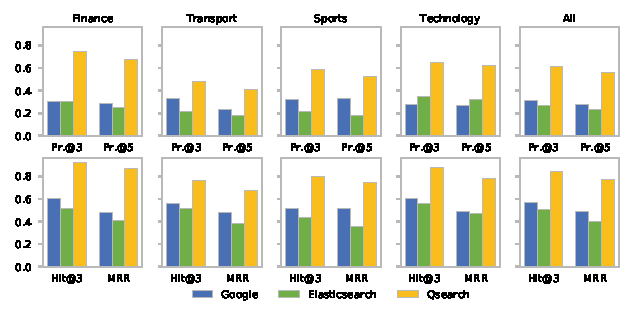
\includegraphics[width= 1\textwidth]{figures/compare.pdf}
	\caption{Comparison of Qsearch against baselines.}
	\label{fig:top-3_comparison}
\end{figure}

Overall, Qsearch performs amazingly well, typically with MRR around 0.7 or better.
The best results are for the 
Finance domain, which has the highest share in the corpus and is most represented in the
Qfact extraction training.
%Finance is the dominating slice of news articles and it covers two most frequent sample categories, Money and %Percentage, in our training dataset. 
%We can also observe that \textit{Precision@k} decreases sharply as \textit{k} increases, together with a high %\textit{MRR} and \textit{Hit} values for our both ranking models, which confirms that relevant entities are ranked higher %by our system than the irrelevant ones. 
\textit{Precision@1} is pretty good, but precision drops substantially when going deeper in the rankings. 
The embedding-based ranking model clearly outperformed the KL-divergence method
by a significant margin.
 
Figure~\ref{fig:top-3_comparison} presents the comparison of Qsearch with the $ced$ ranking model 
against Elasticsearch and Google, showing the metrics \textit{Prec.@3}, \textit{Prec.@5}, \textit{Hit@3} and \textit{MRR}. The results 
clearly indicate that Qsearch outperforms both baselines by a large margin.













%!TEX root = ../main.tex

\section{Related Work}
\label{sec:related-work}

%%%GW: keep this concise
%%% if we discuss QA at length, it suggests that these prior works are highly relevant and we should have compared to them

\subsubsection{Question Answering.} 
%Many advanced factoid-based Question Answering (QA) systems have been developed, covering the both major paradigms in QA, IR-based QA on text corpora \cite{DBLP:conf/acl/WangN15, DBLP:conf/emnlp/YangYM15} and knowledge-based QA\cite{ DBLP:conf/coling/BaoDYZZ16, DBLP:conf/ecctd/Sanchez-Azqueta17}, or fusing them both \cite{DBLP:conf/acl/DasZRM17,DBLP:conf/emnlp/SunDZMSC18}, in order to handle complex compositional queries in natural language. Diverging from traditional open-domain QA, many recently developed QA systems\cite{DBLP:journals/corr/WestonBCM15,DBLP:conf/acl/RajpurkarJL18} address the reading comprehension task that requires understanding and reasoning of natural language.  However, none of these QA systems can efficiently handle processing and reasoning of quantitative information. A few state-of-the-art works\cite{DBLP:conf/cikm/JiaARSW18} focus explicitly the reasoning of temporal constraints in questions, and most of the previous works can support mainly the counting-based numeric queries. In this work, we aim to generalize the processing of quantitative information over varied numerical constraints exploiting deep semantic role labeling. Limited number of numeric relations in the Knowledge is an important bottle neck for processing quantities, and recently has been addressed in\cite{DBLP:conf/aaai/MadaanMMRS16}. Unlike our quantity-specific context extraction model, the authors presented NumberTron which aims to extract triplets for specific numeric relations from textual corpora. Tapping into semi-structured resources from Web, QEWT\cite{DBLP:conf/kdd/SarawagiC14} harnesses ambiguous and imprecise numbers in web tables and improve the performance of quantity-seeking queries.   
%KP: discussion about WikiTableQuestions ?
QA over knowledge graphs and other linked data sources has received great attention over the
last years; see \cite{DBLP:conf/rweb/UngerFC14,DBLP:journals/kais/DiefenbachLSM18} for surveys.
State-of-the-art methods 
(e.g., \cite{DBLP:conf/acl/YihCHG15,DBLP:conf/cikm/BastH15,DBLP:conf/acl/XuRFHZ16,DBLP:conf/www/AbujabalRYW18,DBLP:journals/pvldb/ZhengYZC18}) 
translate questions into
SPARQL queries, bridging the gap between
question vocabulary and the terminology
of the underlying data by means of
templates and/or learning from
training collections of question-answer pairs.
Benchmarks like the long-standing 
QALD series and other competitions
have shown great advances along these lines
\cite{DBLP:journals/semweb/UsbeckRHCHNDU19}.
However, these benchmark tasks hardly
contain any quantity queries of the kind
addressed here (even in QALD-6-task-3, only 6 out of 150 questions are of this kind, others are mostly about quantity lookup). Note that look-ups of 
quantity attributes of qualifying entities
(e.g., Jeff Bezos's net worth, 10 richest people, or fastest sprinter over 100m)
are of a different nature, as they do not
contain quantity comparisons between query
and data (e.g., worth more than 50 million USD,
running faster than 9.9 seconds).
Moreover, the scope and diversity of the benchmark queries is necessarily restricted to relatively
few numeric properties, as knowledge graphs
hardly capture quantities in their full extent (with value and unit properly
separated and normalized). This is our motivation to tap
into text sources with more extensive coverage.

QA over text has considered a wide range
of question types (e.g., \cite{DBLP:conf/emnlp/Yang0ZBCSM18,DBLP:conf/acl/GardnerC18,DBLP:conf/acl/ChenFWB17}), but there
is again hardly any awareness of quantity queries.
Keyword search, including
telegraphic queries, with quantity conditions
have been considered by 
\cite{DBLP:conf/emnlp/JoshiSC14}, and have been applied
to web tables \cite{DBLP:journals/pvldb/PimplikarS12,DBLP:conf/kdd/SarawagiC14}. 
%The approaches pursued in that context
%cannot be carried over to our setting
%where the data input is arbitrary natural language text.

\cite{DBLP:conf/sigir/BanerjeeCR09} and
its follow-up work \cite{DBLP:conf/kdd/SarawagiC14}
focused on
a specific kind of quantity query, namely,
retrieving and aggregating numerical values
associated with an attribute of a given entity
(e.g., Bezos's net worth or GDP of India). To this end, 
learning-to-rank techniques over value distributions
were developed to
counter the uncertainty in the retrieved values,
where web pages often contain crude estimates
and lack exact values.
In contrast to our setting, that work did not
consider quantities in search conditions. 
%and did not
%require inferring units and entities to which
%quantities refer.



\subsubsection{Information Extraction.}
Recognizing and extracting numeric expressions
from text has been addressed using
techniques like CRFs and LSTMs 
(e.g., \cite{DBLP:conf/aaai/MadaanMMRS16,DBLP:conf/acl/SahaPM17,DBLP:conf/sigir/AlonsoS18}).
However, this alone does not turn numbers
into interpretable quantities, with units
and proper reference to the entity with
that quantity. Only few works attempted
to canonicalize quantities by mappings
to hand-crafted knowledge bases 
of measures \cite{DBLP:conf/cikm/IbrahimRW16}, but these efforts are
very limited in scope.
The special case of temporal expressions
has received substantial attention
(e.g., \cite{DBLP:series/synthesis/2016Strotgen}), but this solely covers dates
as measures.

Most related to our approach are the works
of \cite{DBLP:conf/kdd/SarawagiC14} and \cite{DBLP:journals/tacl/RoyVR15}.
The former used probabilistic context-free grammars
to infer units of quantities, but focused specifically
on web tables as inputs.
The latter extended semantic role labeling (see below)
to extract quantities and their units from
natural language sentences.
Neither of these can be readily applied
to extracting quantities and their reference entities
from arbitrary textual inputs.
\subsubsection{Semantic Role Labeling.} Semantic role labeling (SRL) has been intensively researched
as a building block for many 
NLP tasks \cite{DBLP:journals/coling/GildeaJ02}.
%Question Answering frameworks \cite{DBLP:conf/emnlp/ShenL07, DBLP:journals/coling/SurdeanuCZ11}, as well as, in other NLP tasks, such as Information Extraction \cite{DBLP:conf/kcap/ChristensenMSE11, DBLP:conf/naacl/StanovskyMZD18}, Machine translations \cite{DBLP:conf/coling/LiuG10}, in order to exploit the semantic representation of the predicate-argument structure of a sentence in a language. 
Given a verb phrase of a sentence
viewed as a central predicate, 
%the SRL task is to assign different pre-defined roles of the verb in the sentence. 
SRL identifies phrases that are assigned to
pre-defined roles to form a frame-like
predicate-arguments structure.
%Generally, SRL \cite{DBLP:journals/coling/GildeaJ02, DBLP:conf/conll/KoomenPRY05} is considered as a classification task based on syntactic features of sentences and often uses labeled corpus, such as PropBank \cite{DBLP:journals/coling/PalmerKG05}, FrameNet \cite{DBLP:journals/lre/Baker12}. 
%
%Instead of relying on fine-tuned syntactic features of sentences, many recent literature consider word embeddings as one of the key features to learn SRL model using different  neural network methods \cite{DBLP:conf/acl/ZhouX15, DBLP:conf/acl/HeLLZ17a, DBLP:conf/emnlp/FitzGeraldTG015}. 
Modern SRL methods make use of pre-computed
word embeddings and employ deep neural networks
for role filling (e.g., \cite{DBLP:conf/acl/ZhouX15, DBLP:conf/acl/HeLLZ17a, DBLP:conf/emnlp/FitzGeraldTG015}).
%
%Task1 of this work addresses conceptually similar to the SRL task. However, we map a sentence to a general semantic representation based on different quantity-specific roles for a given numeric value from the sentence. Hence, the characteristics of these roles differ from the predicate-argument roles where verbs are technically considered as predicates. In order to learn our quantity-specific SRL model, we employ word-embedding based deep SRL model \cite{DBLP:conf/acl/HeLLZ17a}.
Our approach differs from this state-of-the-art SRL,
as we are not primarily focused on the verb-phrase
predicate, but consider the numeric quantity in a sentence
as the pivot and aim to capture quantity-specific roles.

%%%GW: need to trim the following
To support exploration of quantitative facts in financial reports, \cite{Lamm2018QSRLA} proposed a 
semantic representation for quantity-specific roles.
% and discuss possibilities to utilize the shallow semantic parsing to develop their proposed framework. 
%In the similar direction, in order to solve the elementary school math problems, 
\cite{DBLP:journals/tacl/RoyVR15} devised a quantity representation as an additional component of
an SRL method, which is part of the Illinois Curator software suite.
% to reason about numbers in natural language. 
%
%Our SRL model represents a simplified version of their proposed semantic roles. For example, the roles \textit{entity}, \textit{value}, \textit{unit}, and \textit{resolution} are respectively similar to the roles  \textit{THEME}, \textit{VALUE with SIGN}, \textit{UNIT}, and \textit{MANNER} in their model. However, the  \textit{context} in our model generalizes the roles  \textit{QUANTITY}, \textit{LOCATION}, and \textit{TIME} together from QSRL model by Lamm et al. \cite{Lamm2018QSRLA}. Such generalization of semantic role makes our model simpler and helps in leveraging the problem of numerical Question Answering, addressed in this work. 
Our approach makes use of this technique,
%which is part of the Illinois Curator software suite,
as a preprocessing step.
However, we go further by 
learning how to connect quantities with their
respective entities and to collect relevant 
context cues that enable our matching and
ranking stage for query answering.




%!TEX root = ../main.tex

\section{Conclusion}
%We presented a method for learning rules that may contain negated atoms from KGs that
%dynamically exploits feedback from a precomputed embedding model. 
%Our approach is general in that any embedding model can be utilized including text-enhanced ones, which indirectly allows us to 
%harness
%unstructured 
%web sources 
%for rule learning.
% We evaluated our approach with various configurations on real-world datasets and observed significant improvements
%over state-of-the-art rule learning systems.\looseness=-1
%
%An interesting future direction is to extend our work to more complex non-monotonic rules with higher-arity predicates,
%aggregates and existential variables or disjunctions in rule heads, which is challenging due to inevitable scalability issues.

Awareness of entities and types has greatly advanced semantic search
both for querying the web of linked data and for Internet search engines.
In contrast, coping with quantities in text content and in query constraints
has hardly received any attention, yet is an important case.
This paper has presented the Qsearch system for full-fledged support of
quantity queries, through new ways of information extraction and 
answer matching and ranking.
We capture quantities in their full extent, including units of measures,
reference entities and the relevant contexts.
The model for Qfacts and Qqueries is relatively simple but highly versatile and effective.
%a more detailed structured modeling would not be able to cope with the
%uncertainty in textual inputs and the approximate matching of candidate answers.
A key asset of Qsearch is its high quality in extracting Qfacts,
recognizing the right entity-quantity pairs even in complex sentences.

Future work includes devising additional ways of aggregating Qfacts with
the same candidate answer, so as to obtain strong signals from many
noisy cues (i.e., when the same entity-quantity pair occurs in many pages,
but mostly in the form of crude estimates or vague hints).
Also, we plan to extend the Qquery model to incorporate queries that
contain multiple quantity conditions (e.g., hybrid SUVs with range above 500 miles
and energy consumption above 40 MPGe).








%\paragraph*{Acknowledgements.}

%\documentclass[a4paper]{llncs}

%\documentclass{llncs}
%
\usepackage[T1]{fontenc}
\usepackage{lmodern}
\usepackage[utf8]{inputenc}
\usepackage{amsfonts}
\usepackage{eurosym}
\usepackage{amsmath}
\usepackage{amssymb}
\usepackage{booktabs}
\usepackage{makeidx}  % allows for indexgeneration
\usepackage{epsfig} 
\usepackage{cite}
\usepackage{color}
\usepackage{multirow}
\usepackage{mathtools}
\usepackage{subfig}
\usepackage{hyperref}
\usepackage[para]{footmisc}
\hypersetup{
    colorlinks=true,
    %linkcolor=blue,
%    filecolor=magenta,      
    urlcolor=blue,
    citecolor=blue,
    linkcolor=blue,
}

\usepackage[inline]{enumitem}


\usepackage{llncs-space}

\newcommand{\G}{\ensuremath{\mathcal{G}}\xspace}
\newcommand{\X}{\ensuremath{\mathcal{X}}\xspace}
\newcommand{\C}{\ensuremath{\mathcal{C}}\xspace}
\newcommand{\R}{\ensuremath{\mathcal{R}}\xspace}
\newcommand{\PG}{\ensuremath{\mathcal{P}}\xspace}
\newcommand{\PW}{\ensuremath{\mathsf{PW}}\xspace}
\newcommand{\sem}[1]{[|#1|]}
\newcommand{\set}[1]{\{#1\}}
\newcommand{\incl}{\subseteq}
\renewcommand{\L}{\ensuremath{\mathcal{L}}\xspace}

\newtheorem{task}{Task}


%%% \squishlist definition, list with reduced margins
\newcommand{\squishlist}{
 \begin{list}{$\bullet$}
  { \setlength{\itemsep}{0pt}
     \setlength{\parsep}{3pt}
     \setlength{\topsep}{3pt}
     \setlength{\partopsep}{0pt}


     \setlength{\leftmargin}{1em}
     \setlength{\labelwidth}{1em}
     \setlength{\labelsep}{0.5em} } }

\newcommand{\squishlisttwo}{
 \begin{list}{$\bullet$}
  { \setlength{\itemsep}{0pt}
    \setlength{\parsep}{0pt}
    \setlength{	opsep}{0pt}
    \setlength{\partopsep}{0pt}
    \setlength{\leftmargin}{2em}
    \setlength{\labelwidth}{1.5em}
    \setlength{\labelsep}{0.5em} } }

\newcommand{\squishend}{
  \end{list}  }
%\renewcommand{\baselinestretch}{0.99}

\begin{document}
%
\frontmatter          
%



\pagestyle{headings}  

\mainmatter               
%
\title{Qsearch: Answering Quantity Queries from Text}

\author{%
Vinh Thinh Ho$^{1}$,\ \ 
Yusra Ibrahim$^{1}$,\ \ 
Koninika Pal$^{1}$,\\
Klaus Berberich$^{1,2}$,\ \ 
and Gerhard Weikum$^{1}$
}		
\institute{
$^1\ $Max Planck Institute for Informatics, Saarbr\"ucken, Germany\\
$^2\ $Saarland University of Applied Sciences, Saarbr\"ucken, Germany
}


\maketitle        

\begin{abstract}
%%%Motivation and Problem
Quantities appear in search queries in numerous forms: 
%to find a products within a specific price range, 
%to locate a country with an increasing GDP, to identify athletes who won multiple Olympic medals, among others.
companies with annual revenue of at least 50 Mio USD,
athletes who ran 200 meters faster than 19.5 s, 
electric cars with range above 400 miles, and so on.
Processing such queries requires the understanding of numbers present in the query to capture the contextual information about the queried entities. 
Modern search engines and QA systems
%like Google, Bing, etc. 
can 
%efficiently 
handle queries
that involve entities and types, 
%which need to exploit only relational structures embedded in Web content and social media for queried entities. 
%But they fail to produce crisp answers to the queries involving numerical constraints as they disregard the reasoning %over quantitative information.
but they often fail on properly interpreting quantities in queries and candidate answers
when the specifics of the search condition (less than, above, etc.), the units of interest (seconds, miles, meters, etc.)
and the context of the quantity matter (annual or quarterly revenue, etc.).
%  
%Numeric answers for such queries might appear in various sources, either structured (e.g. tables, lists), or unstructured (e.g. text), where processing unstructured text are more challenging. 
%Modern search engines like Google, Bing, etc. support queries that involve relational structures embedded in Web content and social media and can provide crisp answers to the queries or questions. However, informative quantities are usually disregarded. 
%
%Approach and  Contribution
In this paper, we present a search and QA system, called Qsearch, 
that  
%tackles queries with numerical constraints by harnessing quantitative  contextual information about entities from text.
can effectively answer advanced queries with quantity conditions.
%In particular, we propose a framework for representing quantitative information, 
Our solution is based on a deep neural network for extracting quantity-centric tuples from text sources,
%an efficient deep neural network for extracting these information from textual data, 
and a novel matching model to 
%produce 
retrieve and rank
answers 
%for given numerical queries. 
from news articles and other web pages.
Experiments 
%on real-world data 
demonstrate the effectiveness of Qsearch on benchmark queries collected by crowdsourcing.

\end{abstract}

\begin{keywords}
Semantic Search, Question Answering, Information Extraction, 
%Numeric 
Quantities
\end{keywords}

%!TEX root = ../main.tex

\section{Introduction}\label{sec:intro}

\subsubsection{Motivation.}


Quantities, such as \$2B, 40 mpg or 19.19 s,
are more than mere numbers; they express measures 
like revenue, fuel consumption or time in a race
with a numeric value and a corresponding unit. 
The occurrence of a quantity in the text or a table of a web page is associated 
with an entity and interpretable only with the surrounding context. 
%The interpretation of these quantities is only possible through the associated entities and in context. 
For example, in the sentence \textit{``BMW i8 costs about 138k Euros
in Germany and has a battery range between 50 and 60 km.''},
the quantity \euro 138.000 (after normalization) refers to the price
of the car model BMW i8, and the quantity interval [50,60]km
denotes the range for that car (note that this is in electric mode only as this is a hybrid car).

Quantities are common in search queries, for example to find a product within a specific price range,  cars or mobile phones with
desired technical or environmental properties,
or athletes who ran a race in a certain time. 
 When a user issues a quantity search query, such as \textit{``Hybrid cars with price under 35,000 Euros and battery range above 100 km''}, 
 she expects the search engine to understand the quantities and to return relevant answers as a list of entities.
%The relevant answer here is a list of cars that are ``less than 35,000 Euros'' and ``battery range more than 100km''. 
However, Internet search engines treat quantities largely as strings ignoring their values and unit of measurements. As a result, they
cannot handle numeric comparisons, they miss out on units
or scale factors (such as ``k'' in ``138k''), do not know about
necessary conversions between units,  and ultimately
fail. The exceptional cases where search engines 
(incl. vertical product search) provide 
support for coping with quantities are money and date,
but this is achieved by specialized techniques and 
fairly limited. 

\input{tables/kg_stats}

One would hope that semantic search over knowledge
graphs (KG) like DBpedia
%, Yago
 or Wikidata goes further,
%but they provide a very low coverage of quantitative facts; 
but their coverage of quantitative facts is very limited
and most literals, apart from dates, are merely represented as strings; e.g., battery capacity of the BMW i3 is shown as the string
\textit{``i3 94 A·h: 33 kWh lithium-ion battery''} in DBpedia.
%display size for mobile phones are represented by number without any associated unit in DBpedia. 
%%The length of the Mercedes-Benz O405 is shown as \textit{``11.1 m''} 
%The weight of the racing car Williams FW07 is shown as \textit{``: 585 kg''} 
%%in DBpedia 
%-- again just a string that is useless for queries with comparisons 
%like vehicles with \textit{``length more than 10 meters''} or \textit{``length above 30 feets''}.
%like cars with \textit{``weight more than 500 kilograms''} or \textit{``weight above 1000 pounds''}.
Important properties for cars, like fuel consumption, CO2 emission, etc. are not covered at all.
%in either DBpedia or Wikidata.
%though these informations are mentioned in additional comments in form of text. 
 Table \ref{table:kg_stats} gives exemplary numbers for the quantity coverage in Wikidata and DBpedia.
%show such low coverage of quantitative facts available in these KGs.
%For some cars like Tesla Model X, the range is shown in the form ``257$\pm$1 mile'' in Wikidata-- again just a string, while API returns simply a point value, 257 mile, rather providing the range that is useless for queries with comparisons 
%the length of the BMW i8 is shown as ``4,689 millimeter'' in Wikidata;
%like ``range above 250 miles''
%or ``range above 400 km''.
% For example, the range of the Tesla Model X is shown as ``257$\pm$1 mile'' in Wikidata -- just a string that is useless for queries with comparisons like ``range above 250 miles'' or ``range above 400 km''; fuel consumption, CO2 emission, etc. are not covered at all.

%Moreover, question answering systems over linked data (incl. KGs)
%have rarely considered quantities in search condition, e.g., a popular benchmark for quantity queries, QALD-6-task-3~\cite{DBLP:journals/semweb/UsbeckRHCHNDU19}, contains only 6 queries with quantity conditions out of 150.

%While range, display size and personal best time are important properties for entity types car, mobile and marathon runner, respectively; these data are not available at all, or the data type is not always included. The exception is stadium capacity, but the number in this case is dimensionless, which is easier to handle.

%Several form-based search engines were created to counter this issue, such as specialized products search engines. However, these form-based search engines are tedious to use and only covers a specific class of items, normally stored in a single relational database. 

%It is complex to find the central entitiy, and 
%uantities appear in search queries in numerous forms: to find a product within a specific price range, to locate a country with an increasing GDP, to explore movies produced in a specific year, to identify athletes who won multiple Olympic medals, among others. They represent an indispensable part of the query that defines the set of the possible answers. Therefore, they necessitate special handling to understand them within their context.

%the current gap in the search engines
 %Natural language queries involving quantities are common. However, modern search engines fail to answer them. Most of the search engines are keyword-based or entity-based.

 %As a result, they treat quantities as a string ignoring their values and unit of measurements.  Moreover, search engines usually retrieve a ranked list of webpages, except for some cases at which search queries involves prominent entities or events.   

%%%GW: now make a crisp statement of what this paper is about
This paper sets out to provide support for answering quantity queries from text, over a wide variety of expressive measures, to overcome
this severe limitation of today's search engines and knowledge graphs.
%GW: added a sentence towards "semantic web"
Our method extracts quantity-centric structure from Web contents, uncovering the hidden semantics
of linking quantities with entities. 

%% what we aim at
%To bridge this gap, we aim at answering quantity queries and providing the user with a seamless search experience.
%We define a quantity query as a query for a specific type of entities, such as cars, that is conditioned on a quantity, such as ``price less than 35,000 Euros''.

%We provide the user with a ranked list of entities, instead of a ranked list of web pages. We pay special attention to quantities in the query and their context while retrieving the answer. Thus, we provide the basis for the next generation search engine capable of answering complex quantity queries. 


 
\subsubsection{Problem Statement.}
We define our problem as follows. Given a quantity query and a corpus of text pages, 
find a ranked list of entities that match the given query.
A quantity query is a triple $(t^*,q^*, X^*)$, where 
$t^*$ is the semantic type of the expected answers, 
$q^*$ is a quantity-centric search condition, and 
$X^*$ is the context that connects the entity type  $t^*$ with quantity condition $q^*$. For example, for the query  \textit{``Cars with price less than \euro 35,000 in Germany''}, the triple $(t^*,q^*, X^*)$ is: $(\textit{cars; < \euro 35.000;} \{\textit{price, Germany}\})$.
%
Our problem has two dimensions.
The first is to understand the content of the text snippets and extract the relevant quantity facts. The second is to match such extracted
assertions (inevitably with noise and errors) against a query
and compute a ranked list of relevant entity answers.


\subsubsection{Approach.}
This paper presents Qsearch, an end-to-end system for answering quantity queries. Qsearch employs a deep neural network
to extract quantity facts from text,
%GW: added a pitch on "semantics"
this way lifting textual information into semantic structures.
%and to understand the users' quantity query. 
Then, it utilizes 
a statistical matching model to retrieve and rank answers.
%On the other hand, we preprocess the corpus of web documents into triples of $(E,Q,X)$, where $E$ is an entity, $Q$ is a quantity related to $E$, and $X$ is the context defining the relation between $E$ and $Q$. For example, the triple \textit{(BMW i8, \{costs, Germany\}, \euro 138.000)} corresponds to the following sentence: \textit{``The BMW i8 costs about \euro 138k in Germany.''}
 %Then, we semantically match the query to the facts we extract from the web corpus. We generate a ranked list of objects matching the query.
%challanges 
%how we do it
%We split the quantity search problem into two essential components: 
%(i)\emph{Quantity-fact extraction from text} (ii)\emph{Query matching}

We model the first component, quantity fact extraction, as a Semantic Role Labeling (SRL) task \cite{DBLP:journals/coling/GildeaJ02} and devise a 
%{Deep Semantic Role Labeling (DSRL)} 
deep learning
method to label words in the sentences with relevant roles. We label each word as entity, quantity or context (or other). Then we use these tags to extract quantity fact triples in form of \textit{(entity, quantity, context)}.
%
For the second component, query matching, we devise a 
%deep 
novel
%semantic
matching method to retrieve a ranked list of relevant entities that answer the user's quantity query.
%more about the approach here!

%We design a full-fledged system that answers complex quantity queries. preprocesses web content, index them, and answers complex quantity queries in an efficient manner.  Our system extracts quantity-related facts from web pages and stores them as a triple of  $(E, Q, X)$. It transforms the problem to a \emph{Semantic Role Labelling} task and employs a \emph{Deep Semantic Role Labeling (DSRL)} model to label sentences. % with $E$, $Q$, and $X$ tags.

%\subsubsection{Limitations of Prior Work.}
%\subsubsection{Outlook}
% research focused on answering quantity queries 
%recent work covering quantity extraction and fact extraction
%QA

%%%GW: this is too long for here (intro)
%Though, some of the previous work tackled, binary and n-ary quantity fact extraction~\cite{DBLP:conf/www/ErnstSW18} and semantic annotation of quantities\cite{DBLP:conf/cikm/IbrahimRW16, Ibrahim:ICDE2019}, none of them looked into how to harness these semantic annotations to answer quantity-related queries. 
%Zhang et al.~\cite{DBLP:conf/sigmod/ZhangC13} consider semantic matching of quantities on web tables, but did not give attention to quantities in natural text.  The work of Banerjee et al.~\cite{DBLP:conf/sigir/BanerjeeCR09} answers quantity consensus queries, however, they only consider binary relations and rely on hand-crafted rules. 
%State of the art retrieval models do not focus on quantity queries nor do they consider extracting quantity facts from the text. On the other hand factoid question answering (QA) systems merely function as a quantity-lookup form structured semantic knowledge. Other QA systems have been proposed to answer reading comprehension questions, however, they do not aggregate answers from multiple sources and they focus on general questions rather than quantity queries. 


%On the other hand, we employ \emph{Deep Semantic Role Labeling  (DSRL)} to extract n-ary quantity facts, and provide a robust system to process and answer quantity queries.

\subsubsection{Contribution.}
The salient contributions of this work are as follows:
\begin{itemize}
\item We present Qsearch, a system for answering quantity queries from text.
\item We propose a deep neural network for quantity fact extraction, and a matching model for answering quantity queries.
\item  We present extensive experiments on benchmark queries collected by crowdsourcing.%, demonstrating the effectiveness of our approach with respect to the correctness of answers.

%\item We make code, data and a running demo available to the research community at\\{\small\url{http://anonymous-for-double-blind-review/}}.
\end{itemize}

\section{Computational Model and System Overview}
In this section, we introduce the computational model for our
approach and give an overview of the Qsearch system and its components.

\subsection{Model for Facts, Queries and Answers}
\label{sec:framework}

%In this paper we present two models, the first is the \texttt{Quantity Fact Extraction} model and the second is the \texttt{Matching} model.
%We formalize the notions of quantity facts, quantity queries
%and answers to queries as follows. 

%In this section, we start by introducing some definitions to lay the foundation for our model. Then, we present our model and specify its inputs and outputs.

%In this section, we introduce our computational model for answering numerical queries, that would be exploited to develop our methodology to extract answers from text later on. In particular, we compose the following definitions:


%This numerical fact representation is quite close to the traditional RDF representation \cite{rdf},  which models each fact as a \textit{(subject, predicate, object)} triple. While the  entity $E$ and quantity $Q$ play as the \textit{subject} and \textit{object} in the RDF model respectively, the context $X$ works like a \textit{predicate}. However, instead of using a unique predicate for all the facts with the same predicate meaning as in the RDF model, we represent $X$ as a set consisting of tokens that could explain the connection between $E$ and $Q$. That is, in a sentence $S$ containing some entity $E$ and quantity $Q$, the context $X$ is determined as a subset of important words from $S$ which could clarify the role of $Q$ with regard to $E$. 


%%%%%%%%%%%%%%%%%%%%%%%%%%%%%%%%% QFE %%%%%%%%%%%%%%%%%%%%%%%
%\subsubsection{Quantity Fact Extraction Model}
\subsubsection{Extraction Model.}
%start from here 
The \textit{input} of this model is a corpus of text documents $\mathcal{T}$ with text snippets (e.g., sentences or paragraphs) that contain
%$n$ 
entity and 
%$m$ 
quantity mentions. 

The \textit{output} of this model is a set of \textit{quantity facts} extracted from the text corpus, $\mathbb{F} =\{\mathcal{F}_1, \mathcal{F}_2, ...\}$, where a quantity fact is defined as follows.


\begin{definition}[Quantity fact] A quantity fact (Qfact) is a triple $\mathcal{F} = (e,q,X)$, where: \\
- $e$ is an entity;\\
- $q = (v,u,r)$ is a quantity consisting of a numerical value $v$, a canonicalized unit $u$ (e.g., km, \$) and a value resolution $r$ (exact, approximate, upper/lower bound, %range
interval);\\
- $X = \{x_1,x_2,...\}$ is a context, which is a bag of words describing the relation between $e$ and $q$.
\end{definition}


\begin{example}
Given the text snippet \textit{``BMW i8 costs about 138k Euros in Germany and has a battery range between 50 and 60 km.''}, we can extract the following Qfacts:\\
- $\mathcal{F}_1: e=\textit{BMW i8}; q=\textit{(138.000, \euro, approximate)}; X = \{\textit{costs, Germany}\}$\\
- $\mathcal{F}_2: e=\textit{BMW i8}; q=\textit{(50-60, km, interval)}; X = \{\textit{range, battery}\}$ 
\qed 
\end{example}


The Qfact representation is similar to the RDF model
\cite{rdf}, 
which
represents each fact as a \textit{(subject, predicate, object)} triple.  In  the Qfact model,  the  entity $e$ and the quantity $q$  correspond to the \textit{subject} and the \textit{object}, respectively. 
The context $X$ in Qfacts is a proxy for the \textit{predicate} in the RDF model. However, it differs in two essential points: first, the context $X$ can capture more than one relation between $e$ and $q$; second, the context $X$ consists of a set of non-canonicalized tokens, instead of a unique canonicalized predicate in a knowledge graph. 

This relaxed representation is a judicious design choice and
essential for the flexibility of our approach: first, we can represent complex n-ary facts using a simple Qfact triple; second, our model can generalize to unseen relations; third, our model can cope with the 
inevitable diversity
and uncertainty in the language expressions of the underlying
text snippets. 
In theory, it is conceivable that all arguments that appear in
the context $X$ are also individually extracted and canonicalized
 to fill the slots of a frame-like structured record.
However, approaches along these lines do not work robustly and
suffer from heavy propagation of noise and errors.


The Qfact model allows different representations of the same fact,
and the underlying text corpus may express the same 
knowledge by different paraphrases. Hence, 
Qfacts are more expressive towards answering queries
via approximate matches and related phrases.
%provides a flexible model to represent the various information expressed in the text.

%%%%%%%%%%%%%%%%%%%%%%%%%%%%%%%%%%%%%%%%%%%%%%%%%%%%%%

%%%%%%%%%%%%%%%%%%%%%%Matching
\subsubsection{Matching Model.}

The \textit{input} of this model is a set of Qfacts $\mathbb{F} =\{\mathcal{F}_1, \mathcal{F}_2, ...\}$
extracted from the text corpus, and  a \textit{quantity query} $\mathcal{Y}$ defined as:


\begin{definition}[Quantity query] A quantity query (Qquery) is a triple $\mathcal{Y} = (t^*,q^*,X^*)$ where: \\
- $t^*$ is the semantic type of the target answers;\\
- $q^* = (v,u,o)$ is a quantity condition consisting of a numerical value $v$, a canonicalized unit $u$ 
(e.g., km, \$)
, and a comparison operator $o$ (exact, approximate, upper/lower bound, 
%range
interval);\\
- $X^* = \{x_1,x_2,...\}$ is a context condition, 
expressed by a bag of words that describes the 
relation between $t^*$ and $q^*$.
\end{definition}

\begin{example}
\label{ex:qquery}
Given the query \textit{``Cars with price less than 100k Euros in Germany''}, its corresponding Qquery is  as follows:\\
- $\mathcal{Y} : t^* = \textit{car}; q^*=\textit{(100.000, \euro, upper bound)}; X^* = \{\textit{price, Germany}\}  $
\qed 
\end{example}

%The definition of the Qquery is analogous to that of the Qfact. Such that, 
Each part of a Qquery imposes a constraint on its 
counterpart in a Qfact considered as a candidate answer.

\begin{definition}[Query answer] 
 A Qfact $ \mathcal{F} =(e,q,X)$ is an answer for a Qquery $\mathcal{Y} = (t^*,q^*,X^*)$ iff 
(1) $e$ is an entity of type $t^*$, 
(2) the quantity $q$ satisfies the quantity condition $q^*$ and (3) the context $X$ (approximately) matches the context condition $X^*$.
\end{definition}

\begin{example}
Consider the Qquery in Example \ref{ex:qquery} and the two text segments
 \textit{``German dealers sell the BMW X3
 at a price as low as 55,000 Euros''} and
 \textit{``Car dealers in Munich sell the BMW X3
starting at 55,000 Euros''}.
The Qfact extracted from the first snippet
with 
$e=\textit{BMW X3},
q=\textit{(55.000, \euro, lower bound)}$,
and $X = \{\textit{German, dealers, sell, price}\}$
is a strong match for the query;
whereas the Qfact extracted from the second snippet
with 
$e = \textit{BMW X3},
q=\textit{(55.000, \euro, lower bound)}$,
and $X = \{\textit{car, dealers, Munich, sell}\}$
is an approximate match (by embedding-based relatedness).
\qed 
\end{example}

The \textit{output} of this model is a ranked list of entities $\mathcal{E}^* = \{e_1, e_2, e_3,...\}$ from matching Qfacts with the Qquery, which will be discussed in Section \ref{sec:match}.

%%%%%%%%%%%%%%%%%%%%%%%%

\subsection{Qsearch System}
Figure \ref{fig:system} 
%shows the high-level architecture of 
gives an overview of the architecture of 
Qsearch. The arrows in the figure depict information flow between the different system components. 
Qsearch consists of two main stages:
\textit{Extract}
and \textit{Answer}.
 
%In this section, we demonstrate our numerical question answering system from text. In Figure \ref{fig:system}, we present a high-level architecture of our system, where the arrows depict information flow between building blocks. We split the working flow of our system into two main stages: \textit{Extract} and \textit{Answer}.

\begin{figure}[t]
\centering
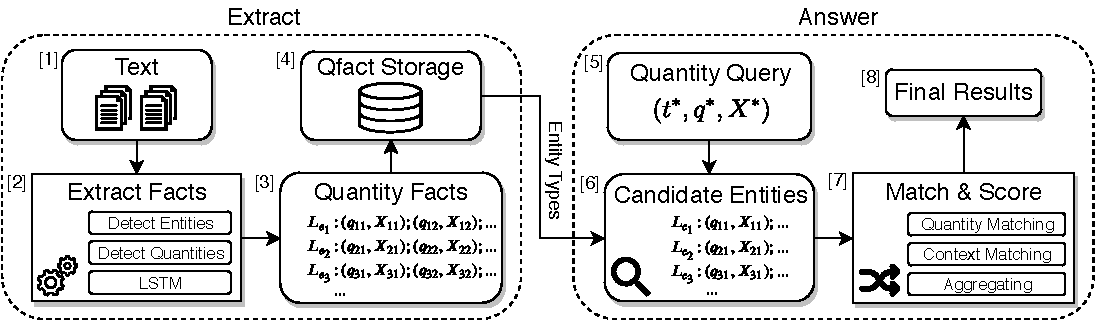
\includegraphics[width=1\textwidth]{figures/overview.pdf}
\caption{Overview of Qsearch.}
\label{fig:system}
\end{figure}
% what is the storage, how is it stored, and indexed 

\subsubsection{Extract.}  
We preprocess the text corpus (Block 1) to recognize
and disambiguate named entities 
%using the AIDA \cite{DBLP:conf/emnlp/HoffartYBFPSTTW11} system,
%which links named entities to the YAGO knowledge base\cite{DBLP:conf/www/SuchanekKW07}. 
and link them to an external knowledge base (KB). We also identify mentions of quantities in the text and normalize them into standard units. 
Subsequently, we run a deep neural network to extract Qfacts from the preprocessed text (Block 2). We learn and employ a specifically designed
Long Short Term Memory (LSTM) network, which will be described in Section \ref{sec:extract}. 

Extracted Qfacts are organized and grouped by their named entities, such that each individual entity $e_i$ is mapped to a list of quantities and related contexts $L_{e_i} = \{(q_{i1},X_{i1}),(q_{i2},X_{i2}),... \}$ (Block 3).
All extracted Qfacts are stored in a data repository (Block 4, 
based on Elasticsearch in our implementation), where entities are linked to their semantic types from the KB.
%We use AIDA \cite{DBLP:conf/emnlp/HoffartYBFPSTTW11} for entity linking, YAGO \cite{DBLP:conf/www/SuchanekKW07} for entity typing, and ElasticSearch as a storage engine.



\subsubsection{Answer.}
We answer incoming Qqueries by matching them against
the Qfacts from the \textit{Extract} stage. 
For a Qquery $(t^*,q^*,X^*)$ (Block 5), we first apply 
an entity-type filter, eliminating entities with the wrong type. 
This results in a set of candidate entities $\mathcal{C} = \{c_1,c_2,...\}$ (Block 6) satisfying the type constraint $t^*$, along with their quantity-context pairs $\{L_{c_1},L_{c_2},...\}$. 
In Block 7, we discard all candidate answers 
%with quantity-context pairs $(q,X) \in L_c$ 
that do not satisfy the quantity condition $q^*$.
Finally, we compute a matching score for each candidate entity $c \in \mathcal{C}$ based on the contexts $X$ in the
quantity-context pairs $L_c$, using a statistical language model
or a text embedding method, which will be described in Section \ref{sec:match}. The candidate entities are ranked by their scores and returned to the user (Block 8). 

In the following Sections
\ref{sec:extract} and \ref{sec:match}, we discuss in detail the
 Qfact extraction model and the matching and answering model, 
respectively.

%In the remainder of this section, we discuss how each candidate entity is scored in Block 7.

\section{Quantity Fact Extraction From Text}
\label{sec:extract}
In this section, we describe our method for extracting Qfacts from natural language text.
%which are then used to answer quantity queries. 
At the core of our solution is a deep-learning neural network for sequence tagging, running on individual sentences. 
%Moreover, we suppose that the input sentence is pre-processed by detecting entities and quantities in advance.

\subsubsection{Input Preprocessing.} In the first step, we preprocess the input text corpus by detecting entities and quantities appearing in each individual input sentence.  
We perform Named Entity Disambiguation (NED) 
using the AIDA \cite{DBLP:conf/emnlp/HoffartYBFPSTTW11} system,
which links named entities to the YAGO knowledge base\cite{DBLP:conf/www/SuchanekKW07}. To achieve a better detection quality, we run NED on a per-document instead of per-sentence basis.
For detecting quantities, we make use of the Illinois Quantifier \cite{DBLP:journals/tacl/RoyVR15}, a state-of-the-art tool for 
recognizing numeric quantities in text, along with some hand-crafted rules (e.g., regular expressions). 
Subsequently, each identified quantity is replaced by a placeholder \textit{``\_QT\_''}. 
\begin{example}
\label{ex:3}
Input and output of this preprocessing step look as follows:
{\small
\begin{align*}
\textit{sentence} &\ |\ \textit{BMW i8 has price of 138k Euros in Germany and range from 50 to 60 km on battery .} \\
\textit{preproce}&\textit{ssed}\ |\ \overbrace{\textit{BMW i8}}^{\mathclap{e_1=\textit{<KB:BMW\_i8>}}}\textit{ has price of }\underbrace{\textit{\_QT\_}}_{\mathclap{q_1=\textit{(138.000,\euro,appr.)}}}\textit{ in }\overbrace{\textit{Germany}}^{\mathclap{e_2=\textit{<KB:Germany>}}}\textit{ and range } \underbrace{\textit{\_QT\_}}_{\mathclap{q_2=\textit{(50-60,km,interval)}}}\textit{ on battery .}  \tag*{\qed}
\end{align*}
%%%GW:  Q - uppercase - is a Qfact. For quantity alone, we should use q - lowercase.
}
\end{example}
\subsubsection{Sequence Tagging Model.} In the second step, we aim to extract complete Qfacts from the preprocessed sentences. 
For each quantity detected in the previous step, we want to identify the entity to which it refers
and the relevant context tokens that express the entity-quantity relation.
\begin{example} 
Consider the preprocessed sentence in Example \ref{ex:3}. If we use the first quantity $q_1 = \textit{(138.000, \euro, approximate)}$
as the input's pivot, 
we want to obtain the output $e(q_1) = e_1 = \textit{<KB:BMW\_i8>}$ and $X(q_1)=\{\textit{price, Germany}\}$. 
Analogously, with $q_2 = \textit{(50-60, km, interval)}$ as pivot,  the desired output is 
$e(q_2)= e_1 = \textit{<KB:BMW\_i8>}$ and $X(q_2)=\{\textit{range, battery}\}$. \qed
\end{example}
We formalize this task as a sequence labeling problem as follows.
\begin{task}[Quantity Fact Extraction]
Given a preprocessed sentence $S$ with the set of detected entities $\mathcal{E} = \{e_1,e_2,...\}$, the set of detected quantities $\mathcal{Q} = \{q_1,q_2,...\}$ and a selected pivot quantity of interest $q_i \in \mathcal{Q}$, the task of quantity fact extraction is to label each token of the sentence with one of the following tags: (i) \textit{<E>}, for denoting the entity that $q_i$ refers to; (ii) \textit{<X>}, for denoting the context tokens that relate $q_i$ and its entity; and (iii) \textit{<O>}, for all other tokens.
\end{task}
\begin{figure}[t]
\centering
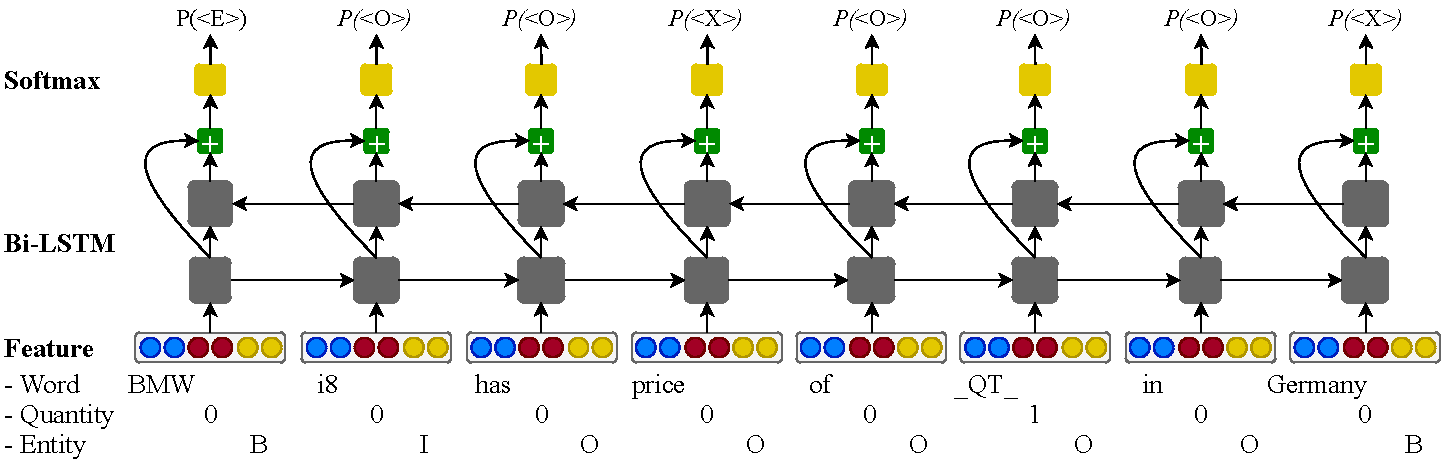
\includegraphics[width=1\textwidth]{figures/neural.pdf}
\caption{The Qfact extraction model used by Qsearch.}
\label{fig:neural}
\end{figure}
Our problem resembles the Semantic Role Labeling task \cite{DBLP:journals/coling/GildeaJ02}, which is typically addressed by
Conditional Random Fields (CRFs)
or Long Short Term Memory (LSTM) models. 
Figure \ref{fig:neural} depicts the bi-directional LSTM model 
that we devised for this task, inspired by prior work \cite{DBLP:conf/acl/HeLLZ17a}.
 Other models for sequence labeling (e.g., \cite{DBLP:conf/acl/ZhouX15, DBLP:conf/emnlp/FitzGeraldTG015})
could be easily incorporated as well. 
Our labeling network consists of three layers: Input Features, Bi-LSTM, and Softmax. 
While this general architecture is close to any other LSTM model, the most unique point here is the input representation,
as described next.

\subsubsection{Input Features.} Each token of the preprocessed input sequence is represented as the concatenation of three input feature vectors:
\begin{enumerate}[label=(\it\roman*)]
\item \textit{Word}: We include word embeddings as an input feature, which enables the neural model to 
generalize to different words having similar meanings.
In our implementation, we use Glove \cite{DBLP:conf/emnlp/PenningtonSM14} precomputed embeddings.
\item \textit{Quantity}: We provide the position of the 
pivot quantity to the model as input. 
When sentences contain multiple quantities (which is a relatively frequent case), our model operates
one quantity at a time and we re-run the model for different quantities.
%which resembles the Semantic Role Labeling task, where the verbs are passed into the input instead of the quantities.
\item \textit{Entity}: We also provide information about the recognized entities as input to the neural model. 
As entities often span multiple tokens, we employ the BIO tagging mechanism \cite{DBLP:conf/acl-vlc/RamshawM95}, where a tag \textit{B} is used for tokens at the beginning of an entity name,
\textit{I} for tokens inside the name, and \textit{O} for other tokens. 
With this representation, the output of the model only needs to tag the first token of a multi-word entity name with \textit{<E>}, 
and subsequent tokens are tagged with \textit{<O>}. Figure \ref{fig:neural} shows an example: \textit{``BMW i8''} is chosen as the entity 
connected with the pivot quantity; only the first token \textit{``BMW''} is tagged as \textit{<E>} in the output.
\end{enumerate}

\subsubsection{Output Constrained Decoding.} The output of the model are the probabilities of each token word in the input belonging to each of the three tags \textit{<E>}, \textit{<X>} and \textit{<O>}, produced by the Softmax layer. 
In neural models, usually the tag with the highest score will be assigned to each token word.
%which results in the highest probability of the whole tag sequence. 
However, this standard technique would not take into account the dependencies between output tags, and hence might give us an invalid tag sequence. To solve this issue, we impose the following two constraints on the output of the model at decoding time, and find the most probable tag sequence satisfying them: \textit{(i)} only one tag \textit{<E>} can appear in the output
(namely, for the one entity to which the pivot quantity refers);
and \textit{(ii)} that tag \textit{<E>} has to be at the start token of an entity name. 


To find the most probable tag sequence, we use Dynamic Programming to decode from left to right. Specifically, we compute subsequences of tags $\textit{Seq}_{i,j,k}$ for every $i \in \{1..n\}$ ($n$ is the sentence length)$; j \in \{\textit{<E>}, \textit{<X>}, \textit{<O>}\};$ and $k \in \{0, 1\}$. Here, $\textit{Seq}_{i,j,k}$ denotes tag subsequence with the highest probability for tokens from position $1$ to position $i$, where the tag of token at position $i$ is $j$, and the subsequence contains $k$ \textit{<E>} tags.
Note that the probability of a tag subsequence is computed as the product of the probabilities of its constituent tags. 
The final tag sequence can be derived at $i = n$.

%The final tag sequence can be derived at position $i = n$.

%We compute subsequence of tags from position 0 to i, denoted as  $\textit{Seq}_{i,j,k}$ where $i \in \{1..n\}; j \in \{\textit{<E>}, \textit{<X>}, \textit{<O>}\};$ and $k \in \{0, 1\}$. Here, $\textit{Seq}_{i,j,k}$ represents that the tag of token at position $i$ is $j$ and $k$ is interpreted as the tag subsequence with the highest probability for tokens from position $1$ to $i$.
%where the tag of token at position $i$ is $j$, and the subsequence contains $k$ \textit{<E>} tags.


\subsubsection{Distant Supervision Training.} As training data is an important factor but difficult to obtain, and manual labeling 
at scale is too 
expensive, we employ distant supervision to generate training data for the Qfact extraction model.
We use unsupervised, pattern-based Open Information Extraction (Open IE) to overlay an n-tuple structure
(with triples or higher-arity tuples) 
on the input text. 
We employ the OpenIE4 tool \cite{DBLP:conf/ijcai/Mausam16} to this end, and then use its output tuples
to generate training data. This process consists of two steps:\\

\noindent \textit{- Step 1: Capture information areas:} We define an \textit{information area} as a subset of tokens from a sentence, which presents complete information about a fact.
We run Open IE on the \textit{unprocessed} sentence to detect all possible tuples expressed by the text. 
Each of these tuples has a confidence score; to ensure the quality of the generated training samples, 
we only keep tuples having a confidence score of at least 0.9. 
Each of the selected tuples corresponds to an information area.
\begin{example} Consider the unprocessed sentence in Example \ref{ex:3}, suppose the following tuples are extracted by Open IE: (1): \textit{(BMW i8; has; price of 138k Euros; in Germany)$^{0.95}$}, (2): \textit{(BMW i8; has; range from 50 to 60 km on battery)$^{0.9}$}, (3): \textit{(BMW i8; has; price of 138k Euros)$^{0.8}$}, (4): \textit{(BMW i8; has; range from 50 to 60 km)$^{0.5}$}, and (5): \textit{(BMW i8; has; price)$^{0.1}$}. We only keep high-confidence tuples (1) and (2), which contain complete information. 
Then the following information areas are chosen for training:
{\small
\begin{align*}
\mathrlap{\underbracket{\phantom{\textit{BMW i8 has }}}_{\textit{(2)}}} \overbracket{\textit{BMW i8 has price of 138k Euros in Germany}}^{\textit{(1)}} and \underbracket{\textit{range from 50 to 60 km on battery}}_{\textit{(2)}} . \tag*{\qed}
\end{align*}
}
\end{example}
\noindent \textit{- Step 2: Transform infomation areas into training samples:} We map the information areas obtained in Step 1 with entities and quantities detected from the preprocessing phase:
{\small
\[
 \mathrlap{\underbracket{\phantom{\textit{<KB:BMW\_i8> has }}}_{\textit{(2)}}} \overbracket{\textit{<KB:BMW\_i8> has price of \_QT\_}_{(1)} \textit{in <KB:Germany>}}^{\textit{(1)}} and \underbracket{\textit{range \_QT\_}_{(2)} \textit{on battery}}_{\textit{(2)}} . \tag*{\qed}
\]
}
With this mapping, information areas yield training samples for the neural network. 
We apply conservative filters so that this self-training process minimizes spurious samples.
First, we keep only information areas that contain exactly one quantity \textit{\_QT\_}, the pivot quantity. 
Second, since English sentences tend to express quantity information in active voice, 
the entity connected to the pivot quantity should appear in the first argument (subject) of the Open IE tuple. 
For instance, information area (1) has two entities \textit{<KB:BMW\_i8>} and \textit{<KB:Germany>};
we choose the former as the one to which quantity \textit{\_QT\_$_{(1)}$} refers. 
Finally, we discard all information areas where the subject of the Open IE tuple contains more than one entity.

At this point, for each information area, we have a quantity and a unique entity to which it refers. 
The context between them is determined from the remaining tokens in the information area based on their Part-of-speech (POS) tags. 
We allow only the following POS patterns to form the context: noun (NN*), verb (VB*), adjective (JJ*), adverb (RB*), and 
foreign  word (FW, to capture out-of-vocabulary names). 
We also use pre-defined stopwords to remove uninformative tokens from the context. 
The resulting Qfact, along with the \textit{<E>,<X>,<O>} tags for its token sequence, becomes a positive training sample.
%Furthermore, to prevent the tagging model from being overly optimistic, we also take into account negative training samples, 
As negative training samples, we collect all information areas where no entity could be identified to relate with the
pivot quantity, i.e., all tokens are tagged as \textit{<O>}.


%{\tt\color{red} GW: need to say more about the actual training - size of training data, which 
%software library, batch size, epoch size, learning rate etc. !!!!!!!!!!}

 
%!TEX root = ../main.tex
\section{Candidate Fact Matching Model} 
\label{sec:match}
This section describes our method to answer Qqueries from the extracted Qfacts. To this end, each Qfact is assigned a score denoting its relevance to the given Qquery.

\subsubsection{Query Parsing.} 
%We implemented a simple parser to transform the user queries into the Qquery format. 
Input questions are mapped into Qqueries by a rule-based parser for recognizing answer type and quantity condition; all other tokens (except stopwords) are included in the query context. The parser uses a dictionary of YAGO types and a dictionary of quantity units. An alternative to this rule-based technique would be to apply the same neural extraction method to questions that we have used to extract Qfacts from text. However, the questions are easier to handle, and the rule-based parser works well. 

\begin{task}[Quantity Fact Scoring] Given Qquery $\mathcal{Y} = (t^*,q^*,X^*)$ and Qfact $\mathcal{F} = (e,q,X)$, compute a distance score $d(\mathcal{F}, \mathcal{Y})$ reflecting the relevance of $\mathcal{F}$ regarding $\mathcal{Y}$.
\end{task}
Without loss of generality, we assume that a lower score denotes a better fact.
%As mentioned in Section \ref{sec:framework}, 
$\mathcal{F}$ should be a high-ranked answer for $\mathcal{Y}$ iff the following three conditions hold:
(1) $e$ is an entity of type $t^*$, 
(2) $q$ satisfies $q^*$, and (3) $X$ is a good (approximate) match for $X^*$.

%\begin{task} [Quantity Fact Retrieval] Given a quantity query $\mathcal{Q}$ and a set of candidate quantity facts $\mathbb{F} = \{\mathcal{F}_1,\mathcal{F}_2,... \}$, return a ranked list of facts $\mathbb{F}_i \subset \mathbb{F}$
%\end{task}
\subsubsection{Entity - Type Matching.} We only consider the Qfact $\mathcal{F}$ if the entity $e$ has type $t^*$. Since the entities from text are linked to an external knowledge base, we make use of the type information from the KB to filter out unsuitable facts for $\mathcal{Y}$. %This is done in Block 6 of the Qsearch overview (Figure \ref{fig:system}).

\subsubsection{Quantity Matching.} We also discard $\mathcal{F}$ if $q$ does not satisfy $q^*$. This is the case when either (1) the units of $q$ and $q^*$ relate to different concepts (e.g. \textit{km} (length) vs. \euro (money)) and are thus incomparable; or (2) their values (after conversion to the same unit) do not match the comparison operator of $q^*$. Since quantity matching is not the focus of our paper, we apply a simple matching method as follows. First, we use hand-crafted rules for unit conversions, re-scaling if needed (e.g., for kilo, mega, etc.), and value normalization. Second, we turn the quantity value into an interval based on its resolution. For example, when the query is about approximate matches, a quantity value $v$ is smoothed into the interval $[v-\delta, v+\delta]$ with a configuration parameter $\delta$. In experiments, we set $\delta$ to 5\% of $v$. A comparison is considered a match when the two intervals overlap, and their units (after conversion and re-scaling) match.

\subsubsection{Context Matching.} If the Qfact $\mathcal{F}$ satisfies the above two constraints, we will consider the similarity between the query context $X^*$ and the fact context $X$. We propose to use the following two approaches for measuring the context relevance: a \textit{probabilistic} and an \textit{embedding-based} approach.\\

\noindent \textbf{Probabilistic Ranking Model.} We adopt the Kullback-Leibler (KL) divergence between the query context $X^*$ and the fact context $X$, which is typically used in statistical language models \cite{DBLP:journals/ftir/Zhai08}. The scoring function is defined as follows:
\begin{align*}
d(\mathcal{F}, \mathcal{Y}) = \textit{KL}(X^*, X) &= H(X^*, X) - H(X^*) \\ &\equiv H(X^*, X) 
= -\sum_{w \in \mathcal{V}} P(w|X^*)\,\log P(w|X)
\end{align*}
where $\mathcal{V}$ is the word vocabulary, $H(X^*)$ is the entropy of $X^*$; $H(X^*, X)$ is the cross entropy between $X^*$ and $X$; and $\equiv$ indicates rank equivalence
(i.e., preserving order). 
Since we are only interested in ranking fact contexts in response to a query context, we can omit $H(X^*)$. The word probability $P(w|X^*)$ for the query context is estimated using Maximum Likelihood Estimation (MLE) on an expanded version $X^*_E$ of $X^*$ as:
\[P(w|X^*) = count(w \in X^*_E)/|X^*_E|\]
To expand a query context, we resort to WordNet \cite{Miller:1995:WLD:219717.219748} and add all synonyms of the context words to it. For the fact context, we estimate the word probability $P(w|X)$ using Jelinek-Mercer smoothing 
%to avoid zero probabilities
 as:
\[P(w|X) = (1 - \lambda) \times count(w \in X)/|X| + \lambda \times P(w|B)\]
This linearly combines the MLE from the fact context $X$ with the MLE obtained from a background corpus $B$. The smoothing parameter $\lambda$ (set to $\lambda=0.1$ in our system) controls the influence of the background corpus on the probability estimate. We construct the background corpus $B$ from all sentences of the entire text corpus that contain at least one quantity (total 39M sentences in our data). \\


%Since these two estimates are very sparse, before calculating, we expand $X^*$ and $X$ using an external resource. Moreover, a smoothing method is applied to avoid zero counts.
%\thinh{Should explain more? which resource, how to expand, which smoothing method.}

\noindent \textbf{Embedding-based Ranking Model}: 
We observed on our data that the query context $X^*$ is often shorter than the fact context $X$, since sentences are often more verbose than the typically short queries. Hence, to measure the distance score of $X$ with regard to $X^*$, we can match tokens between $X^*$ and $X$ using word embedding similarity as follows:
\[d(\mathcal{F}, \mathcal{Y}) = {\bigg(\sum\limits_{u \in X^*} \min\limits_{v \in X}(dist(u,v))\bigg)}/{|X^*|}\]
where $dist(u,v) \geq 0$ is the semantic distance between two words $u$ and $v$ estimated from their pre-computed word embedding vectors \cite{DBLP:conf/emnlp/PenningtonSM14}. 
We use cosine distance in the Qsearch implementation, re-scaled for normalization to [0,1]. 
In the above equation, 
we map each word of query context $X^*$ to its closest word in the fact context $X$ in the embedding space. This scoring formula gives the same weight to every token in the query context $X^*$, which might be misleading, since they could have a different degree of importance.
%Therefore, to increase the impact of more important words and to reduce the role of less %important ones in $X^*$, 
This issue is overcome by giving higher weight to important words and lower weight
to uninformative words, using
%we use 
the following distance function:
\[d(\mathcal{F}, \mathcal{Y}) = \frac{\sum\limits_{u \in X^*} W(u)\min\limits_{v \in X}(dist(u,v))}{\sum\limits_{u \in X^*}W(u)} + 1\]
where $W(u) \geq 0$ is the importance weight of word $u$. 
There are several weighting functions that can be used for $W$ (e.g., \textit{inverse document frequency (idf)}, \textit{term strength}, etc.); we use Robertson’s \textit{idf}\cite{DBLP:journals/jd/Robertson04}. 
We call the above formula the 
\textit{directed embedding distance}, $ded(X^* \rightarrow X)$,
between query and fact contexts.

$ded(X^* \rightarrow X)$ describes how well each word in $X^*$ matches with some other word in $X$, but in many cases it fails to reflect the match between their meaning. The presence of a single word in the fact context $X$ can totally change its meaning. Consider, as a concrete example, the two contexts $X^*=\{\textit{net, worth}\}$ vs. $X = \{\textit{negative, net, worth}\}$. Hence, our idea is to penalize the relevance score with an amount proportional to the directed embedding distance between $X$ and $X^*$.
Specifically, we define the \textit{context embedding distance ($ced$)} that implements this idea:
\begin{align*}
&d(\mathcal{F}, \mathcal{Y}) = ced(X^*, X) = ded(X^* \rightarrow X) \times ded(X \rightarrow X^*)^\alpha \\
=& \Bigg( \frac{\sum\limits_{u \in X^*} W(u)\min\limits_{v \in X}(dist(u,v))}{\sum\limits_{u \in X^*}W(u)} + 1 \Bigg) \times \Bigg( \frac{\sum\limits_{u \in X} W(u)\min\limits_{v \in X^*}(dist(u,v))}{\sum\limits_{u \in X}W(u)} +1 \Bigg)^\alpha 
\end{align*}
Intuitively, our $ced$ measure is the product of two components: (1) $ded(X^* \rightarrow X)$ captures how well query context tokens match with fact context, and (2) $ded(X \rightarrow X^*)$ reflects how much additional terms in $X$ shift its meaning, and hence, should be penalized. Parameter $\alpha \in [0,+\infty)$ controls how much the penalty scaling affects the total score.

\begin{example} Consider the Qquery context $X^* = \{\textit{gross, domestic, product}\}$ and two Qfact contexts $X_1 =$ \{\textit{gross, national, product}\}, $X_2 =$  \{\textit{gross, domestic, product, capita}\}. While we are more inclined to $X_1$ than $X_2$, the directed embedding distance $ded(X^* \rightarrow X_2)$ has a slightly better score than $ded(X^* \rightarrow X_1)$, as it does not penalize the word \textit{``capita''}
(which indicates that the GDP is per capita, not the total GDP). 
In contrast, $ded(X_1 \rightarrow X^*)$ is lower than $ded(X_2 \rightarrow X^*)$ (since \textit{``national''} is close to \textit{``domestic''}), preferring $X_1$ over $X_2$ with regard to $X^*$, which results in the desired ranking based on the context embedding distance $ced$. \qed
\end{example}

\subsubsection{Entity Scoring.} The output of Qsearch is a ranked list of entities from matching Qfacts with the Qquery. 
%In Block 7 of the system overview (Figure \ref{fig:system}), we give 
We assign a score for each candidate entity 
%$c \in \mathcal{C}$ based on its quantity-context pairs $L_{c} = \{(q_{c1},X_{c1}),%(q_{c2},X_{c2}),... \}$. Note that after filtering based on the quantity condition, we only need %to consider context matching.
based on one of the above context distance models and
aggregating over the entity's quantity-context pairs as follows:
\[\textit{score}(c \in \mathcal{C}, \mathcal{Y}) = \min\limits_{(q, X) \in L_c} d(\mathcal{F}=(c,q,X), \mathcal{Y})\]
where $d(\mathcal{F}, \mathcal{Y})$ is either the Kullback-Leibler divergence $\textit{KL}(X^*, X)$ or the context embedding distance
$ced(X^*,X)$.
So when the same candidate entity appears in multiple Qfacts, we pick the best-scoring
Qfact context distance.
%Put differently, we rank candidate entities based on their best fact context, i.e., the one %achieving the lowest distance to the query context.


%!TEX root = ../main.tex

\section{Evaluation}
We run experiments on a Linux machine with 80 CPU cores, 500GB RAM, and 2 GPUs. To evaluate Qsearch, we perform an intrinsic evaluation of our {\em Qfact extraction model} and an extrinsic evaluation of the {\em end-to-end Qsearch system}.
\subsubsection{Dataset.} All experiments use a large collection of news articles, compiled from two real world datasets: the \textit{STICS} project \cite{DBLP:conf/sigir/HoffartMW14} with news from 2014 to 2018, 
and the \textit{New York Times} archive
\cite{nyt}
 %5843811 + 1765538
with news from 1986 to 2008.
In total, our corpus consists of 7.6M documents.
 
\subsection{Intrinsic Evaluation of the Quantity Fact Extraction Model}
%We conduct intrinsic evaluation to examine the quality of our Qfact extraction model of the %\textit{Extract} stage.
\subsubsection{Training setup.}
We implemented the  LSTM network using Theano library,
largely following \cite{DBLP:conf/acl/HeLLZ17a} for the training 
configuration: using Adadelta with $\epsilon = 1e^6$ and $\rho = 0.95$;  \textit{lstm\_hidden\_unit = 300}; \textit{rnn\_dropout\_prob = 0.1}; \textit{batch\_size = 100}.

We extracted training samples from the corpus using the distant-supervision technique as described in Section \ref{sec:extract} and conducted the training process with different settings. 
In the \textit{General} setting, we use all available training data
of 3.2M training samples, where we maintain the ratio 3:1 between the number of positive and negative samples.
We also train our model for three other 
\textit{measure-specific} settings, where only a subset of the training samples is used. In particular, we classify training samples into different categories based on the quantity unit. For example, training samples containing quantities with unit \textit{Kilometer} or \textit{Meter} are chosen to train the model in the \textit{Length} setting, while the ones with unit \textit{US dollar}, \textit{Euro}, etc. are picked for the \textit{Money} setting. 
Among many such categories, we selected the three most prevalent measures \textit{Money}, \textit{Percentage} and \textit{Length}, containing 307K, 235K and 41K training samples, respectively (also with ratio 3:1  between positive and negative samples). 
%to train the corresponding models. 
The trained models are then applied to the entire corpus to extract more Qfacts. 
%Note that the input for the trained models should be compatible with their trained settings.

\subsubsection{Performance of Extraction model.}
As the test data does not have any ground-truth labels, 
we randomly selected 100 samples that contain at least two entities from the output tag sequences, for each training model, and manually assessed their validity.
\input{tables/tagging_quality}
We evaluate the quality of the three output labels \textit{<E>}, \textit{<X>} and \textit{<O>} by three measures: \textit{Precision}, \textit{Recall}, and \textit{F1 score}.
The results are shown in Table \ref{table:extract_quality}. 
We observe that all training models perform very well on entity tagging with more than 85\% \textit{F1 score}. 
%This assures that our model can efficiently identify the referred entity for a given quantity. 
%The results also show that the extraction models can capture around 70\% of correct context %tokens of the Qfacts.
We also see that the measure-specific training variants for Length and Money
have slight advantages.

%Moreover, the extraction model also achieves at least 90\% accuracy in identifying \textit{<O>} tag, which helps to reduce the noisy candidates for answer generation step. 

%%%%%%%%%%%%%%%%%%%%%%%%%%%%%%%%%%%%%%%

\subsection{Extrinsic Evaluation of the End-to-End Qsearch System}
We performed the extrinsic evaluation of Qsearch 
on a benchmark of 100  quantity queries, collected by crowdsourcing
and covering four domains: \textit{Finance}, \textit{Transport}, \textit{Sports} and \textit{Technology}. 
These queries capture a wide diversity of measures and units as well as variety in query formulations
(e.g., phrases for the comparison operators); see Table~\ref{table:query_stat}. 
%Conditional phrases are also varies widely, e.g., less than, above, over, etc. 
Anecdotal examples of user queries and their answers produced by Qsearch are shown in Table~\ref{table:example_qa}.
We also considered queries from the QALD-6-task-3 statistical QA benchmark \cite{DBLP:conf/esws/UngerNC16},
but out of total 150 training and test queries, we found only 6 with quantity conditions (as opposed to simpler property lookups).

In this evaluation, we use the Qfact extraction model trained under the \textit{General} setting, as it generalizes to different measures and units.
%Here, we discuss the performance of our system which is built upon the facts extracted from the proposed quantity fact %extraction model trained under the \textit{``General''} setting. 
\input{tables/query_stat.tex} 
\input{tables/example_qa.tex}

\subsubsection{Setup.} 
For each Qquery, we consider top-10 results returned by Qsearch and evaluate 
their relevance and validity by judgements from crowd-workers (using Figure-Eight platform, formerly known as CrowdFlower).
The judges were shown the query, the top-10 entity answers, 
and the corresponding 10 sentences from which the answers were extracted. 
Each result was annotated  as \textit{relevant} or \textit{irrelevant} to the query based on the cue given in its corresponding sentence.
For each query, we collected three judgements and 
used the majority label as gold standard. Overall, we obtained a high inter-annotator agreement with Fleiss' Kappa value of 0.54.

\subsubsection{Baselines.} 
Although our Qsearch system produces entities as main result, we still want to compare it with standard search systems, which produce snippets. 
As there is no other system that can handle quantity queries with crisp entity answers, we use
search systems as baselines that produce text snippets as answers.
Specifically, we ran all benchmark queries on Elasticsearch, locally indexing all sentences of our news corpus,
and on Google web search retrieving the top-10 result snippets.
Elasticsearch uses a text-oriented state-of-the-art ranking model based on BM25.
%

The baselines were given certain advantages, to avoid that Qsearch could be viewed as an unfair competitor.
For Elasticsearch, we consider only sentences that contain an entity and a quantity. For the evaluation, we asked crowd-workers to annotate top-10 results, retrieved from Elasticsearch, as relevant or irrelevant based on whether they spotted a reasonable result for the quantity query.
To evaluate result snippets from Google search, we instructed annotators to be generous, as the result snippets are not well-formed sentences (but could be synthesized from
non-contiguous text segments with ellipses). For example, a text snippet that contains a correct entity and its quantity is considered relevant even if it also contains other entities or quantities. Such instructions to annotators give Google results an advantage because Qsearch results are considered relevant only if both entity and quantity are correctly extracted.
%For both Elasticsearch and Google, we evaluated the top-10 results, sentences or answer snippets, respectively.
%Crowd-workers were asked to annotate these as relevant or irrelevant based on whether they spotted
%a good result for the quantity query. 
%For Google Search, we  collect top-3 result snippets for each query. These snippets are manually annotated as %relevant if they mention a entity and the correct information satisfying the query. 
%For Google, as the result snippets are not well-formed sentences (but could be synthesized fromnon-contiguous text segments with ellipses), the annotators were instructed to be generous.

We also explored several state-of-the-art QA systems over linked open data:
Frankenstein
%\footnote{\url{http://frankenstein.qanary-qa.com/}}
\cite{DBLP:conf/www/SinghRBSLUVKP0V18},
QAnswer
%\footnote{\url{http://qanswer.eu/qa}}
\cite{DBLP:conf/www/DiefenbachMQLSM19},
Platypus
%\footnote{\url{http://askplatyp.us/}}
\cite{DBLP:conf/esws/TanonACS18},
AskNow
%\footnote{\url{https://asknowdemo.sda.tech/}}
\cite{DBLP:conf/esws/DubeyDSHL16}, 
Quint
%\footnote{\url{https://gate.d5.mpi-inf.mpg.de/quint/quint}}
\cite{DBLP:conf/emnlp/AbujabalRYW17},
SPARKLIS
%\footnote{\url{http://www.irisa.fr/LIS/ferre/sparklis/}}
\cite{DBLP:journals/semweb/Ferre17}.
%QAKiS\footnote{\url{http://qakis.org/qakis/index.xhtml}}~\cite{DBLP:conf/semweb/CabrioCAMLG12}.
None of these systems is geared for handling quantity questions, except SPARKLIS, however it can only process quantities without associated unit.
Moreover, their underlying KBs have poor coverage of quantities.
% (c.f., Table \ref{table:kg_stats})
%and thus fail to capture the semantic of quantitative facts. Due to these shortcomings, 
%all of the above mentioned LOD-based QA systems were unable to process our benchmark queries, and therefore we exclude them from further evaluation. 
They failed on almost all of our benchmark queries; so we excluded these systems from our comparative evaluation. 


\subsubsection{Performance of Qsearch. } 
Table \ref{table:performance_qsearch} shows the performance of Qsearch for the four domains and
for all 100 queries together, using the two variants of our ranking models:
KL divergence and context embedding distance ($ced$).
For $ced$ we empirically tune the parameter $\alpha = 3$  based on results from 10
validation queries
disjoint from the 100 test queries. 
We report three metrics: \textit{Precision@k}, \textit{Hit@k} and \textit{Mean-Reciprocal-Rank (MRR)}, 
macro-averaged over queries. 
We do not discuss metrics like Recall or MAP, as these would require exhaustively annotating a huge pool
of candidate answers.

\input{tables/performance_qsearch}

\begin{figure}[t]
	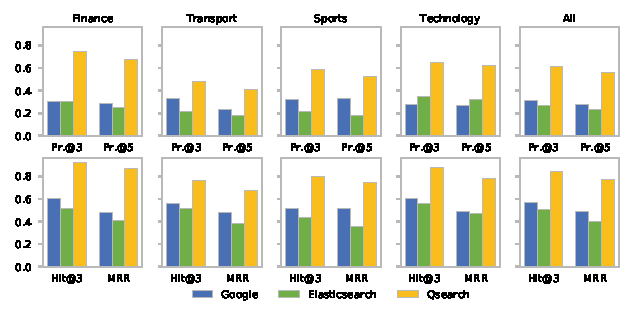
\includegraphics[width= 1\textwidth]{figures/compare.pdf}
	\caption{Comparison of Qsearch against baselines.}
	\label{fig:top-3_comparison}
\end{figure}

Overall, Qsearch performs amazingly well, typically with MRR around 0.7 or better.
The best results are for the 
Finance domain, which has the highest share in the corpus and is most represented in the
Qfact extraction training.
%Finance is the dominating slice of news articles and it covers two most frequent sample categories, Money and %Percentage, in our training dataset. 
%We can also observe that \textit{Precision@k} decreases sharply as \textit{k} increases, together with a high %\textit{MRR} and \textit{Hit} values for our both ranking models, which confirms that relevant entities are ranked higher %by our system than the irrelevant ones. 
\textit{Precision@1} is pretty good, but precision drops substantially when going deeper in the rankings. 
The embedding-based ranking model clearly outperformed the KL-divergence method
by a significant margin.
 
Figure~\ref{fig:top-3_comparison} presents the comparison of Qsearch with the $ced$ ranking model 
against Elasticsearch and Google, showing the metrics \textit{Prec.@3}, \textit{Prec.@5}, \textit{Hit@3} and \textit{MRR}. The results 
clearly indicate that Qsearch outperforms both baselines by a large margin.













%!TEX root = ../main.tex

\section{Related Work}
\label{sec:related-work}

%%%GW: keep this concise
%%% if we discuss QA at length, it suggests that these prior works are highly relevant and we should have compared to them

\subsubsection{Question Answering.} 
%Many advanced factoid-based Question Answering (QA) systems have been developed, covering the both major paradigms in QA, IR-based QA on text corpora \cite{DBLP:conf/acl/WangN15, DBLP:conf/emnlp/YangYM15} and knowledge-based QA\cite{ DBLP:conf/coling/BaoDYZZ16, DBLP:conf/ecctd/Sanchez-Azqueta17}, or fusing them both \cite{DBLP:conf/acl/DasZRM17,DBLP:conf/emnlp/SunDZMSC18}, in order to handle complex compositional queries in natural language. Diverging from traditional open-domain QA, many recently developed QA systems\cite{DBLP:journals/corr/WestonBCM15,DBLP:conf/acl/RajpurkarJL18} address the reading comprehension task that requires understanding and reasoning of natural language.  However, none of these QA systems can efficiently handle processing and reasoning of quantitative information. A few state-of-the-art works\cite{DBLP:conf/cikm/JiaARSW18} focus explicitly the reasoning of temporal constraints in questions, and most of the previous works can support mainly the counting-based numeric queries. In this work, we aim to generalize the processing of quantitative information over varied numerical constraints exploiting deep semantic role labeling. Limited number of numeric relations in the Knowledge is an important bottle neck for processing quantities, and recently has been addressed in\cite{DBLP:conf/aaai/MadaanMMRS16}. Unlike our quantity-specific context extraction model, the authors presented NumberTron which aims to extract triplets for specific numeric relations from textual corpora. Tapping into semi-structured resources from Web, QEWT\cite{DBLP:conf/kdd/SarawagiC14} harnesses ambiguous and imprecise numbers in web tables and improve the performance of quantity-seeking queries.   
%KP: discussion about WikiTableQuestions ?
QA over knowledge graphs and other linked data sources has received great attention over the
last years; see \cite{DBLP:conf/rweb/UngerFC14,DBLP:journals/kais/DiefenbachLSM18} for surveys.
State-of-the-art methods 
(e.g., \cite{DBLP:conf/acl/YihCHG15,DBLP:conf/cikm/BastH15,DBLP:conf/acl/XuRFHZ16,DBLP:conf/www/AbujabalRYW18,DBLP:journals/pvldb/ZhengYZC18}) 
translate questions into
SPARQL queries, bridging the gap between
question vocabulary and the terminology
of the underlying data by means of
templates and/or learning from
training collections of question-answer pairs.
Benchmarks like the long-standing 
QALD series and other competitions
have shown great advances along these lines
\cite{DBLP:journals/semweb/UsbeckRHCHNDU19}.
However, these benchmark tasks hardly
contain any quantity queries of the kind
addressed here (even in QALD-6-task-3, only 6 out of 150 questions are of this kind, others are mostly about quantity lookup). Note that look-ups of 
quantity attributes of qualifying entities
(e.g., Jeff Bezos's net worth, 10 richest people, or fastest sprinter over 100m)
are of a different nature, as they do not
contain quantity comparisons between query
and data (e.g., worth more than 50 million USD,
running faster than 9.9 seconds).
Moreover, the scope and diversity of the benchmark queries is necessarily restricted to relatively
few numeric properties, as knowledge graphs
hardly capture quantities in their full extent (with value and unit properly
separated and normalized). This is our motivation to tap
into text sources with more extensive coverage.

QA over text has considered a wide range
of question types (e.g., \cite{DBLP:conf/emnlp/Yang0ZBCSM18,DBLP:conf/acl/GardnerC18,DBLP:conf/acl/ChenFWB17}), but there
is again hardly any awareness of quantity queries.
Keyword search, including
telegraphic queries, with quantity conditions
have been considered by 
\cite{DBLP:conf/emnlp/JoshiSC14}, and have been applied
to web tables \cite{DBLP:journals/pvldb/PimplikarS12,DBLP:conf/kdd/SarawagiC14}. 
%The approaches pursued in that context
%cannot be carried over to our setting
%where the data input is arbitrary natural language text.

\cite{DBLP:conf/sigir/BanerjeeCR09} and
its follow-up work \cite{DBLP:conf/kdd/SarawagiC14}
focused on
a specific kind of quantity query, namely,
retrieving and aggregating numerical values
associated with an attribute of a given entity
(e.g., Bezos's net worth or GDP of India). To this end, 
learning-to-rank techniques over value distributions
were developed to
counter the uncertainty in the retrieved values,
where web pages often contain crude estimates
and lack exact values.
In contrast to our setting, that work did not
consider quantities in search conditions. 
%and did not
%require inferring units and entities to which
%quantities refer.



\subsubsection{Information Extraction.}
Recognizing and extracting numeric expressions
from text has been addressed using
techniques like CRFs and LSTMs 
(e.g., \cite{DBLP:conf/aaai/MadaanMMRS16,DBLP:conf/acl/SahaPM17,DBLP:conf/sigir/AlonsoS18}).
However, this alone does not turn numbers
into interpretable quantities, with units
and proper reference to the entity with
that quantity. Only few works attempted
to canonicalize quantities by mappings
to hand-crafted knowledge bases 
of measures \cite{DBLP:conf/cikm/IbrahimRW16}, but these efforts are
very limited in scope.
The special case of temporal expressions
has received substantial attention
(e.g., \cite{DBLP:series/synthesis/2016Strotgen}), but this solely covers dates
as measures.

Most related to our approach are the works
of \cite{DBLP:conf/kdd/SarawagiC14} and \cite{DBLP:journals/tacl/RoyVR15}.
The former used probabilistic context-free grammars
to infer units of quantities, but focused specifically
on web tables as inputs.
The latter extended semantic role labeling (see below)
to extract quantities and their units from
natural language sentences.
Neither of these can be readily applied
to extracting quantities and their reference entities
from arbitrary textual inputs.
\subsubsection{Semantic Role Labeling.} Semantic role labeling (SRL) has been intensively researched
as a building block for many 
NLP tasks \cite{DBLP:journals/coling/GildeaJ02}.
%Question Answering frameworks \cite{DBLP:conf/emnlp/ShenL07, DBLP:journals/coling/SurdeanuCZ11}, as well as, in other NLP tasks, such as Information Extraction \cite{DBLP:conf/kcap/ChristensenMSE11, DBLP:conf/naacl/StanovskyMZD18}, Machine translations \cite{DBLP:conf/coling/LiuG10}, in order to exploit the semantic representation of the predicate-argument structure of a sentence in a language. 
Given a verb phrase of a sentence
viewed as a central predicate, 
%the SRL task is to assign different pre-defined roles of the verb in the sentence. 
SRL identifies phrases that are assigned to
pre-defined roles to form a frame-like
predicate-arguments structure.
%Generally, SRL \cite{DBLP:journals/coling/GildeaJ02, DBLP:conf/conll/KoomenPRY05} is considered as a classification task based on syntactic features of sentences and often uses labeled corpus, such as PropBank \cite{DBLP:journals/coling/PalmerKG05}, FrameNet \cite{DBLP:journals/lre/Baker12}. 
%
%Instead of relying on fine-tuned syntactic features of sentences, many recent literature consider word embeddings as one of the key features to learn SRL model using different  neural network methods \cite{DBLP:conf/acl/ZhouX15, DBLP:conf/acl/HeLLZ17a, DBLP:conf/emnlp/FitzGeraldTG015}. 
Modern SRL methods make use of pre-computed
word embeddings and employ deep neural networks
for role filling (e.g., \cite{DBLP:conf/acl/ZhouX15, DBLP:conf/acl/HeLLZ17a, DBLP:conf/emnlp/FitzGeraldTG015}).
%
%Task1 of this work addresses conceptually similar to the SRL task. However, we map a sentence to a general semantic representation based on different quantity-specific roles for a given numeric value from the sentence. Hence, the characteristics of these roles differ from the predicate-argument roles where verbs are technically considered as predicates. In order to learn our quantity-specific SRL model, we employ word-embedding based deep SRL model \cite{DBLP:conf/acl/HeLLZ17a}.
Our approach differs from this state-of-the-art SRL,
as we are not primarily focused on the verb-phrase
predicate, but consider the numeric quantity in a sentence
as the pivot and aim to capture quantity-specific roles.

%%%GW: need to trim the following
To support exploration of quantitative facts in financial reports, \cite{Lamm2018QSRLA} proposed a 
semantic representation for quantity-specific roles.
% and discuss possibilities to utilize the shallow semantic parsing to develop their proposed framework. 
%In the similar direction, in order to solve the elementary school math problems, 
\cite{DBLP:journals/tacl/RoyVR15} devised a quantity representation as an additional component of
an SRL method, which is part of the Illinois Curator software suite.
% to reason about numbers in natural language. 
%
%Our SRL model represents a simplified version of their proposed semantic roles. For example, the roles \textit{entity}, \textit{value}, \textit{unit}, and \textit{resolution} are respectively similar to the roles  \textit{THEME}, \textit{VALUE with SIGN}, \textit{UNIT}, and \textit{MANNER} in their model. However, the  \textit{context} in our model generalizes the roles  \textit{QUANTITY}, \textit{LOCATION}, and \textit{TIME} together from QSRL model by Lamm et al. \cite{Lamm2018QSRLA}. Such generalization of semantic role makes our model simpler and helps in leveraging the problem of numerical Question Answering, addressed in this work. 
Our approach makes use of this technique,
%which is part of the Illinois Curator software suite,
as a preprocessing step.
However, we go further by 
learning how to connect quantities with their
respective entities and to collect relevant 
context cues that enable our matching and
ranking stage for query answering.




%!TEX root = ../main.tex

\section{Conclusion}
%We presented a method for learning rules that may contain negated atoms from KGs that
%dynamically exploits feedback from a precomputed embedding model. 
%Our approach is general in that any embedding model can be utilized including text-enhanced ones, which indirectly allows us to 
%harness
%unstructured 
%web sources 
%for rule learning.
% We evaluated our approach with various configurations on real-world datasets and observed significant improvements
%over state-of-the-art rule learning systems.\looseness=-1
%
%An interesting future direction is to extend our work to more complex non-monotonic rules with higher-arity predicates,
%aggregates and existential variables or disjunctions in rule heads, which is challenging due to inevitable scalability issues.

Awareness of entities and types has greatly advanced semantic search
both for querying the web of linked data and for Internet search engines.
In contrast, coping with quantities in text content and in query constraints
has hardly received any attention, yet is an important case.
This paper has presented the Qsearch system for full-fledged support of
quantity queries, through new ways of information extraction and 
answer matching and ranking.
We capture quantities in their full extent, including units of measures,
reference entities and the relevant contexts.
The model for Qfacts and Qqueries is relatively simple but highly versatile and effective.
%a more detailed structured modeling would not be able to cope with the
%uncertainty in textual inputs and the approximate matching of candidate answers.
A key asset of Qsearch is its high quality in extracting Qfacts,
recognizing the right entity-quantity pairs even in complex sentences.

Future work includes devising additional ways of aggregating Qfacts with
the same candidate answer, so as to obtain strong signals from many
noisy cues (i.e., when the same entity-quantity pair occurs in many pages,
but mostly in the form of crude estimates or vague hints).
Also, we plan to extend the Qquery model to incorporate queries that
contain multiple quantity conditions (e.g., hybrid SUVs with range above 500 miles
and energy consumption above 40 MPGe).








%\paragraph*{Acknowledgements.}

%\documentclass[a4paper]{llncs}

%\documentclass{llncs}
%
\usepackage[T1]{fontenc}
\usepackage{lmodern}
\usepackage[utf8]{inputenc}
\usepackage{amsfonts}
\usepackage{eurosym}
\usepackage{amsmath}
\usepackage{amssymb}
\usepackage{booktabs}
\usepackage{makeidx}  % allows for indexgeneration
\usepackage{epsfig} 
\usepackage{cite}
\usepackage{color}
\usepackage{multirow}
\usepackage{mathtools}
\usepackage{subfig}
\usepackage{hyperref}
\usepackage[para]{footmisc}
\hypersetup{
    colorlinks=true,
    %linkcolor=blue,
%    filecolor=magenta,      
    urlcolor=blue,
    citecolor=blue,
    linkcolor=blue,
}

\usepackage[inline]{enumitem}


\usepackage{llncs-space}

\newcommand{\G}{\ensuremath{\mathcal{G}}\xspace}
\newcommand{\X}{\ensuremath{\mathcal{X}}\xspace}
\newcommand{\C}{\ensuremath{\mathcal{C}}\xspace}
\newcommand{\R}{\ensuremath{\mathcal{R}}\xspace}
\newcommand{\PG}{\ensuremath{\mathcal{P}}\xspace}
\newcommand{\PW}{\ensuremath{\mathsf{PW}}\xspace}
\newcommand{\sem}[1]{[|#1|]}
\newcommand{\set}[1]{\{#1\}}
\newcommand{\incl}{\subseteq}
\renewcommand{\L}{\ensuremath{\mathcal{L}}\xspace}

\newtheorem{task}{Task}


%%% \squishlist definition, list with reduced margins
\newcommand{\squishlist}{
 \begin{list}{$\bullet$}
  { \setlength{\itemsep}{0pt}
     \setlength{\parsep}{3pt}
     \setlength{\topsep}{3pt}
     \setlength{\partopsep}{0pt}


     \setlength{\leftmargin}{1em}
     \setlength{\labelwidth}{1em}
     \setlength{\labelsep}{0.5em} } }

\newcommand{\squishlisttwo}{
 \begin{list}{$\bullet$}
  { \setlength{\itemsep}{0pt}
    \setlength{\parsep}{0pt}
    \setlength{	opsep}{0pt}
    \setlength{\partopsep}{0pt}
    \setlength{\leftmargin}{2em}
    \setlength{\labelwidth}{1.5em}
    \setlength{\labelsep}{0.5em} } }

\newcommand{\squishend}{
  \end{list}  }
%\renewcommand{\baselinestretch}{0.99}

\begin{document}
%
\frontmatter          
%



\pagestyle{headings}  

\mainmatter               
%
\title{Qsearch: Answering Quantity Queries from Text}

\author{%
Vinh Thinh Ho$^{1}$,\ \ 
Yusra Ibrahim$^{1}$,\ \ 
Koninika Pal$^{1}$,\\
Klaus Berberich$^{1,2}$,\ \ 
and Gerhard Weikum$^{1}$
}		
\institute{
$^1\ $Max Planck Institute for Informatics, Saarbr\"ucken, Germany\\
$^2\ $Saarland University of Applied Sciences, Saarbr\"ucken, Germany
}


\maketitle        

\begin{abstract}
%%%Motivation and Problem
Quantities appear in search queries in numerous forms: 
%to find a products within a specific price range, 
%to locate a country with an increasing GDP, to identify athletes who won multiple Olympic medals, among others.
companies with annual revenue of at least 50 Mio USD,
athletes who ran 200 meters faster than 19.5 s, 
electric cars with range above 400 miles, and so on.
Processing such queries requires the understanding of numbers present in the query to capture the contextual information about the queried entities. 
Modern search engines and QA systems
%like Google, Bing, etc. 
can 
%efficiently 
handle queries
that involve entities and types, 
%which need to exploit only relational structures embedded in Web content and social media for queried entities. 
%But they fail to produce crisp answers to the queries involving numerical constraints as they disregard the reasoning %over quantitative information.
but they often fail on properly interpreting quantities in queries and candidate answers
when the specifics of the search condition (less than, above, etc.), the units of interest (seconds, miles, meters, etc.)
and the context of the quantity matter (annual or quarterly revenue, etc.).
%  
%Numeric answers for such queries might appear in various sources, either structured (e.g. tables, lists), or unstructured (e.g. text), where processing unstructured text are more challenging. 
%Modern search engines like Google, Bing, etc. support queries that involve relational structures embedded in Web content and social media and can provide crisp answers to the queries or questions. However, informative quantities are usually disregarded. 
%
%Approach and  Contribution
In this paper, we present a search and QA system, called Qsearch, 
that  
%tackles queries with numerical constraints by harnessing quantitative  contextual information about entities from text.
can effectively answer advanced queries with quantity conditions.
%In particular, we propose a framework for representing quantitative information, 
Our solution is based on a deep neural network for extracting quantity-centric tuples from text sources,
%an efficient deep neural network for extracting these information from textual data, 
and a novel matching model to 
%produce 
retrieve and rank
answers 
%for given numerical queries. 
from news articles and other web pages.
Experiments 
%on real-world data 
demonstrate the effectiveness of Qsearch on benchmark queries collected by crowdsourcing.

\end{abstract}

\begin{keywords}
Semantic Search, Question Answering, Information Extraction, 
%Numeric 
Quantities
\end{keywords}

\input{sections/10-intro}
\input{sections/20-CompModelSysOverview}
\input{sections/30-numerical_fact_extraction.tex}
\input{sections/40-matching.tex}
\input{sections/60-evaluation.tex}
\input{sections/70-related_work.tex}
\input{sections/80-conclusion.tex}



%\paragraph*{Acknowledgements.}

%\input{main.bbl}

\bibliographystyle{abbrv}
\bibliography{references}


\end{document}


\bibliographystyle{abbrv}
\bibliography{references}


\end{document}


\bibliographystyle{abbrv}
\bibliography{references}


\end{document}


\bibliographystyle{abbrv}
\bibliography{references}


\end{document}
